% ==========================================================================
% Devorix --- Investor PRD
% Modular report-class document. Compile with: xelatex, bibtex, xelatex, xelatex
% ==========================================================================
\documentclass[11pt,a4paper,oneside]{report}

% ---- Fonts (xelatex / unicode, needed for the rupee sign U+20B9) ----------
\usepackage{fontspec}
\setmainfont{DejaVu Serif}
\setsansfont{DejaVu Sans}
\setmonofont{DejaVu Sans Mono}

% ---- Page geometry & headers ----------------------------------------------
\usepackage[a4paper,margin=1in]{geometry}
\usepackage{fancyhdr}
\pagestyle{fancy}
\fancyhf{}
\renewcommand{\headrulewidth}{0.4pt}
\fancyhead[L]{\small\textit{Devorix --- Investor PRD}}
\fancyhead[R]{\small\textit{\leftmark}}
\fancyfoot[C]{\thepage}
\renewcommand{\chaptermark}[1]{\markboth{#1}{}}

% ---- Core packages ---------------------------------------------------------
\usepackage{graphicx}
\usepackage{booktabs}
\usepackage{longtable}
\usepackage{array}
\usepackage[table]{xcolor}
\usepackage{tcolorbox}
\tcbuselibrary{breakable,skins}
\usepackage{enumitem}
\usepackage{hyperref}
\hypersetup{
  colorlinks=true,
  linkcolor=blue!50!black,
  citecolor=green!40!black,
  urlcolor=blue!60!black,
  bookmarksopen=true,
  pdftitle={Devorix --- Investor PRD},
  pdfauthor={Devorix}
}
\usepackage[round]{natbib}
\usepackage{titlesec}
\usepackage{titling}
\usepackage{caption}
\captionsetup{font=small,labelfont=bf}

% ---- TikZ / pgfplots --------------------------------------------------------
\usepackage{tikz}
\usetikzlibrary{positioning,arrows.meta,shapes.geometric,calc,shadows,decorations.pathreplacing}
\usepackage{pgfplots}
\pgfplotsset{compat=1.18}

% ---- Misc convenience -------------------------------------------------------
\setlength{\parskip}{0.5em}
\setlength{\parindent}{0pt}
\renewcommand{\arraystretch}{1.15}

% ---- Rupee symbol (some chapters use \textrupee instead of the literal ₹ glyph) ----
\providecommand{\textrupee}{₹}

% ---- Confidence-label macros (Verified fact / Industry estimate / Internal assumption) ----
\newcommand{\verifiedfact}{\textcolor{green!35!black}{\textbf{[Verified fact]}}}
\newcommand{\industryestimate}{\textcolor{orange!70!black}{\textbf{[Industry estimate]}}}
\newcommand{\internalassumption}{\textcolor{red!50!black}{\textbf{[Internal assumption]}}}

\title{\Huge\textbf{Devorix}\\[0.3em]\Large Investor-Grade Product \& Strategy PRD}
\author{Devorix}
\date{June 2026}

\begin{document}

% ---------------------------------------------------------------------------
\begin{titlepage}
  \centering
  \vspace*{2cm}
  {\Huge\bfseries Devorix\par}
  \vspace{0.5cm}
  {\Large Investor-Grade Product, Market \& Strategy PRD\par}
  \vspace{1.5cm}
  {\large\itshape Wait-state advertising for AI coding agents --- an India-native, developer-revenue-shared alternative to Kickbacks.ai\par}
  \vspace{2cm}
  {\large June 2026\par}
  \vspace{1cm}
  {\normalsize\itshape Pre-seed stage. Honest seed-stage framing throughout: every claim is labeled\\
  \verifiedfact\ \industryestimate\ or \internalassumption.\par}
  \vfill
  {\small Prepared as an internal strategy document. Not a solicitation of investment.\par}
\end{titlepage}

\tableofcontents
\listoffigures
\listoftables
\clearpage

% ---------------------------------------------------------------------------
% Chapters
% ---------------------------------------------------------------------------
\chapter{Executive Summary}
\label{ch:executive-summary}

\section{The idea, in one line}

When an AI coding tool is ``thinking,'' it shows a status line that earns
nothing. Devorix puts a small, tasteful sponsor line there and shares the money
with the developer --- paid in rupees over UPI. India first; global is an
explicit Phase~2.

\section{The honest current stage}

This document is written from pre-seed reality, not seed-stage aspiration, and
the framing here governs every chapter that follows. Devorix is
\textbf{pre-launch and pre-revenue}: zero advertisers signed, zero installs, a
\textbf{solo founder} building the MVP, and a total budget of approximately
\textbf{₹1~lakh} on a deliberately low-burn, sweat-equity basis (founder
salary modelled at ₹0). The category itself is roughly 2.5~weeks old (born
2026-06-11), and \emph{nobody in it is making real money yet} --- not even the
leaders Kickbacks and IdleAds, both of which used Firecrawl as an
\emph{unpaid} house placeholder rather than a paying customer
\citep{masterplan_2026}.

This is therefore a pre-seed / accelerator-stage story. The honest ask is
``give us a small check or an accelerator slot to prove the loop works,'' not
``fund a billion-dollar vision.'' We keep those two registers strictly
separate throughout, because mixing infrastructure-scale ambition with a
fund-a-14-day-sprint ask is the single most common way pre-seed pitches lose
credibility with experienced investors.

\section{The locked business model}

The following decisions are final and are not reopened anywhere in this
document (the complete locked-decisions table appears in
Appendix~\ref{app:locked-decisions}):

\begin{itemize}
  \item \textbf{Revenue share = 50/50} between Devorix and the developer.
  \item \textbf{Hybrid pricing ladder.} Tier~0 (house ads + flat monthly
        sponsorships of ₹10{,}000--15{,}000/mo, until $\sim$5
        advertisers) $\rightarrow$ Tier~1 (fixed-price CPM rate card, once
        5--10 advertisers signed) $\rightarrow$ Tier~2 (real-time auction,
        once 5{,}000+ DAU).
  \item \textbf{Payout threshold = ₹300}, settled automatically over UPI
        via the RazorpayX Payouts API \citep{razorpayx_2026}.
  \item \textbf{5-second billable impression} for the v1 build; 10~seconds
        kept as a documented, data-gated option.
  \item \textbf{USD$\rightarrow$INR = ₹94} used everywhere.
  \item \textbf{Client = non-patching status-bar overlay} on Claude Code ---
        never patches the renderer, never reads code or prompts, never touches
        Claude's OAuth tokens.
\end{itemize}

\section{Headline market and financial numbers}

The surrounding pools are large and favourable as \emph{context}, not as a
funnel that can be divided down to a Devorix forecast:

\begin{itemize}
  \item \textbf{India developers on GitHub: 27~million (2026)}, up from 21.9M
        in October 2025, projected to reach 57.5M by 2030 (Satya Nadella, on
        record) \citep{masterplan_2026}. \emph{(Verified fact.)}
  \item \textbf{Claude Code --- Devorix's first target tool --- went \$0 to a
        \$2.5B run-rate in 9 months}; 85--92\% of developers now use AI coding
        tools \citep{masterplan_2026}. \emph{(Verified fact.)}
  \item Adjacent anchors: the developer-tools market is \$7.4--8.8B (2026), AI
        code tools $\sim$\$9--9.5B; the closest business-model analogue,
        affiliate marketing, is $\sim$\$20B (2026). \emph{(Industry
        estimate.)}
  \item \textbf{The locked 4-month plan (audited, not modelled):} 500 installs
        and 3 advertisers by month~4, ₹45{,}000/mo revenue, and a
        cumulative net of $\sim$\textbf{₹39{,}500}. Everything past
        month~4 is gated planning scaffolding, not a funded forecast.
        \emph{(Verified locked input.)}
\end{itemize}

The single most important structural insight: the funnel from market to
captured revenue does \emph{not} narrow on the developer side --- 27M India
developers is abundant and cheap to reach. The binding constraint is
\textbf{advertiser demand}, which has no market-sizing number yet because
nobody in this young category has found it.

\section{The single biggest risk and the single biggest open question}

\textbf{Biggest risk: zero verified paying advertisers exist anywhere in this
category.} Nobody has yet proven that a developer-tool brand will pay for a
\emph{wait-state} placement at any price. This is a larger risk than any
product, platform, or compliance concern, and the 14-day sprint exists
precisely to test it: one verbal yes from a cold advertiser pitch means go,
zero means stop and rethink.

\textbf{Biggest open question: will developers retain past the novelty?}
Developers are skeptical rather than excited --- Kickbacks' own Show~HN drew
2~points and 0~comments, and the loudest reaction across the category has been
privacy suspicion, not demand. This is a monetization opportunity layered onto
an existing attention pool, not a pain point developers are asking to solve.
Only real installs plus week-4 retention data will answer whether a developer
keeps the client once the rupee sum (₹100--200/month at realistic usage)
is no longer novel.

\section{The ask}

The honest ask matches the stage: a small pre-seed check or an accelerator
slot to fund the 14-day sprint and the 4-month loop-proving plan. The gate that
should govern any decision to continue --- ours and an investor's --- is the
locked go/no-go test: at least two advertisers paid \emph{and} renewed,
week-4 developer retention holds, and the founder still wants to run it on tiny
margins. If any axis fails, the right outcome is to stop having spent
$\sim$₹20--30k and a few weekends to learn what most founders pay far more
to discover. This is not a maximalist pitch; it is a request to fund the
cheapest credible test of a real, timely, demand-side-constrained opportunity.

\section*{Vision, not the near-term ask}
\addcontentsline{toc}{section}{Vision, not the near-term ask}

\emph{The following is long-term direction, explicitly not the thing being
underwritten today.} If the near-term loop works, the same clean ledger and
payout primitives built at v1 become the foundation for a broader bet:
Devorix could grow from a wait-state sponsorship layer into India's
trust-and-payout rail for developer-attention monetization, and eventually
into financial infrastructure for the emerging agent economy --- a space where
Visa, Mastercard, PayPal, Stripe, and Google all shipped agentic-payment
infrastructure within a single six-month window. The defensible reason to
build clean attribution and ledger discipline \emph{now} is that it makes that
optionality real later at almost no extra cost today. But the vision is the
reason the infrastructure bet is worth taking \emph{if} the loop proves out
--- it is not the bet itself, and it is not what we are asking anyone to fund
at this stage.

\chapter{The Problem}
\label{ch:problem}

\section{Dead inventory in the thinking status line}

Every time an AI coding agent pauses to ``think,'' it renders a status line ---
a spinner, a shimmer, a few words of ephemeral text --- that conveys nothing of
commercial value and earns nothing for anyone. With 85--92\% of developers now
using AI coding tools and the most engaged among them spending 4--10 hours a
day inside them, this adds up to an enormous, continuously refreshed pool of
captive, full-attention wait-state moments \citep{masterplan_2026}. The
moment is unusually valuable as an attention surface precisely because it is
\emph{not} a sidebar a user scrolls past: the developer is waiting, watching,
and briefly idle. Today that attention is simply discarded. It is dead
inventory.

The scale of the underlying surface is not speculative. Claude Code ---
Devorix's first target tool --- grew from \$0 to a \$2.5B run-rate in nine
months, and Cursor reached $\sim$\$2B annualized revenue with over a million
paying customers \citep{masterplan_2026}. \emph{(Verified fact.)} Real,
large, fast-growing engagement is flowing through the exact surface where this
wait-state moment occurs.

\section{Developers earn nothing from the time they spend}

Developers spend that wait time --- and the broader hours they pour into AI
coding tools --- without any financial participation in the value their
attention represents. For the large under-monetized developer base this is a
structural mismatch: GitHub Sponsors supported 49{,}148 developers as of March
2026, yet 60\% of surveyed open-source maintainers describe themselves as
unpaid hobbyists and only 13\% as professional or paid
\citep{customerproduct_2026}. \emph{(Verified fact.)} A large population is
structurally primed to want incremental income attached to tools they already
use.

We are deliberately honest about the shape of this problem, following the
plan's own VC-lens validation \citep{masterplan_2026}. This is
\textbf{a monetization opportunity layered onto an existing attention pool, not
a pain point developers are actively trying to solve}. Developers are not
asking for this. The closest behavioural precedent --- cashback browser
extensions that retain users because the reward appears ambiently inside an
existing workflow rather than requiring a separate action --- is encouraging
for adoption but is consumer shopping, not developer tooling
\citep{customerproduct_2026}. \emph{(Industry estimate.)} The pain that is
genuinely severe sits on the \textbf{advertiser} side: developer-tool marketers
have shockingly few high-trust placement options built for the agentic-coding
moment, with Carbon Ads (audited at \$1.60 CPM, selling to Okta, GitLab and
MongoDB) essentially the only mature one, and it was never built for this
moment specifically \citep{masterplan_2026}.

\section{A working competitor exists --- but structurally cannot pay India}

The wait-state advertising mechanic is not hypothetical. Kickbacks.ai launched
on 2026-06-11 and its launch tweet passed 5.5~million views in 24~hours; a
direct clone, IdleAds.dev, appeared within 24~hours of it
\citep{masterplan_2026}. \emph{(Verified fact.)} The category has real
top-of-funnel virality. But it has a structural hole that defines Devorix's
wedge:

\textbf{Kickbacks --- and the Stripe-based model generally --- structurally
cannot pay out to India.} As of June~2026, Kickbacks had not yet activated real
payouts; its Stripe Connect integration was reported ``nearing completion''
\citep{masterplan_2026}. The reason is independently re-verified beyond a
single GitHub issue, against Stripe's own support documentation: Stripe has
been invite-only for new India accounts since May~2024 due to RBI regulatory
changes, and Connect Express onboarding for India-based recipients is
restricted \citep{stripe_india_2026}. Confidence on this wedge is
\textbf{High}. The same Stripe-India gap that is slowing the category leader is
exactly what Devorix is built around: native, automated, GST-ready UPI payouts
via RazorpayX, which supports automated UPI/IMPS/NEFT/RTGS with 24/7 instant
settlement \citep{razorpayx_2026}.

We are careful not to overclaim here. IdleAds.dev already does UPI
\emph{manually}, so the payout-rail edge is \emph{contested, not exclusive} ---
the real differentiator is native, automated, GST-ready UPI done properly,
not merely ``we pay India'' \citep{masterplan_2026}.

\section{Why this is a real, timely problem}

The timing is right, narrowly, on three converging facts
\citep{masterplan_2026}:

\begin{enumerate}
  \item \textbf{Adoption just crossed the majority case.} AI coding tools moved
        from early-adopter to mainstream (85--92\% of developers), so the
        attention pool the mechanic monetizes is now genuinely large.
        \emph{(Verified fact.)}
  \item \textbf{India is the fastest-growing developer base anywhere} --- 27M
        on GitHub in 2026, projected 57.5M by 2030, with India among the
        highest-adoption regions for AI coding tools --- yet it is the one
        large market the dominant Stripe-based payout model cannot serve.
        \emph{(Verified fact / India-specific adoption: Industry estimate.)}
  \item \textbf{The bottleneck is wide open.} Zero verified paying advertisers
        exist anywhere in this category; the real constraint is demand-side
        sales, which every competitor is failing at while racing the same
        shallow mechanic \citep{masterplan_2026}. \emph{(High confidence ---
        absence of evidence corroborated across a 3-day pulse-check.)}
\end{enumerate}

The honest read from the plan's VC-lens validation is preserved here without
softening: the window is short and the moat is shallow --- IdleAds cloned
Kickbacks' mechanic within 24~hours --- so timing favours moving fast on the
demand side, where the real, severe, currently-unmet need lives, rather than on
product polish on the supply side, where developers are mildly interested at
best \citep{masterplan_2026}. The problem Devorix addresses is therefore
real and timely, but its sharpest edge is the advertiser's missing high-trust
India-payable placement, not a developer crying out to be paid.

\chapter{Market Research: TAM, SAM, and SOM}
\label{ch:market-research}

\section*{How to read this chapter}

This chapter carries two registers that must not be blurred together. The first is the near-term reality and the ask: Devorix is pre-launch, pre-revenue, with zero advertisers signed, zero installs, a solo founder, and a \textrm{\textrupee}1 lakh total budget. The numbers that matter for the funding conversation today are the locked four-month plan and the go/no-go gate it feeds (MASTER-PLAN \S 8.3). This is a pre-seed / accelerator-stage story --- ``give us a small check or a slot to prove the loop works'' --- not a seed-round forecast.

The second register is the long-term vision, clearly labeled as vision. The TAM ceiling math and the agentic-economy market context are \emph{optionality and direction}, not the thing being underwritten. They answer ``why is this infrastructure bet worth taking if the near-term loop works,'' not ``fund our billion-dollar projection.''

Every figure in this chapter carries one of three labels, used consistently and never blurred through synthesis:

\begin{itemize}
  \item \textit{[Verified fact]} --- named, on-record, or independently multi-sourced.
  \item \textit{[Industry estimate]} --- published by research firms or third parties, directionally consistent but without a single authoritative number.
  \item \textit{[Internal assumption]} --- Devorix's own model output or extrapolation; not a researched fact.
\end{itemize}

No locked decision (50/50 revenue split, \textrm{\textrupee}300 payout threshold, hybrid pricing ladder, 5-second impression, \textrm{\textrupee}94 FX, India-first / Global-Phase-2) is reopened here. All locked numbers are carried forward as given.

\section{A reconciliation note on adoption-share figures}
\label{sec:adoption-reconciliation}

Two of our inputs carry different numbers for Claude Code / Cursor adoption, and rather than silently dropping either, we resolve the discrepancy explicitly here.

MASTER-PLAN \S 10 states that ``Cursor and Claude Code are tied at 18\% workplace usage each'' \textit{[Verified fact --- high confidence, converging independent surveys]} \cite{masterplan_2026}. A more recent 2026 survey aggregation, by contrast, reports that among agentic-tool users specifically, the primary-tool split is Claude Code 28\% / Cursor 24\% \textit{[Industry estimate --- single aggregation source]} \cite{agentictoolsurvey_2026}.

\textbf{These are not contradictory --- they measure different things.} The 18\%/18\% figure is workplace usage of any kind across the whole developer population; the 28\%/24\% figure is primary-tool selection among the subset who already use agentic tools regularly. A higher number on a narrower, more-engaged base is exactly what one would expect.

\textbf{Decision for this PRD:} we use 18\% workplace usage (MASTER-PLAN \S 10) as the headline adoption anchor, because it is the better-sourced, more conservative figure, and because it matches the convention used everywhere else in the plan. We carry the 28\%/24\% primary-tool split forward as a directional, favorable signal for Claude Code's momentum (consistent with the ``\$0 \(\to\) \$2.5B Claude Code run-rate in 9 months'' data point) --- \emph{not} as a planning number.

\textbf{Flag for the next funding conversation:} the 28\%/24\% figure should be re-verified against a second independent source before being quoted to an investor. It currently rests on a single 2026 aggregation. It is recorded here, not dropped.

\section{Top-down: adjacent market anchors}
\label{sec:top-down}

None of the markets below measure Devorix's niche --- wait-state sponsorship on AI coding tools --- directly. They establish that the surrounding dollar pools are large and real. They cannot be divided down to produce a credible Devorix TAM; that is a genuine gap, flagged in Section~\ref{sec:open-questions-market}.

\begin{table}[htbp]
\centering
\caption{Adjacent market anchors (top-down, scale context only)}
\label{tab:adjacent-markets}
\small
\begin{tabular}{p{4.0cm}p{5.3cm}p{3.0cm}}
\toprule
\textbf{Market} & \textbf{Size} & \textbf{Label} \\
\midrule
AI code tools market (narrow def.) & \$9.35B (2026); \$7.65B (2025) \(\to\) \$9.46B (2026) across firms & \textit{Industry estimate} \cite{aicodetools_2026} \\
AI code tools market (broad def., incl. review/testing/platforms) & \$29.47B (2025) \(\to\) \$34.58B (2026) & \textit{Industry estimate} (wide range reflects category-boundary disagreement) \cite{aicodetoolsbroad_2026} \\
Enterprise AI coding agents (Gartner) & \textasciitilde\$9.8--11.0B annualized (Apr 2026) & \textit{Verified fact} \cite{gartner_2026} \\
Claude Code run-rate (Devorix's first target tool) & \$0 \(\to\) \$2.5B run-rate in 9 months & \textit{Verified fact} (total tool revenue, \emph{not} an ad-monetization figure) \cite{anthropic_2026} \\
Cursor (Anysphere) & \textasciitilde\$2B annualized rev., 1M+ paying customers, \$29.3B valuation (Nov 2025) & \textit{Verified fact} (named funding sources) \cite{anysphere_2025} \\
Developer tools market, global & \$7.44--8.8B (2026) \(\to\) \$15.72B by 2031 (\textasciitilde16\% CAGR) & \textit{Industry estimate} --- closest ``category'' anchor to Devorix's surface \cite{devtoolsmarket_2026} \\
Affiliate marketing, global (closest business-model analogue) & \$20.07B (2026) \(\to\) \$82.64B (2035) at 15.2\% CAGR; alt.\ \textasciitilde\$23.84B (2026) platform-layer only & \textit{Industry estimate} --- no developer-focused sub-segment isolated by any source \cite{affiliatemarketing_2026} \\
Agentic commerce / agent economy by 2030 & \$3--5T (McKinsey); narrower cuts \$190--500B (Morgan Stanley / Bain, US only) & \textit{Industry estimate} --- long-range, \textbf{not} a near-term TAM \cite{mckinsey_2026} \\
Dev-ad-platform benchmarks & daily.dev \$5,000--15,000/mo minimum spend, CPM \$10--20; SaaS spend \textasciitilde8\% of ARR on marketing & \textit{Industry estimate} --- sanity check: Devorix Tier-0 \textrm{\textrupee}10--15k/mo (\textasciitilde\$120--180) is far below the cheapest mainstream dev-ad minimum \cite{dailydev_2026} \\
\bottomrule
\end{tabular}
\end{table}

\textbf{Top-down read:} the correct top-down framing is narrow. Devorix competes for a slice of the dev-marketing budgets that already exist (\$5k--15k+/mo per advertiser on Carbon Ads, daily.dev, and dev newsletters today). The developer-tools market (\$7.4--8.8B, 2026) and the dev-marketing-spend layer on top of it are the right-order-of-magnitude pools Devorix's advertiser revenue is drawn from --- \textbf{not} the multi-trillion agentic-commerce figures, which are vision-context only.

\begin{figure}[htbp]
\centering
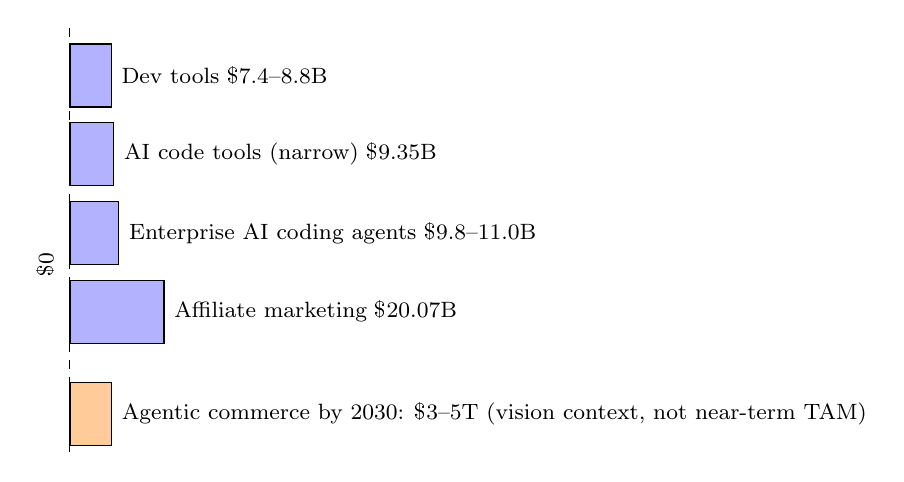
\begin{tikzpicture}[
  every node/.style={font=\small},
  bar/.style={draw, fill=blue!30, minimum height=0.8cm},
  visionbar/.style={draw, fill=orange!40, minimum height=0.8cm}
]
\def\scale{0.0017}
\node[bar, minimum width=8.8*\scale*1000, anchor=west] (b1) at (0,0) {};
\node[anchor=west, font=\footnotesize] at (b1.east) {Dev tools \$7.4--8.8B};

\node[bar, minimum width=9.35*\scale*1000, anchor=west] (b2) at (0,-1) {};
\node[anchor=west, font=\footnotesize] at (b2.east) {AI code tools (narrow) \$9.35B};

\node[bar, minimum width=10.4*\scale*1000, anchor=west] (b3) at (0,-2) {};
\node[anchor=west, font=\footnotesize] at (b3.east) {Enterprise AI coding agents \$9.8--11.0B};

\node[bar, minimum width=20.07*\scale*1000, anchor=west] (b4) at (0,-3) {};
\node[anchor=west, font=\footnotesize] at (b4.east) {Affiliate marketing \$20.07B};

\node[visionbar, minimum width=15, anchor=west] (b5) at (0,-4.3) {};
\node[anchor=west, font=\footnotesize] at (b5.east) {Agentic commerce by 2030: \$3--5T (vision context, not near-term TAM)};

\draw[dashed] (0,0.6) -- (0,-4.8);
\node[font=\footnotesize, rotate=90] at (-0.3,-2.4) {\$0};
\end{tikzpicture}
\caption{Adjacent-market scale comparison (top-down anchors). The agentic-commerce figure is drawn at a compressed, visually distinct scale and flagged as vision context, not a near-term TAM input.}
\label{fig:adjacent-markets}
\end{figure}

\section{Bottom-up: India developer base to realistic capture}
\label{sec:bottom-up}

\begin{table}[htbp]
\centering
\caption{Bottom-up funnel: India developer base to agentic-tool pool}
\label{tab:bottom-up-funnel}
\small
\begin{tabular}{p{4.3cm}p{5.0cm}p{3.2cm}}
\toprule
\textbf{Step} & \textbf{Figure} & \textbf{Label} \\
\midrule
India developers on GitHub, 2026 & \textbf{27 million} (up from 21.9M Oct 2025; 2M+ added in 2026) & \textit{Verified fact} (GitHub COO Kyle Daigle, multi-source) \cite{github_2026} \\
India developers on GitHub, 2030 projection & \textbf{57.5 million} (projected largest GitHub community globally) & \textit{Verified fact} (Satya Nadella, on record) \cite{nadella_2026} \\
Developers using any AI coding tool & 85--92\% global; India \textgreater 97\% have used, \textgreater 80\% regular use (among highest of any region) & Global = \textit{Verified fact} \cite{masterplan_2026}; India-specific = \textit{Industry estimate} \\
Using AI coding agents specifically (Devorix's actual surface) & Global \textasciitilde 55\% of devs regularly use AI agents; primary-tool split Claude Code 28\% / Cursor 24\% (see \S\ref{sec:adoption-reconciliation}) & \textit{Industry estimate} --- agentic use \(\neq\) autocomplete; Copilot's broad 58\% ``any-use'' is mostly autocomplete \cite{agentictoolsurvey_2026} \\
Implied India agentic-tool pool, 2026 & Working range \textbf{5--15M} (applying global \textasciitilde 55\% to 27M base; conservative cut for India's newer agentic penetration) & \textbf{\textit{Internal assumption}} --- built by applying a global ratio to the India base; no India-specific agentic-only survey exists \\
\bottomrule
\end{tabular}
\end{table}

\textbf{A deliberately conservative SAM stance:} the 5--15M range above is the outer envelope. MASTER-PLAN \S 3's more conservative ``single-digit millions'' framing is the safer planning assumption until India-specific primary research exists (an open question, Section~\ref{sec:open-questions-market}). We adopt single-digit-millions as the working SAM and treat 5--15M as the ceiling, not the plan.

\begin{figure}[htbp]
\centering
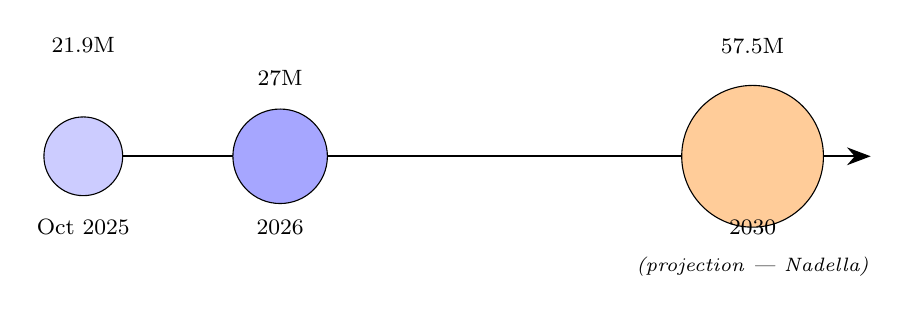
\begin{tikzpicture}[
  every node/.style={font=\small},
  dot/.style={draw, circle, fill=blue!20, minimum size=8mm},
  lbl/.style={font=\footnotesize}
]
\draw[-{Stealth[length=3mm]}, thick] (0,0) -- (10,0);
\foreach \x/\y in {0/2025.8, 2.5/2026, 8.5/2030} {
  \draw (\x,0.12) -- (\x,-0.12);
}
\node[dot, minimum size=10mm] at (0,0) {};
\node[lbl, above=2mm of {(0,0.4)}] at (0,1.0) {21.9M};
\node[lbl] at (0,-0.9) {Oct 2025};

\node[dot, minimum size=12mm, fill=blue!35] at (2.5,0) {};
\node[lbl] at (2.5,1.0) {27M};
\node[lbl] at (2.5,-0.9) {2026};

\node[dot, minimum size=18mm, fill=orange!40] at (8.5,0) {};
\node[lbl] at (8.5,1.4) {57.5M};
\node[lbl] at (8.5,-0.9) {2030};
\node[lbl, font=\scriptsize\itshape] at (8.5,-1.4) {(projection --- Nadella)};
\end{tikzpicture}
\caption{India developer population on GitHub: growth trajectory. 2030 figure is a projection, not a measured value.}
\label{fig:india-dev-growth}
\end{figure}

\section{Adoption split (cross-referenced)}
\label{sec:adoption-split}

\begin{figure}[htbp]
\centering
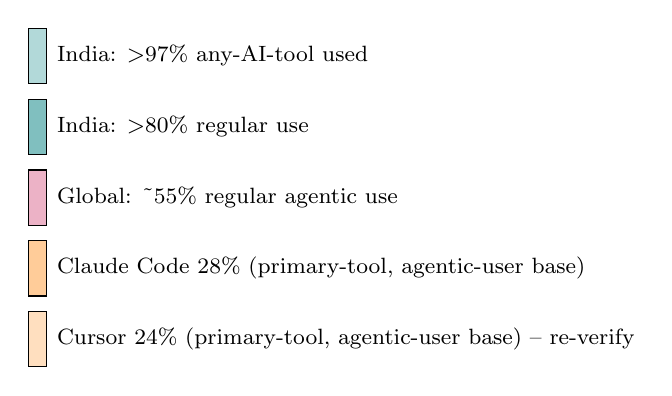
\begin{tikzpicture}[
  every node/.style={font=\small},
  hbar/.style={draw, fill=teal!30, minimum height=0.7cm},
]
\def\scl{0.06}
\node[hbar, minimum width=97*\scl, anchor=west] (r1) at (0,0) {};
\node[anchor=west, font=\footnotesize] at (r1.east) {India: \textgreater 97\% any-AI-tool used};

\node[hbar, minimum width=80*\scl, anchor=west, fill=teal!50] (r2) at (0,-0.9) {};
\node[anchor=west, font=\footnotesize] at (r2.east) {India: \textgreater 80\% regular use};

\node[hbar, minimum width=55*\scl, anchor=west, fill=purple!30] (r3) at (0,-1.8) {};
\node[anchor=west, font=\footnotesize] at (r3.east) {Global: \textasciitilde 55\% regular agentic use};

\node[hbar, minimum width=28*\scl, anchor=west, fill=orange!40] (r4) at (0,-2.7) {};
\node[anchor=west, font=\footnotesize] at (r4.east) {Claude Code 28\% (primary-tool, agentic-user base)};

\node[hbar, minimum width=24*\scl, anchor=west, fill=orange!25] (r5) at (0,-3.6) {};
\node[anchor=west, font=\footnotesize] at (r5.east) {Cursor 24\% (primary-tool, agentic-user base) -- re-verify};
\end{tikzpicture}
\caption{Adoption split across measurement bases. Rows 4--5 (primary-tool split, 28\%/24\%) are flagged for re-verification against a second source; see the note below.}
\label{fig:adoption-split}
\end{figure}
{\small\itshape Note: MASTER-PLAN \S 10 anchors workplace usage at 18\% each for Claude Code and Cursor, measured across the whole developer population rather than the agentic-user subset shown above. See Section~\ref{sec:adoption-reconciliation} for the full reconciliation.\par}

\section{TAM / SAM / SOM, stated explicitly}
\label{sec:tam-sam-som}

\begin{table}[htbp]
\centering
\caption{TAM / SAM / SOM definitions and figures}
\label{tab:tam-sam-som}
\small
\begin{tabular}{p{1.4cm}p{4.6cm}p{4.0cm}p{2.6cm}}
\toprule
\textbf{Layer} & \textbf{Definition} & \textbf{Figure} & \textbf{Label} \\
\midrule
TAM & All global developers using agentic AI coding tools, if a wait-state sponsorship layer existed for all of them at the locked Tier-1 Global CPM (\$5--8) & Not sized by any research firm. Back-of-envelope plausibly yields \textbf{low-to-mid hundreds of millions of USD/year} at full penetration and full fill & \textbf{\textit{Internal assumption}} --- weakest-grounded figure in this chapter; illustrative ceiling only \\
SAM & India developers using agentic AI coding tools (Claude Code first) who could realistically install a status-bar sponsor client & \textbf{Single-digit millions} (working); \textbf{5--15M} outer envelope & \textbf{\textit{Internal assumption}} --- intentionally wide given data gaps \\
SOM & Devorix's actual installs \(\times\) actual advertiser revenue, conditional on clearing the month-4 gate & M4 (locked): 500 installs, 3 advertisers, \textrm{\textrupee}45,000/mo. M24 (``likely''): \textasciitilde 5,000--9,000 installs, 6--10 advertisers, \textasciitilde\textrm{\textrupee}150,000--300,000/mo & \textbf{\textit{Internal assumption}} --- even the upper end is well under 1\% of SAM \\
\bottomrule
\end{tabular}
\end{table}

\textbf{The single most important structural insight}, carried from MASTER-PLAN \S 4/\S 11 and quantified here: the funnel from TAM to SOM does \emph{not} narrow primarily on the developer/supply side. 27M India GitHub developers is abundant and cheap to reach. The binding constraint is \textbf{advertiser demand} --- and that variable has no market-sizing number yet, because no one in this \textasciitilde 2.5-week-old category has found it. A TAM/SAM/SOM table built only on developer counts overstates how market-size-derived this business is. Devorix's near-term opportunity is \textbf{advertiser-revenue-constrained, not developer-supply-constrained}.

\begin{figure}[htbp]
\centering
\begin{tikzpicture}[every node/.style={font=\small}]
\draw[fill=blue!10, draw=blue!40] (0,0) circle (4.2);
\node[font=\footnotesize\bfseries, blue!70!black] at (0,3.6) {TAM};
\node[font=\scriptsize, align=center] at (0,3.0) {Low-to-mid hundreds};
\node[font=\scriptsize, align=center] at (0,2.65) {of \$M/yr (illustrative)};

\draw[fill=blue!25, draw=blue!50] (0,-0.6) circle (2.6);
\node[font=\footnotesize\bfseries, blue!80!black] at (0,1.55) {SAM};
\node[font=\scriptsize, align=center] at (0,1.05) {Single-digit millions};
\node[font=\scriptsize, align=center] at (0,0.72) {India agentic devs};
\node[font=\scriptsize, align=center] at (0,0.40) {(5--15M ceiling)};

\draw[fill=orange!50, draw=orange!70!black] (0,-1.6) circle (0.95);
\node[font=\footnotesize\bfseries, white] at (0,-1.6) {SOM};

\node[font=\scriptsize, align=left, anchor=west] at (4.6,-1.6) {M4: 500 installs / 3 advertisers};
\node[font=\scriptsize, align=left, anchor=west] at (4.6,-2.0) {/ \textrm{\textrupee}45,000/mo};
\node[font=\scriptsize, align=left, anchor=west] at (4.6,-2.6) {M24 likely: \textasciitilde 5,000--9,000 installs};
\node[font=\scriptsize, align=left, anchor=west] at (4.6,-3.0) {/ 6--10 advertisers / \textrm{\textrupee}150k--300k/mo};

\draw[-{Stealth[length=2.5mm]}, thick, red!60!black] (0,-2.6) -- (4.4,-3.6);
\node[font=\scriptsize\itshape, align=left, red!60!black, anchor=west] at (4.6,-3.9) {\textless 1\% of SAM --- advertiser-};
\node[font=\scriptsize\itshape, align=left, red!60!black, anchor=west] at (4.6,-4.3) {constrained, not supply-constrained};
\end{tikzpicture}
\caption{TAM / SAM / SOM funnel. The gap between SAM and SOM is driven by unproven advertiser demand, not by a shortage of reachable developers.}
\label{fig:tam-sam-som-funnel}
\end{figure}

\section{The honest seed-stage bottom line on market size}

Nobody is making real money in this category yet. Zero verified paying advertisers exist anywhere --- even category leaders Kickbacks and IdleAds used Firecrawl as an unpaid house placeholder (MASTER-PLAN \S 3) \textit{[Verified fact]} \cite{masterplan_2026}. The large market numbers above are real and they are favorable context for why the bet is worth taking; they are not evidence that the loop works. The thing the 14-day sprint is built to test --- ``will a developer-tool brand pay for a wait-state placement at any price'' --- is the open question that no market-sizing figure can answer for us.

\section{Open questions / research gaps}
\label{sec:open-questions-market}

\begin{itemize}
  \item No source sizes ``wait-state ad inventory'' or ``developer-attention monetization'' as its own category. All top-down anchors are adjacent markets. This is unlikely to be closed by desk research --- it needs Devorix's own Tier-1 fill/CPM data.
  \item India-specific \% of developers using AI coding agents specifically has not been found; we fall back to a global rate applied to the India base.
  \item \textbf{Total addressable ad budget of Ring 1 (AI-infra/dev-tool sellers) + Ring 2 (India dev-economy sellers).} This is the single most decision-relevant missing number --- it determines whether Tier 1 is a \textrm{\textrupee}1L/month ceiling or a \textrm{\textrupee}50L/month ceiling. The closest proxy (Carbon Ads \$0.50--1.10 CPM, EthicalAds \$1,000 min buy) describes price, not budget pool size.
  \item The 28\%/24\% Claude Code/Cursor primary-tool split should be re-verified against a second source before being quoted externally (see Section~\ref{sec:adoption-reconciliation}).
\end{itemize}

\chapter{Customer Research}
\label{chap:customer-research}

\section{Who the customer actually is}
\label{sec:who-customer-is}

Devorix has two customers, and they sit on opposite sides of the same transaction. The \textbf{developer (publisher)} installs a status-bar client and gets paid in rupees for wait-state attention they were already spending. The \textbf{advertiser} buys that attention. The locked revenue model splits the proceeds 50/50 with the developer \cite{masterplan_2026}.

The critical framing for investors, carried from the VC-lens validation in \cite{masterplan_2026}: this is \textbf{a monetization opportunity layered onto an existing attention pool, not a pain point developers are actively trying to solve.} Developers are not asking for this. Kickbacks' own Show HN post drew 2 points and 0 comments, and the loudest reaction across the entire approximately 2.5-week-old category has been privacy suspicion, not demand (\emph{Verified fact} \cite{masterplan_2026,kickbacks_showhn_2026}). The real, severe pain sits on the \textbf{advertiser} side: developer-tool marketers have shockingly few high-trust placement options built for the agentic-coding moment. Both personas below are written against that asymmetry.

The personas are deliberately scoped to the install base Devorix can plausibly reach in months 1--4 --- 100 to 500 installs (\emph{Internal assumption}, \cite{masterplan_2026}) --- not a fictional millions-of-users market.

\section{Developer (Publisher) Personas}
\label{sec:developer-personas}

Each persona carries explicit \textbf{install and uninstall triggers}, because churn risk is the dominant unknown in this product \cite{masterplan_2026}, and because the closest available behavioral precedents all point the same way: passive/ambient reward lowers the \emph{install} bar but does little for \emph{retention} once novelty fades.

The structural precedent: cashback browser extensions retain users precisely because the reward appears automatically inside an existing workflow rather than requiring a separate action --- ``ambient'' capture beats ``active'' reward-seeking (\emph{Industry estimate} \cite{wildfire_cashback_2026}). Devorix's ``money just appears during a wait that was already happening'' mechanic is structurally analogous, which is encouraging for adoption. But the analogy is consumer shopping, not developer tooling, and \textbf{no source anywhere studies why an individual developer keeps an ad-supported personal dev tool installed} --- this is a genuine evidence gap (\emph{Internal assumption} / open question, consistent with \cite{masterplan_2026}).

% ---------------------------------------------------------------
% Persona 1 -- Rohit
% ---------------------------------------------------------------
\begin{table}[htbp]
\centering
\fbox{%
\begin{tabular}{@{\hspace{6pt}}p{3.1cm}p{10.4cm}@{\hspace{6pt}}}
\multicolumn{2}{l}{\rule{0pt}{2.4ex}\Large\textbf{Persona 1 --- ``Rohit''}} \\
\multicolumn{2}{l}{\textit{The Solo OSS Maintainer / Indie Hacker}} \\[4pt]
\toprule
\textbf{Profile} & 24--32, maintains 1--2 open-source repos or side projects, in Claude Code 4--8 hours a day, plugged into dev Twitter/X and Indian tech Telegram/Discord. Very likely saw the Kickbacks launch tweet (5.5M views in 24 hours --- \emph{Verified fact} \cite{kickbacks_launch_tweet_2026}). \\
\textbf{Goals} & Ship faster; build public reputation; capture any free upside that costs neither attention nor trust. \\
\textbf{Pain points} & Reads the source before installing, especially after the ``IDEsaster'' disclosures (30+ vulnerabilities across Cursor, Windsurf, Copilot, and others) and the June 2026 supply-chain attack on Microsoft's open-source tooling (\emph{Verified fact} \cite{idesaster_disclosures_2026,microsoft_supplychain_2026}). Earns near-zero from OSS, so incremental money is interesting in principle --- but he has been burned by ``passive income'' hype before. \\
\textbf{Key evidence} & GitHub Sponsors supported 49{,}148 developers as of March 2026, yet 60\% of surveyed open-source maintainers describe themselves as unpaid hobbyists and only 13\% as professional/paid (\emph{Verified fact} \cite{githubsponsors_2026,tidelift_2026}). A large under-monetized developer base is structurally primed to \emph{want} incremental income attached to tools they already use --- but Sponsors' own history shows ``I might earn something'' has not driven mass adoption, because the ask creates friction. Devorix's no-ask, ambient model is what could clear the bar Sponsors never did. \\
\textbf{Install trigger} & A credible, source-available client surfaced on Show HN / X / Indian dev Twitter, with an honest earnings \emph{range} and a real screenshot of a UPI payout landing in someone's account. \textbf{Trust signal outranks the earnings number.} \\
\textbf{Uninstall trigger} & Any suspicion the client reads code or prompts; a sponsor line that feels spammy, off-brand, or distasteful; or --- most likely --- plain novelty fade once he registers that the line yields \textrupee100--200/month and he's moved on. \\
\textbf{JTBD} & ``When I'm running Claude Code all day anyway, I want to convert dead wait-time into a small but real rupee stream, so I get some return on time I'm already spending --- without giving up any trust in my dev environment.'' \\
\bottomrule
\end{tabular}%
}
\caption{Persona 1 --- Rohit, the Solo OSS Maintainer / Indie Hacker}
\label{tab:persona-rohit}
\end{table}

% ---------------------------------------------------------------
% Persona 2 -- Ananya
% ---------------------------------------------------------------
\begin{table}[htbp]
\centering
\fbox{%
\begin{tabular}{@{\hspace{6pt}}p{3.1cm}p{10.4cm}@{\hspace{6pt}}}
\multicolumn{2}{l}{\rule{0pt}{2.4ex}\Large\textbf{Persona 2 --- ``Ananya''}} \\
\multicolumn{2}{l}{\textit{The Student / Early-Career Developer}} \\[4pt]
\toprule
\textbf{Profile} & 19--24, in college or her first 1--2 years of work, learning to code with heavy AI assistance (part of the 85--92\% of developers now using AI coding tools --- \emph{Verified fact} \cite{claudecode_runrate_2026}), price-sensitive, UPI-native for everything, active in college coding communities and bootcamp Discords (Scaler / Coding Ninjas / Masai-adjacent, per the Ring-2 target list, \cite{masterplan_2026}). \\
\textbf{Goals} & Learn faster and cheaper; extra money matters meaningfully more to her than to a working professional; loves anything that feels like a clever ``hack'' worth telling friends about. \\
\textbf{Pain points} & Tight tool budget, so anything earning-positive is attractive. Lower trust threshold than Rohit (less jaded) but also lower technical scrutiny --- she won't read the source, she'll follow what a YouTuber or WhatsApp group says. \\
\textbf{Key evidence} & Across developer referral programs, platform credits lead (\textasciitilde40\%), free-tier access \textasciitilde30\%, community recognition \textasciitilde15\%, and cash commissions only \textasciitilde15\% --- and credit rewards reportedly outperform cash by \textasciitilde18\% in SaaS contexts (\emph{Industry estimate} \cite{growsurf_dailydev_2026}). Devorix is a pure cash (UPI) payout because there is no Devorix ``product'' to grant credits toward. This is not a reason to change the model --- cash is the \emph{only} sensible reward when there's no underlying product --- but the PRD must be honest that \textbf{cash is the available motivator, not a proven-superior one for this audience.} For Ananya specifically, the qualitative appeal (``my AI tool literally pays me, that's cool'') may drive the install as much as the rupee sum, while the sum matters more for retention once novelty fades --- a testable distinction for week-4 data (\emph{Internal assumption}, consistent with \cite{masterplan_2026}). \\
\textbf{Install trigger} & A friend, college WhatsApp group, or ``earn money coding'' YouTuber shares it; framed as free money for time already spent, made forwardable by a referral-code mechanic \cite{prd_2026}. \\
\textbf{Uninstall trigger} & Payout never arrives, or arrives confusingly late (\textrupee300 takes a while at low usage); friends stop talking about it; sponsor content feels irrelevant (enterprise cloud ads to someone still in DSA-prep mode). \\
\textbf{JTBD} & ``When I'm spending hours a day in an AI coding tool anyway as a student, I want a zero-effort way to earn real pocket money in UPI, so I get a tangible, shareable win without it costing me anything or feeling like a scam.'' \\
\bottomrule
\end{tabular}%
}
\caption{Persona 2 --- Ananya, the Student / Early-Career Developer}
\label{tab:persona-ananya}
\end{table}

% ---------------------------------------------------------------
% Persona 3 -- Vikram
% ---------------------------------------------------------------
\begin{table}[htbp]
\centering
\fbox{%
\begin{tabular}{@{\hspace{6pt}}p{3.1cm}p{10.4cm}@{\hspace{6pt}}}
\multicolumn{2}{l}{\rule{0pt}{2.4ex}\Large\textbf{Persona 3 --- ``Vikram''}} \\
\multicolumn{2}{l}{\textit{The Freelancer / Small Agency Developer}} \\[4pt]
\toprule
\textbf{Profile} & 27--38, runs a 1--5 person dev shop or freelances, bills by the hour or project, uses Claude Code across multiple client codebases daily, thinks in ROI and time-value terms. \\
\textbf{Goals} & Maximize billable efficiency; protect client confidentiality fiercely; diversify lumpy freelance income with small streams. \\
\textbf{Pain points} & Client confidentiality is existential --- any tool that even \emph{looks} like it could leak client code is an instant deal-breaker. Time is scarce, so setup friction or distracting visuals during focused work are net negatives even if they pay. \\
\textbf{Key evidence} & On Kickbacks, developers' top worry was whether project paths and workspace directories leave the machine --- described as a blocking concern for anyone under NDA or on sensitive code (\emph{Verified fact} \cite{stork_kickbacks_review_2026}). This is exactly Vikram's world; data egress, not money, is the dominant developer concern surfaced across the category. \\
\textbf{Install trigger} & An explicit, auditable ``never reads your code, prompts, or completions'' guarantee \cite{mvpspec_2026}, plus the practical fact that the line appears only during idle thinking time, not during active output --- zero cognitive load while working. He likely needs to see a peer use it first (more risk-averse than Rohit, less impulsive than Ananya). \\
\textbf{Uninstall trigger} & Any client complaint or ``no third-party tools touching our codebase'' policy; perceived distraction during client demos/screen-shares; discovering a competitor's ad or off-brand creative showing while screen-sharing. \\
\textbf{JTBD} & ``When I'm running client work through Claude Code across several projects, I want a verifiably safe way to earn a little during dead time, so I get incremental income without ever risking a client relationship or breaking focus.'' \\
\bottomrule
\end{tabular}%
}
\caption{Persona 3 --- Vikram, the Freelancer / Small Agency Developer}
\label{tab:persona-vikram}
\end{table}

\section{Advertiser Personas}
\label{sec:advertiser-personas}

Grounded in the three-ring niche defined in \cite{masterplan_2026}. Ring 1 (AI-infra/dev-tool sellers) is the realistic first buyer; Ring 2 (India dev-economy sellers) is the second wave. Both are written against the honest current state --- zero verified paying advertisers anywhere in the category, and a sales motion that is fully cold outreach to a 25--30 company list with a one-verbal-yes bar \cite{masterplan_2026}.

The deal sizes Devorix chases are small enough to \textbf{bypass formal budget process.} A meaningful test budget for a new developer-advertising channel is commonly cited at \$5{,}000--15{,}000/month for 2--3 months (\emph{Industry estimate} --- multi-source synthesis); India B2B/SaaS marketers budget \textrupee75{,}000--\textrupee3{,}00{,}000+/month for a full program (\emph{Industry estimate} \cite{mediaant_2026,upgrowth_2026}). Devorix's Tier-0 ask (\textrupee10{,}000--15{,}000/mo $\approx$ \$110--170) is roughly 7--20\% of even the low end of a meaningful India B2B monthly budget --- i.e., an approval over Slack, not a budget review. The budget \emph{line} already exists: dev-tool buyers have an established ``developer attention'' category via newsletters and content sponsorships (\emph{Industry estimate} \cite{growsurf_dailydev_2026}). The strength is a low-friction yes; the ceiling is that this is ``testing budget,'' not a line competing with proven channels, until real fill/renewal data exists.

% ---------------------------------------------------------------
% Persona 4 -- Priya
% ---------------------------------------------------------------
\begin{table}[htbp]
\centering
\fbox{%
\begin{tabular}{@{\hspace{6pt}}p{3.1cm}p{10.4cm}@{\hspace{6pt}}}
\multicolumn{2}{l}{\rule{0pt}{2.4ex}\Large\textbf{Persona 4 --- ``Priya''}} \\
\multicolumn{2}{l}{\textit{Developer-Tool / Cloud-Infra Growth Marketer (Ring 1)}} \\[4pt]
\toprule
\textbf{Profile} & Growth or DevRel lead at a funded dev-tool/infra startup (vector DB, observability, agent framework, scraping/data API --- the Razorpay DevTools / Sentry / PostHog / Hasura / Supabase-India tier, \cite{masterplan_2026}). Already buys Reddit dev-subreddit slots, dev newsletters, and Carbon/EthicalAds-style placements --- she has bought attention-style developer inventory before. \\
\textbf{Why Ring 1 first} & Both Kickbacks and IdleAds independently picked Firecrawl as their house placeholder --- AI-infra sellers to AI-building devs are the natural first buyer because \emph{they already believe the audience exists} (\emph{Verified fact} \cite{masterplan_2026}). \\
\textbf{Buying triggers} & A credible reach number tied to ``active AI-coding-tool developers'' --- a hot audience, given 85--92\% of devs use AI coding tools and Claude Code went \$0$\to$\$2.5B run-rate in 9 months (\emph{Verified fact} \cite{claudecode_runrate_2026}); a low-risk channel test (flat \textrupee10--15k/mo is a rounding error she can greenlight without procurement); evidence the placement is actually seen (the captive, full-attention spinner pitch, \cite{masterplan_2026}). \\
\textbf{Objections} & ``How do I know these are real impressions, not inflated numbers?'' (fraud/trust, no track record yet); ``Why pay 1.3--2x Carbon Ads' audited CPM for an unproven, weeks-old surface?''; ``Is this just another Kickbacks clone that'll be dead in 3 months?''; ``What does the developer actually see --- will it feel spammy and hurt my brand with the audience I'm trying to win?'' \\
\textbf{Key evidence} & EthicalAds --- a real, currently-billing developer ad network with a decade of trust --- realizes \textasciitilde\$2.50 effective CPM on a global, mostly US/EU audience (\emph{Industry estimate} \cite{ethicalads_pricing_2026}). Devorix pricing India at \$2--3 CPM is therefore at \textbf{parity with an established global incumbent, not at the discount} an unproven, India-skewed, three-week-old newcomer might be expected to offer. The honest framing is ``we're priced at parity with a trusted incumbent despite having none of its track record''; Tier-1 \$2--3 may even prove slightly aggressive until real fill data exists (\emph{Internal assumption}). \\
\textbf{What overcomes it} & Honest, ranged reporting (never the inflated \textrupee0.42/impression figure flagged in \cite{prd_2026}); a real renewal story once one exists; Devorix's Days 10--14 motion --- run the sponsor live, capture a real UPI payout screenshot, send a real report, ask for renewal \cite{masterplan_2026} --- is purpose-built to manufacture exactly that proof. \\
\bottomrule
\end{tabular}%
}
\caption{Persona 4 --- Priya, Developer-Tool / Cloud-Infra Growth Marketer (Ring 1)}
\label{tab:persona-priya}
\end{table}

% ---------------------------------------------------------------
% Persona 5 -- Karthik
% ---------------------------------------------------------------
\begin{table}[htbp]
\centering
\fbox{%
\begin{tabular}{@{\hspace{6pt}}p{3.1cm}p{10.4cm}@{\hspace{6pt}}}
\multicolumn{2}{l}{\rule{0pt}{2.4ex}\Large\textbf{Persona 5 --- ``Karthik''}} \\
\multicolumn{2}{l}{\textit{India Dev-Economy Growth Marketer (Ring 2)}} \\[4pt]
\toprule
\textbf{Profile} & Growth marketer at an India-focused SaaS/API company, cloud/hosting reseller, EdTech/upskilling brand, or dev job board (bootcamps like Scaler / Coding Ninjas / Newton School / Masai, cloud-provider India DevRel, \cite{masterplan_2026}). Already buys India-specific channels --- Reddit India dev communities, dev newsletters, college ambassador programs --- and thinks in rupee CAC, not abstract reach. \\
\textbf{Buying triggers} & A GST-compliant INR invoice with no FX friction (the core differentiator vs.\ anything Stripe-based, \cite{masterplan_2026}); a story that fits his existing ``reach Indian developers where they already are'' playbook rather than a novel channel he must explain internally; for bootcamps/EdTech specifically, ``reach students and early-career devs actively learning to code'' --- directly the Ananya persona. \\
\textbf{Objections} & ``Is this audience big enough yet?'' (at 100--500 installs, the honest answer is \emph{no, not yet} --- do not argue this away); ``We already buy Reddit/newsletter slots with years of track record --- why divert budget to something 2.5 weeks old?''; ``What happens when this developer base churns once novelty fades?'' (a fair question --- see the journey map's churn branch, Section~\ref{sec:journey-map}). \\
\textbf{What overcomes it} & Education on why the channel works (Ring 2 ``needs more education\ldots budget and precedent exist,'' \cite{masterplan_2026}); framing as a cheap pilot, not a CPM commitment; founder-led, high-touch concierge sales --- the only motion that exists at this stage \cite{mvpspec_2026}. \\
\bottomrule
\end{tabular}%
}
\caption{Persona 5 --- Karthik, India Dev-Economy Growth Marketer (Ring 2)}
\label{tab:persona-karthik}
\end{table}

\clearpage
\section{Developer Journey Map}
\label{sec:journey-map}

This map is deliberately honest about where the emotional lows are. Devorix is a vitamin, not a painkiller \cite{masterplan_2026}, and the base case to plan for is novelty-driven installs with real attrition, not a durable habit.

\begin{figure}[htbp]
\centering
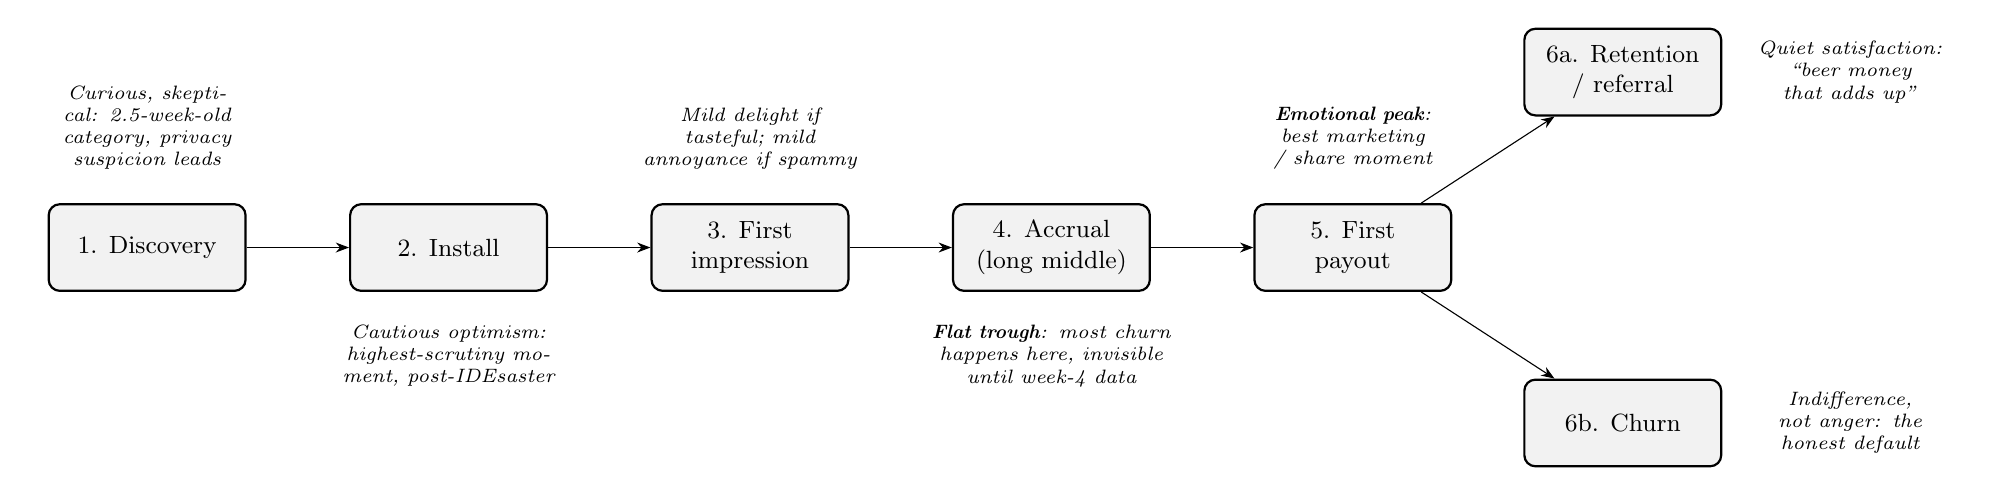
\begin{tikzpicture}[
    node distance = 1.3cm,
    stage/.style = {rectangle, rounded corners, draw=black, thick, fill=gray!10,
                     minimum width=2.5cm, minimum height=1.1cm, align=center, font=\small},
    emo/.style = {align=center, font=\scriptsize\itshape, text width=2.8cm},
    >=Stealth
]

% --- Stage nodes (horizontal sequence) ---
\node[stage] (disc) {1. Discovery};
\node[stage, right=of disc] (inst) {2. Install};
\node[stage, right=of inst] (first) {3. First\\impression};
\node[stage, right=of first] (accrue) {4. Accrual\\(long middle)};
\node[stage, right=of accrue] (payout) {5. First\\payout};
\node[stage, above right=1.1cm and 0.9cm of payout] (retain) {6a. Retention\\/ referral};
\node[stage, below right=1.1cm and 0.9cm of payout] (churn) {6b. Churn};

% --- Arrows along the main sequence ---
\draw[->] (disc) -- (inst);
\draw[->] (inst) -- (first);
\draw[->] (first) -- (accrue);
\draw[->] (accrue) -- (payout);
\draw[->] (payout) -- (retain);
\draw[->] (payout) -- (churn);

% --- Emotional annotations above/below each node ---
\node[emo, above=0.3cm of disc] {Curious, skeptical: 2.5-week-old category, privacy suspicion leads};
\node[emo, below=0.3cm of inst] {Cautious optimism: highest-scrutiny moment, post-IDEsaster};
\node[emo, above=0.3cm of first] {Mild delight if tasteful; mild annoyance if spammy};
\node[emo, below=0.3cm of accrue, text width=3.1cm] {\textbf{Flat trough}: most churn happens here, invisible until week-4 data};
\node[emo, above=0.3cm of payout, text width=3cm] {\textbf{Emotional peak}: best marketing / share moment};
\node[emo, right=0.2cm of retain, text width=2.6cm] {Quiet satisfaction: ``beer money that adds up''};
\node[emo, right=0.2cm of churn, text width=2.6cm] {Indifference, not anger: the honest default};

\end{tikzpicture}
\caption{Developer journey map: six stages from discovery to the retention/churn fork, with emotional state and design implication annotated at each stage (Section~\ref{sec:journey-map}).}
\label{fig:journey-map}
\end{figure}

\begin{table}[htbp]
\centering
\small
\begin{tabular}{@{}p{2.1cm}p{4.6cm}p{2.6cm}p{4.6cm}@{}}
\toprule
\textbf{Stage} & \textbf{What happens} & \textbf{Emotional state} & \textbf{Risk / design implication} \\
\midrule
1. Discovery & Sees a launch post / tweet / friend share / referral code, likely framed as ``the one that actually pays Indian devs'' \cite{mvpspec_2026}. & Curious, slightly skeptical. Category is 2.5 weeks old; loudest prior reaction was privacy suspicion, not excitement \cite{masterplan_2026}. & Landing page must lead with trust signals (source-available client, ``never reads your code'') \emph{before} the earnings pitch, or skepticism wins before curiosity does. \\
\addlinespace
2. Install & Installs the client; OAuth sign-in via Google/GitHub \cite{mvpspec_2026}. & Cautiously optimistic --- the highest-scrutiny moment. Deciding whether to trust a tool that touches the editor, right after the ``IDEsaster'' wave and a real supply-chain attack on dev tooling \cite{masterplan_2026}. & One-click disable visible immediately; the ``never reads code'' guarantee must be checkable, not asserted (open client or published data-flow disclosure). \\
\addlinespace
3. First impression seen & Sponsor line appears in the thinking status line for the first time, $\geq$5 seconds \cite{masterplan_2026}; status bar ticks balance up live. & Mild delight if native and tasteful; mild annoyance if spammy, irrelevant, or jarring. & First creative shown should be a curated house ad (Tier 0), not a rough early-advertiser creative --- first impressions of ``first impression'' matter disproportionately. \\
\addlinespace
4. Accrual (long middle) & Days to weeks of small balance increases (\textasciitilde\textrupee3.5--17/day at realistic usage, \cite{mvpspec_2026}). No payout yet. & The most fragile stretch --- flat, easy to forget. Nothing dramatic happens; novelty wears off here for most users. & Balance visibility (today/month/lifetime) and possibly streak/bonus mechanics \cite{mvpspec_2026} must do real work --- most churn happens here, invisible until week-4 data lands. \\
\addlinespace
5. First payout & Balance crosses \textrupee300; RazorpayX UPI payout fires automatically; developer gets a UPI notification with real rupees from Devorix. & The single highest emotional peak. ``Real money landed from an AI coding tool'' is the believable, shareable moment. & Instrument this for shareability (prompt to screenshot / share / refer). The one moment that converts a quiet user into a public advocate. \\
\addlinespace
6a. Retention / referral & Keeps the client past novelty, maybe refers friends, checks balance periodically. & Quiet satisfaction --- ``beer money that adds up'' \cite{mvpspec_2026}. Not a daily-delight product. & Week-4 retention is \emph{the} most important open question \cite{masterplan_2026} --- instrument cohorts explicitly, not just gross install counts. \\
\addlinespace
6b. Churn (honest default) & Novelty fades before \textrupee300, or the developer forgets/uninstalls; content feels stale; no meaningful balance noticed. & Indifference, not anger --- the more likely failure mode \cite{masterplan_2026}. & Plan for this as the base case. Make the rare ``ah right, I have this'' re-engagement moment (a payout notification) count for as much as possible. \\
\bottomrule
\end{tabular}
\caption{Developer journey map detail: stage, behavior, emotional state, and design implication.}
\label{tab:journey-detail}
\end{table}

\clearpage
\section{Cross-Cutting Trust Findings (Must Be Addressed Head-On)}
\label{sec:trust-findings}

Three findings cut across every persona and journey stage. The first two are \textbf{elevated, newly-surfaced risks} that this chapter flags clearly for the risk-analysis chapter (Devorix does not own that chapter but must not let these get lost).

\begin{enumerate}
\item \textbf{Anthropic has publicly branded itself the anti-ads AI.} Anthropic ran satirical Super Bowl LX ads (February 2026) --- titled ``Deception,'' ``Betrayal,'' ``Treachery,'' ``Violation'' --- jabbing at OpenAI's plan to put ads in ChatGPT, under the tagline \textbf{``Ads are coming to AI. But not to Claude.''} Its leadership's stated rationale: ads could undermine user trust in conversational AI (\emph{Verified fact} \cite{anthropic_antiads_fortune_2026,anthropic_antiads_techcrunch_2026,anthropic_antiads_cnbc_2026}). Kickbacks launched approximately four months later. \textbf{The platform owner of Devorix's first target tool has aggressively positioned itself against the exact thing Devorix monetizes.} Devorix's non-patching architecture mitigates the \emph{technical/ToS} risk \cite{masterplan_2026} but does \textbf{not} erase the \emph{brand-perception} tension. Casual observers will conflate ``a third-party status-bar tool sponsored alongside Claude Code'' with ``ads inside Claude.'' The PRD must make the distinction explicitly and repeatedly: \emph{Devorix never advertises inside Claude's responses; it sponsors a third-party status line that sits outside Anthropic's control.}

\item \textbf{IdleAds already claims the identical trust positioning Devorix planned to own.} IdleAds' own launch framing is ``Impressions are verified server-side, the editor is never patched, and the CLI never sees your code or prompts'' (\emph{Verified fact} \cite{idleads_showhn_2026}). That is the same trust/architecture axis Devorix is betting on. \textbf{Devorix's trust positioning is therefore not novel --- a live competitor makes the identical claim with no more proof than Devorix currently has.} The differentiation must come from \emph{proven} trust (open client, real India UPI payout execution, real advertiser renewals), not from claiming a posture nobody else has claimed. This sharpens, rather than changes, the existing read that the moat is execution depth \cite{masterplan_2026}.

\item \textbf{The ``ads in developer tooling'' backlash precedent is real but mechanically distinct.} In 2019, \texttt{npm install funding} printed a sponsor line on every npm install; backlash was immediate (``adware is malware''), ad-blockers appeared within a week, Linode pulled out, and npm banned ad-displaying packages platform-wide (\emph{Verified fact} \cite{npm_funding_infoq_2026,npm_funding_register_2026,npm_funding_hn_2026}). The precedent is citable, but the trigger was an \emph{unavoidable, repeated, non-opted-into} ad on a core automated command with no value to the installer. Devorix's developer is a \textbf{willing, compensated participant from install} --- a load-bearing difference the PRD should state, while still treating the backlash pattern as a live risk. Also relevant: a comment plugging IdleAds inside the Kickbacks HN thread was traced to IdleAds' own founder --- first-degree astroturfing in a category barely 24 hours old. Devorix marketing must avoid even the appearance of this; the audience is small and incestuous.
\end{enumerate}

\section{Figures Needed (Chapter 4)}
\label{sec:ch4-figures}

\begin{itemize}
\item \textbf{Two-sided customer map} --- developer (publisher) side and advertiser side of the same transaction, with the 50/50 split in the middle and ``attention pool, not pain point'' annotation.
\item \textbf{Persona one-pagers (\texttimes5)} --- realized above in Section~\ref{sec:developer-personas} and Section~\ref{sec:advertiser-personas} as bordered tables; each carries a single ``key evidence'' callout (GitHub Sponsors 60\%-unpaid stat for Rohit; credits-beat-cash \textasciitilde18\% for Ananya; data-egress-is-top-concern for Vikram; EthicalAds \$2.50 CPM parity for Priya; GST-INR-invoice wedge for Karthik).
\item \textbf{Developer journey map} --- realized above as Figure~\ref{fig:journey-map} and Table~\ref{tab:journey-detail}: six stages plotted with emotional annotation, marking the accrual trough as ``where most churn actually happens'' and the first-payout peak as ``best marketing asset / share moment.''
\item \textbf{Advertiser objection-to-resolution matrix} --- top objections (fraud/real impressions, price-vs-Carbon, clone longevity, brand safety, audience size) mapped to the proof artifact that resolves each (honest ranged report, captive-attention framing, renewal story, curated house creative, ``test budget not channel commitment''); see Persona~4--5 objection rows in Section~\ref{sec:advertiser-personas} for the underlying content, to be rendered as a matrix table in the design pass.
\end{itemize}

\chapter{Business Strategy: Model, Positioning, and Moats}
\label{chap:business-strategy}

\section{Investor-Thesis Anchors}
\label{sec:thesis-anchors}

Before describing the business model in detail, it is worth grounding Devorix's pitch in the funding environment it sits inside. The anchors below are real, citable fund signals, each labeled with whether Devorix actually fits the thesis being cited -- overclaiming category fit is a credibility risk we deliberately avoid here.

\begin{itemize}
  \item \textbf{Lightspeed / Paid (paid.ai), Sep 2025 --- \$21M seed.} Framed by Lightspeed as ``the missing economic infrastructure for AI agents,'' with the next wave of AI value coming from infrastructure that operationalizes AI deployment at scale \textbf{(Verified fact)} \cite{paidai_2025}. \textit{Fit:} thesis-adjacent only. Paid prices agent \emph{output} for B2B AI vendors; Devorix monetizes idle attention in human-supervised coding. The honest reading is ``monetization infrastructure for the agent economy is a fundable category to a top-tier fund,'' not a direct comp -- and Paid had a repeat founder, a working product, and a \$21M seed, where Devorix is solo, pre-advertiser, and pre-user.
  \item \textbf{Sequoia, 2026 thesis.} Roughly 60\% of capital deployed since 2025 has gone into AI apps and infrastructure -- Sequoia's most concentrated thematic bet since the cloud era -- with named clusters in foundation-model infrastructure (OpenAI, Stripe) and workflow-owning vertical agents (Harvey, Sierra, Glean) \textbf{(Verified fact)} \cite{sequoia_2026}. \textit{Fit:} Devorix fits none of the three named clusters. The honest framing is ``monetization-layer infrastructure adjacent to a fast-growing agent surface (Claude Code),'' not ``we are an agent company.''
  \item \textbf{Peak XV (ex-Sequoia India), Feb 2026 --- \$1.3B fund, India-weighted}, with named priority verticals including developer tooling, vertical SaaS, and regulated fintech \textbf{(Verified fact)} \cite{peakxv_2026}. \textit{Fit:} the strongest direct support found for India-first sequencing -- a named top India fund's current deployment focus, not an inferred argument. Peak XV and Lightspeed have also co-led a \$200M Series B in Sarvam AI, evidence the two relevant funds actively co-invest in Indian AI infrastructure.
  \item \textbf{YC cold-start doctrine} -- ``do things that don't scale,'' founder-led manual recruitment of the hard side of a marketplace, as in early Airbnb \textbf{(Verified fact, general essay corpus)} \cite{ycombinator_coldstart}. \textit{Fit:} validates the Days 1--3 hand-sold advertiser motion described in Section~\ref{sec:gtm-overview} of the GTM chapter as canonical practice, not an improvisation.
  \item \textbf{Accel --- honestly flagged gap.} No Accel-specific or named-partner 2025--2026 quote on this category was found. \textbf{Internal assumption:} Accel's general SaaS/marketplace thesis is consistent with, but not specifically about, Devorix. We do not present Accel as having endorsed the category.
\end{itemize}

\textbf{Stage verdict (preserved, unsoftened):} this is a \emph{pre-seed / accelerator-stage story, not a seed story} -- solo founder, pre-revenue, zero advertisers, zero installs, a ₹1-lakh budget. The honest ask is ``give us a small check or an accelerator slot to prove the loop,'' not ``fund the billion-dollar vision.''

\section{The Business Model}
\label{sec:business-model}

Devorix's mechanic, locked per MASTER-PLAN \S2, is an ads-to-developers model: when an AI coding tool such as Claude Code is in a ``thinking'' wait-state, Devorix renders a small, tasteful sponsor line in that otherwise-wasted status bar, and shares the resulting revenue with the developer, paid in rupees over UPI. The model is non-patching and status-bar only -- the client never touches Claude Code's rendering layer or OAuth tokens, and never reads the developer's code.

\subsection{Revenue split and pricing ladder}

The developer revenue share is locked at \textbf{50/50} (MASTER-PLAN decision \#11, \textbf{DECIDED FINAL}), and the payout threshold is locked at \textbf{₹300} (decision \#13). The live FX reference used throughout this PRD is \textbf{₹94/USD} (decision \#16, re-verified 2026-06-28).

Pricing follows a deliberately staged hybrid ladder (MASTER-PLAN \S5.1, decision \#14) rather than a single mechanism chosen up front:

\begin{table}[htbp]
\centering
\caption{The hybrid pricing ladder}
\label{tab:pricing-ladder}
\begin{tabular}{@{}p{1.6cm}p{2.6cm}p{5.2cm}p{4.2cm}@{}}
\toprule
\textbf{Tier} & \textbf{Activates when} & \textbf{How it sells} & \textbf{What is built} \\
\midrule
Tier 0 & Launch $\rightarrow$ \textasciitilde5 advertisers & Flat monthly sponsorships, ₹10{,}000--15{,}000/mo (``exclusive sponsor line to N active Indian developers''); not CPM, since CPM math at $<$500 devs yields \textasciitilde₹12/dev/mo, unsellable. & House-ad serving engine + manual flat-deal creative rotation. No rate card, no self-serve. \\
Tier 1 & 5--10 advertisers signed & Publish the reconciled CPM rate card (\$2--3 India / \$5--8 Global, both tagged \emph{Internal assumption}) and sell blocks against it; flat deals continue as an enterprise upsell. & Fixed-price block-serving engine -- this is when the system starts handling real recurring revenue, not just existing structurally. \\
Tier 2 & 5{,}000+ DAU & Real-time second-price auction. & Built only once supply-side liquidity is large enough for bids to be meaningful. \\
\bottomrule
\end{tabular}
\end{table}

In practice today: 1 advertiser = ₹15,000/mo; 2--3 advertisers = ₹30,000--45,000/mo; at 100--500 installs each developer nets roughly ₹100--190/month \textbf{(Internal assumption, MASTER-PLAN \S5.2)}. The model stays cash-positive from month 1 because operating costs are tiny (\textasciitilde₹5,000/month all-in).

\subsection{Pricing rationale}

The Tier-1 CPM band (\$2--3 India, \$5--8 Global) is deliberately anchored to the only independently audited real number anywhere in developer advertising -- Carbon Ads' verified \$1.60 effective CPM over three years, selling to funded, trusted brands (Okta, GitLab, MongoDB) on a decade-old network \textbf{(Verified fact)} \cite{pragmaticengineer_carbonads_2024}. Competing internal estimates from earlier planning documents proposed \$8--15 CPM, three to ten times that audited number; charging five to ten times what a trusted incumbent charges, before Devorix has proven anything, is a guaranteed objection on every cold pitch. The reconciled \$2--3 band represents roughly 1.3--2x Carbon's number, justified by the captive, full-attention nature of a wait-state spinner versus a passive sidebar a user scrolls past, while staying within hailing distance of the only real comp rather than far beyond it. This is tagged \textbf{Internal assumption -- revisit immediately once Tier 1 has real fill data} (MASTER-PLAN \S5.4).

The billable impression length is set at \textbf{5 seconds} for the v1 build (decision \#15), matching category convention (Kickbacks, IdleAds) and the existing technical spec, with 10 seconds retained as a documented, data-gated option pending real telemetry on Claude Code thinking-state durations.

\section{Competitive Positioning}
\label{sec:competitive-positioning}

\begin{table}[htbp]
\centering
\caption{Competitive positioning matrix}
\label{tab:competitive-positioning}
\begin{tabular}{@{}p{2.6cm}p{2.6cm}p{2.6cm}p{2.6cm}p{2.8cm}@{}}
\toprule
\textbf{Dimension} & \textbf{Devorix} & \textbf{Kickbacks} & \textbf{IdleAds} & \textbf{Carbon Ads} \\
\midrule
Dev rev-share & 50/50 (locked) & 50\% & 70\% (90\% goal) & n/a (publisher network) \\
Architecture & Non-patching, status-bar only, never reads code & Patches Claude rendering layer (ToS risk) & UPI manual & Sidebar display \\
Payout rail & Native automated UPI (RazorpayX), GST-ready & Stripe Connect (India-blocked, not live as of Jun 2026) & Manual UPI & n/a \\
India focus & India-first, native & Global, India-blocked & Some India & Global \\
Trust positioning & ``Non-patching, never reads your code,'' verifiable & --- & Already claims the same trust positioning (collision) & Mature trusted network \\
Verified paying advertisers & 0 (category-wide) & 0 & 0 & Okta/GitLab/MongoDB (audited \$1.60 CPM) \\
\bottomrule
\end{tabular}
\end{table}

\textbf{(Verified fact for all rows; see \cite{kickbacks_2026, idleads_2026, pragmaticengineer_carbonads_2024}.)} Devorix's architectural and payout-rail advantages are real and citable. They are not yet proven moats -- see Section~\ref{sec:moats}.

\section{Moats and Defensibility}
\label{sec:moats}

\textbf{Devorix has no strong moat today.} This verdict is deliberate, and it is not softened in this synthesis.

\begin{itemize}
  \item \textbf{Network effects: none today, on either side.} A developer installing the client does not change the value of the product for the next developer -- there is no dev-to-dev network effect. ``More developers = bigger reach'' is a \emph{scale} effect (linear, sellable to advertisers), not a network effect, and conflating the two is a classic pre-seed overclaim that an experienced investor will discount on sight. A mild data-network-effect could emerge once the Tier-2 auction reaches liquidity (Month 12--18) -- flagged here as upside, not underwritten.
  \item \textbf{Switching costs: weak on both sides.} Uninstalling a status-bar overlay is trivial. The 50/50-vs-70\% gap versus IdleAds gives developers a legible, rational reason to prefer the competitor, offset only by an as-yet-unproven trust/UX/India-payout-reliability advantage. The advertiser side carries only normal vendor friction, not a structural lock-in -- it evaporates on one bad report.
  \item \textbf{Data/targeting: none today} -- Tier 0 pricing is flat and undifferentiated. This is the single most legitimate ``moat in the making,'' but it requires deliberate attribution/ledger investment starting now, and realistically 12+ months before it becomes real.
  \item \textbf{Brand/trust: the best near-term candidate, and the most fragile.} Concrete assets already exist: a verifiable non-patching architecture (a real, citable differentiator versus Kickbacks); reliable UPI-native payouts (a genuine advantage for an India audience that has been burned by foreign-platform promises while Stripe stays blocked); and honest earnings-range messaging against a category full of inflated \$8--42 self-reported CPM claims. But none of this is \emph{brand} yet -- it is a set of good decisions that could compound into trust over 6--12 months of clean execution. Trust is also copyable in principle, and the edge is being first to actually prove it over time, which is a time-based advantage, not a structural one. IdleAds already claims the identical trust positioning (see the Risk Register, Chapter~\ref{chap:risk-analysis}, risk R4), so even this candidate is contested.
\end{itemize}

\textbf{The structural reason the mechanic itself cannot be the moat: multi-homing.} \textbf{(Verified fact, marketplace-defensibility literature)} \cite{chen_coldstart_2021}: multi-homing -- participants using competing platforms without penalty -- is the central structural weakness of marketplace moats, and nothing stops a developer or an advertiser from running Devorix and IdleAds or Kickbacks side by side. The same literature confirms that monetizing too early is one of the most damaging decisions a marketplace can make, which independently validates the staged hybrid ladder (Tier 0 $\rightarrow$ Tier 1 at 5--10 advertisers $\rightarrow$ Tier 2 at 5{,}000+ DAU) described in Section~\ref{sec:business-model}.

\textbf{Ranked moat candidates, in order of plausibility:} (1) trust/brand via consistent execution plus a verifiable non-patching architecture; (2) India payout-rail depth and compliance maturity; (3) data/targeting compounding. Network effects and switching costs are the weakest candidates and should not be leaned on in any investor conversation.

\section{Self-Critique}
\label{sec:self-critique}

Each axis below either defends the locked choice with explicit reasoning, or proposes a concrete, low-cost improvement. No locked decision (MASTER-PLAN \S2) is reopened.

\begin{itemize}
  \item \textbf{Business model --- defend, sharpen.} Ads-to-developers is the only structurally differentiated option given the constraints; a subscription or usage-based product would compete head-on with Anthropic and Cursor directly. \textit{Improvement:} define numerically what ``demand is real'' means -- renewal at the \emph{same or higher} price, not a begged discount. The current \S8.3 gate requires renewal but not renewal at full price; close that gap before Month 4.
  \item \textbf{Pricing --- defend the ladder, add a floor.} The Tier-0 ₹10,000--15,000/mo band is an untested founder anchor; the Tier-1 \$2--3 CPM figure is honestly tagged \emph{Assumption}. The real risk is having zero pricing power at 1--3 advertisers. \textit{Improvement:} institute a price-floor rule now -- never close below ₹8,000/mo even if it costs the deal -- to stop a panic-discounted first deal from anchoring every deal that follows. This is a zero-cost, meaningfully de-risking move.
  \item \textbf{Growth/GTM --- add a time-budget gate.} The plan silently assumes infinite solo-founder bandwidth through Month 4. \textit{Improvement:} if by Month 3 the founder is spending materially more time on developer support than on advertiser sales and relationship-deepening (the actual differentiator), treat that as a leading ``doesn't scale solo'' signal independent of revenue -- a self-check, not new infrastructure.
  \item \textbf{Tech/architecture --- defend unreservedly, verify cheaply.} Non-patching is the single best risk decision in the plan. But ``never reads your code'' is currently \emph{asserted}, not verified -- barely better than no claim at all in the current trust-suspicious climate. \textit{Improvement:} open-source the client (keeping the backend/ledger private), or publish a one-page data-flow document, as an explicit Days 3--10 sprint task. This converts an assertion into a checkable fact.
  \item \textbf{Positioning/narrative --- lead with advertiser pain.} The biggest narrative risk, already self-identified, is mixing a ``financial infrastructure for autonomous software'' long-range vision with a ``fund a 14-day sprint'' near-term ask. The fix is to frame the vision explicitly as long-range optionality, not the headline. Additionally, the Devorix rebrand (2026-06-28) is extremely recent and untested with either developers or advertisers -- one more unvalidated variable to track. \textit{Improvement:} lead the public and investor narrative with the advertiser-side pain (``dev-tool marketers have shockingly few high-trust placements'') -- the more defensible, less novelty-dependent story -- rather than the crowded developer-earnings hook that four competitors already run.
\end{itemize}

\section{Business Model Canvas}
\label{sec:bmc}

Figure~\ref{fig:bmc} lays out Devorix's business model using the standard nine-box Business Model Canvas, populated with the specifics above rather than generic placeholders.

\begin{figure}[htbp]
\centering
\resizebox{\textwidth}{!}{%
\begin{tikzpicture}[
  font=\scriptsize,
  box/.style={draw, align=left, text width=3.5cm, minimum height=4.4cm, inner sep=4pt, anchor=north west, font=\scriptsize},
  hdr/.style={font=\bfseries\scriptsize}
]
% Row heights and column widths chosen to mimic the classic BMC layout:
% Col widths: 3.5 / 3.5 / 3.5(tall, spans 2 rows) / 3.5 / 3.5  -- total ~17.5cm scaled down
% Row heights are sized generously (4.4cm/row) so that 4-5 lines of \scriptsize
% wrapped text never overflow a box's bottom edge into the row below --
% anchor=north west means a box only ever grows downward if content exceeds
% minimum height, so under-sizing the row height is what causes visual overlap.
% We lay it out as a grid using a matrix-like coordinate scheme.

% Top-left origin
\coordinate (O) at (0,0);

% Column x-positions
\def\cA{0}
\def\cB{3.6}
\def\cC{7.2}
\def\cD{10.8}
\def\cE{14.4}

% Row y-positions (top of each row)
\def\rTop{0}
\def\rMid{-4.6}
\def\rBottom{-9.2}

% Key Partners (spans 2 rows, left column)
\node[box, minimum height=9.2cm] (kp) at (\cA,\rTop) {
  \textbf{Key Partners}\\[2pt]
  RazorpayX (UPI payout rail, GST-ready)\\
  Anthropic / Claude Code ecosystem (host surface)\\
  Ring-1 dev-tool advertisers (Firecrawl-style, vector DBs, MCP tooling)\\
  Future: cloud DevRel (AWS/GCP/Azure), campus ambassador network
};

% Key Activities (top, col B)
\node[box] (ka) at (\cB,\rTop) {
  \textbf{Key Activities}\\[2pt]
  Cold advertiser outreach \& sales\\
  Non-patching client engineering\\
  Ledger / UPI payout operations\\
  Trust verification (data-flow doc / open-source client)
};

% Value Propositions (spans 2 rows, center)
\node[box, minimum height=9.2cm] (vp) at (\cC,\rTop) {
  \textbf{Value Propositions}\\[2pt]
  \textit{Devs:} earn real ₹ from idle ``thinking'' time, paid natively over UPI, 50/50 share\\[4pt]
  \textit{Advertisers:} a high-trust, captive placement in the agentic-coding moment that Carbon Ads doesn't serve\\[4pt]
  Non-patching, never-reads-your-code architecture
};

% Customer Relationships (top, col D)
\node[box] (cr) at (\cD,\rTop) {
  \textbf{Customer Relationships}\\[2pt]
  Hand-sold, founder-led advertiser accounts (high-touch, Tier 0/1)\\
  Self-serve install for devs\\
  Honest-earnings-range messaging (anti-hype)
};

% Customer Segments (spans 2 rows, right column)
\node[box, minimum height=9.2cm] (cs) at (\cE,\rTop) {
  \textbf{Customer Segments}\\[2pt]
  \textit{Supply side:} India-based Claude Code developers (27M India GitHub devs)\\[4pt]
  \textit{Demand side:} Ring 1 AI-infra/dev-tool sellers; Ring 2 India dev-economy sellers; Ring 3 global dev-tool brands (Phase 2)
};

% Key Resources (below Key Activities)
\node[box] (kr) at (\cB,\rMid) {
  \textbf{Key Resources}\\[2pt]
  Founder time (solo, ₹1-lakh budget)\\
  AI Studio prototype (landing page / proof)\\
  RazorpayX integration\\
  Devorix brand \& domain (devorix.ai)
};

% Channels (below Customer Relationships)
\node[box] (ch) at (\cD,\rMid) {
  \textbf{Channels}\\[2pt]
  Cold DM / outreach (advertisers)\\
  Launch tweet / X (proven in-category viral channel)\\
  GitHub ecosystem placement\\
  Campus ambassadors (Month 9--12)
};

% Cost Structure (bottom row, spans left 2.5 columns)
\node[box, minimum width=10.6cm, text width=10.2cm, minimum height=2.6cm] (costs) at (\cA,\rBottom) {
  \textbf{Cost Structure}\\[2pt]
  Near-zero infra/hosting (\textasciitilde₹5,000/month all-in) · solo-founder opportunity cost · RazorpayX payout fees · micro-influencer/launch budget (\textasciitilde₹45,000--75,000 one-time)
};

% Revenue Streams (bottom row, spans right 2 columns)
\node[box, minimum width=7.0cm, text width=6.6cm, minimum height=2.6cm] (rev) at (\cD,\rBottom) {
  \textbf{Revenue Streams}\\[2pt]
  Tier 0: flat monthly sponsorships (₹10,000--15,000/mo)\\
  Tier 1: CPM rate card (\$2--3 India / \$5--8 Global)\\
  Tier 2: real-time auction (5{,}000+ DAU)\\
  All split 50/50 with developers
};

\end{tikzpicture}%
}
\caption{Devorix Business Model Canvas}
\label{fig:bmc}
\end{figure}

\section{Value Proposition Canvas}
\label{sec:vpc}

Figure~\ref{fig:vpc} expands the developer-side value proposition (the supply side of the marketplace) into the standard jobs/pains/gains versus products-pain-relievers-gain-creators structure, shown as a $2\times2$ grid.

\begin{figure}[htbp]
\centering
\resizebox{\textwidth}{!}{%
\begin{tikzpicture}[
  font=\scriptsize,
  quad/.style={draw, text width=6.6cm, align=left, minimum height=8.4cm, inner sep=6pt, anchor=north west, font=\scriptsize},
  fitquad/.style={draw, text width=6.6cm, align=left, minimum height=4.6cm, inner sep=6pt, anchor=north west, font=\scriptsize},
  hdr/.style={font=\bfseries\small}
]
% Top row (cp/vm) gets a taller minimum height (8.4cm) than the bottom row
% (4.6cm, via fitquad) because each top box carries three dense paragraphs;
% the row gap below (rows start 8.8cm apart) is sized to clear that content
% so anchor=north west growth never spills into the fit-check row.
\node[quad] (cp) at (0,0) {
  \textbf{Customer Profile --- Developer Jobs}\\[2pt]
  \textit{Jobs:} ship code with Claude Code; wait through ``thinking'' states multiple times per session\\[4pt]
  \textit{Pains:} idle wait-time produces zero value; existing wait-state ad tools (Kickbacks) patch the rendering layer and raise privacy/ToS concerns; IdleAds offers a higher 70\% rev-share\\[4pt]
  \textit{Gains sought:} extra income with zero behavior change; payouts that actually land in India (UPI, not blocked Stripe); confidence the tool never reads code
};
\node[quad] (vm) at (7.2,0) {
  \textbf{Value Map --- Devorix Offer}\\[2pt]
  \textit{Products/services:} status-bar sponsor-line client; RazorpayX UPI payout (₹300 threshold, accrue-then-pay)\\[4pt]
  \textit{Pain relievers:} non-patching architecture (never touches OAuth tokens or rendering layer); honest earnings-range messaging instead of inflated \$8--42 CPM claims; verifiable (open-source / data-flow doc) ``never reads your code'' claim\\[4pt]
  \textit{Gain creators:} 50/50 split paid natively in ₹ over UPI, GST-ready; first mover on India-native automated payout while Stripe stays blocked for IdleAds/Kickbacks
};
\node[fitquad] (fit1) at (0,-8.8) {
  \textbf{Fit check --- where it holds}\\[2pt]
  India payout reliability directly relieves the \#1 structural pain (Stripe-India block) that even the rev-share leader (IdleAds) has not solved with automation.\\[4pt]
  Verifiable non-patching claim directly answers the trust/privacy pain that is the loudest reaction in the category (cf. Kickbacks' Show HN: privacy concern, not excitement).
};
\node[fitquad] (fit2) at (7.2,-8.8) {
  \textbf{Fit check --- where it does not (yet)}\\[2pt]
  50/50 share does \emph{not} relieve the rev-share pain versus IdleAds' 70\%/90\%-goal offer -- this gap is openly conceded, not papered over (Risk R2, Chapter~\ref{chap:risk-analysis}).\\[4pt]
  ``Never reads your code'' is currently asserted, not verified -- the gain/pain-reliever fit is conditional on shipping the verification (Section~\ref{sec:self-critique}).
};
\end{tikzpicture}%
}
\caption{Devorix Value Proposition Canvas (developer side)}
\label{fig:vpc}
\end{figure}

\chapter{Product Requirements}
\label{chap:product-requirements}

All requirements are grounded in \cite{mvpspec_2026}, \cite{prd_2026}, and the locked decisions in \cite{masterplan_2026}. None introduces a new locked decision; this chapter operationalizes existing ones.

\textbf{Locked facts this chapter builds on:} developer revenue share 50/50; payout threshold \textrupee300; pricing ladder Tier 0 (flat \textrupee10--15k/mo) $\to$ Tier 1 (CPM rate card, \$2--3 India / \$5--8 Global) $\to$ Tier 2 (auction, 5{,}000+ DAU); 5-second billable impression for v1; India-first, Global explicit Phase 2; client non-patching/status-bar, never reads code, never patches the renderer (\cite{masterplan_2026}).

\section{Functional Requirements --- v1}
\label{sec:functional-requirements}

\subsection{Client (VS Code + Claude Code, non-patching / status-bar)}

\begin{description}
\item[FR-1.] The client SHALL inject exactly one sponsored line into Claude Code's thinking status-line/spinner slot via the configurable \texttt{statusLine} mechanism in \texttt{\textasciitilde/.claude/settings.json} --- never by patching Claude Code's rendering layer \cite{mvpspec_2026,masterplan_2026}.
\item[FR-2.] The client SHALL prefetch and locally cache a small batch of approved creatives (text-only at v1: one short line + optional click URL) so the slot can render when briefly offline \cite{mvpspec_2026}.
\item[FR-3.] The client SHALL count a billable impression only when a creative has displayed continuously for $\geq$5 seconds \cite{masterplan_2026} with the tool in an active session state; it SHALL count a click when the optional click URL is opened.
\item[FR-4.] The client SHALL batch-report impression/click events (\textasciitilde every 60 seconds or 50 events, whichever first) to the backend, signed with a per-device/session token and tagged with a per-event idempotency key \cite{mvpspec_2026}.
\item[FR-5.] The client SHALL display a live status-bar balance (today / month / lifetime) sourced from the backend ledger, not computed client-side \cite{mvpspec_2026,prd_2026}.
\item[FR-6.] The client SHALL provide a single, immediately discoverable one-click control to disable sponsorship and restore the original spinner/status line, fully reversible with no residual state \cite{mvpspec_2026,prd_2026}.
\item[FR-7.] The client SHALL authenticate developers via Google or GitHub OAuth before activating any sponsor line or accruing balance \cite{mvpspec_2026}.
\item[FR-8.] The client SHALL NOT read, transmit, log, or cache source code, prompts, completions, file paths, or transcripts under any circumstance --- a hard architectural guarantee, not a configurable setting \cite{mvpspec_2026,prd_2026}. \emph{This requirement is what directly answers Vikram's existential confidentiality concern and the category's documented top fear, data egress (Chapter~\ref{chap:customer-research}, Sections~\ref{sec:developer-personas} and \ref{sec:trust-findings}).}
\end{description}

\subsection{Backend}

\begin{description}
\item[FR-9.] The Event Ingest API SHALL deduplicate every incoming event by event UUID + device + timestamp window, and SHALL apply server-side validity rules (minimum display time, max events/hour/device, plausible cadence, active-session signal) before any event is eligible to affect billing or payable balance \cite{mvpspec_2026}.
\item[FR-10.] The system SHALL maintain two separate stores: a high-write raw-event store and a Postgres double-entry ledger containing only fraud-filtered, billable/payable events. Advertisers are billed and developers are paid exclusively from the filtered ledger, never the raw store \cite{mvpspec_2026}.
\item[FR-11.] Ad Serving SHALL support Tier-0 house-ad rotation at launch (manually curated, no advertiser required) and SHALL support Tier-1 fixed-price block serving (1 block = 1{,}000 impressions, round-robin/weighted) once advertisers onboard --- both servable from the same engine without re-architecture \cite{mvpspec_2026,masterplan_2026}.
\item[FR-12.] Targeting at v1 SHALL be coarse only: geography (India) and optionally tool/editor --- no behavioral, code-content, or fine-grained demographic targeting \cite{mvpspec_2026}.
\item[FR-13.] The Publisher Dashboard SHALL show balance (today/month/lifetime), PAN/KYC capture and status, and payout settings \cite{mvpspec_2026,prd_2026}.
\item[FR-14.] The Advertiser onboarding flow MAY be manual/concierge at v1 (founder-operated) but SHALL still produce a GST-ready invoice artifact and a basic performance report (impressions, clicks, spend) per campaign \cite{mvpspec_2026,prd_2026}. \emph{The GST-ready INR invoice is Karthik's stated buying trigger and a core wedge vs.\ Stripe-based competitors (Chapter~\ref{chap:customer-research}, Section~\ref{sec:advertiser-personas}).}
\end{description}

\subsection{Payouts}

\begin{description}
\item[FR-15.] The system SHALL accrue earnings continuously but SHALL trigger a payout only when payable balance reaches or exceeds \textrupee300 \cite{masterplan_2026,mvpspec_2026}.
\item[FR-16.] Payouts SHALL execute via RazorpayX Payouts API to a developer's UPI VPA (preferred) or bank account (IMPS fallback), using a mandatory idempotency key per attempt, with webhook-driven status reconciliation (queued $\to$ processing $\to$ processed/failed/reversed) back into the ledger \cite{masterplan_2026,mvpspec_2026}.
\item[FR-17.] Payouts SHALL be gated on a valid PAN; the system SHALL collect PAN at or before first payout eligibility, regardless of current TDS applicability \cite{masterplan_2026,mvpspec_2026}.
\item[FR-18.] The accrued balance SHALL be modeled and described strictly as a payable (a debt Devorix owes, settled to a bank/UPI account), never as stored value the developer can load, spend, or hold in-product --- a regulatory boundary (RBI PPI rules), not a UX preference \cite{masterplan_2026}.
\end{description}

\section{Non-Functional Requirements --- v1}
\label{sec:nonfunctional-requirements}

\begin{description}
\item[NFR-1 (Fraud / trust integrity).] No event is eligible for billing or payout until it passes server-side fraud/validity filtering; the client is treated as untrusted/advisory at all times \cite{mvpspec_2026}. Existential, not optional --- ``if advertisers don't trust your impression counts, you have no business.'' This directly answers Priya's lead objection (Chapter~\ref{chap:customer-research}, Section~\ref{sec:advertiser-personas}).
\item[NFR-2 (Privacy / auditability).] The ``never reads your code'' guarantee MUST be independently verifiable --- via a source-available client or a published data-flow disclosure of exactly what leaves the device, not a marketing assertion \cite{masterplan_2026}. \emph{This is also the answer to finding \#2 in Chapter~\ref{chap:customer-research}, Section~\ref{sec:trust-findings}: IdleAds claims the same posture, so Devorix must prove it.}
\item[NFR-3 (Data residency).] Backend infrastructure SHALL be hosted in an India region (AWS/GCP Mumbai) for latency and DPDP Act 2023 data-residency alignment \cite{mvpspec_2026}.
\item[NFR-4 (Platform-policy safety).] The client SHALL remain non-patching at all times --- no modification of Claude Code's rendering layer, no extraction or reuse of Claude's own OAuth tokens --- to stay on the safe side of Anthropic's enforced Consumer Terms (\cite{masterplan_2026}, citing the January 2026 enforcement action \cite{anthropic_enforcement_2026}). A continuous engineering-discipline requirement, not a one-time decision. \emph{Note for the risk chapter: this controls the ToS/technical risk but not the Anthropic anti-ads brand-perception tension (Chapter~\ref{chap:customer-research}, Section~\ref{sec:trust-findings}, finding \#1), which is a positioning/comms risk, not an engineering one.}
\item[NFR-5 (Reliability of money movement).] Payout webhook reconciliation SHALL be idempotent and SHALL resolve all terminal states (processed/failed/reversed) back to ledger balance with no silent loss or double-payment \cite{mvpspec_2026}.
\item[NFR-6 (Reversibility).] Disabling the sponsor line SHALL take effect immediately and fully restore original tool behavior with no residual modification \cite{mvpspec_2026}.
\item[NFR-7 (Cost discipline).] Payout cost SHALL stay at \textasciitilde1\% or less of paid-out balance at the \textrupee300 threshold (RazorpayX UPI $\approx$ \textrupee2--5/payout) --- a designed property of the threshold choice, monitored as volume grows \cite{mvpspec_2026}.
\item[NFR-8 (Honest marketing claims).] Any earnings figures in-product or in marketing SHALL be presented as ranges with clearly labeled conservative defaults, never a single inflated per-impression number --- remediating the AI Studio prototype's \textrupee0.42/impression figure (implies a 4--7x-too-high eCPM vs.\ observed real data) \cite{prd_2026}. \emph{This is load-bearing for every developer install trigger in Chapter~\ref{chap:customer-research}, Section~\ref{sec:developer-personas} (trust > earnings number) and for Priya's fraud objection.}
\end{description}

\section{Future-State Requirements (Explicitly ``Future, Not v1'')}
\label{sec:future-requirements}

\emph{Activates once 5--10 advertisers are signed --- realistically beyond month 4 \cite{masterplan_2026}:}
\begin{description}
\item[FUT-1.] Publish a self-serve fixed-price CPM rate card (\$2--3 India / \$5--8 Global) and allow block purchase without founder concierge.
\item[FUT-2.] Self-serve advertiser portal: campaign creation, budget caps, creative upload, basic targeting, automated GST invoicing \cite{mvpspec_2026}.
\item[FUT-3.] Instrument and analyze real Claude Code thinking-state durations to data-drive a possible revisit of the 5s-vs-10s impression-length decision \cite{masterplan_2026} --- not to be acted on without real telemetry.
\end{description}

\emph{Activates at 5{,}000+ DAU \cite{masterplan_2026}:}
\begin{description}
\item[FUT-4.] Real-time second-price auction ad serving, alongside (not necessarily instead of) flat enterprise sponsorship deals.
\end{description}

\emph{Global Phase 2, gated on the go/no-go criteria in \cite{masterplan_2026}:}
\begin{description}
\item[FUT-5.] International payout rails (PayPal/Wise) and non-India advertiser GTM. Explicitly out of scope until the India gate clears.
\end{description}

\emph{Adopted from the AI Studio prototype, P1/P2 \cite{masterplan_2026} --- must never be a dependency of core ad-serving/ledger:}
\begin{description}
\item[FUT-6.] Ad-Copy Generator (Gemini): advertiser input $\to$ 3 sponsorship-line variations, as a cold-start onboarding aid (P1).
\item[FUT-7.] Wait-State Coach: lead-gen tool estimating idle time and earnings from usage inputs (P1).
\item[FUT-8.] Workspace Analyzer: screenshot-based theme/placement suggestions (P2, nice-to-have).
\end{description}

\section{KPIs / OKRs}
\label{sec:kpis-okrs}

Framed around the founder's actual go/no-go gate \cite{masterplan_2026} --- (1) $\geq$2 advertisers paid \emph{and} renewed, (2) developers stick past novelty (week-4 retention), (3) founder still wants to run it --- not invented metrics.

\begin{table}[htbp]
\centering
\small
\begin{tabular}{@{}p{2.6cm}p{3.6cm}p{3.3cm}p{4cm}@{}}
\toprule
\textbf{Metric} & \textbf{Definition} & \textbf{v1 target / read} & \textbf{Why it matters} \\
\midrule
D7 retention & \% of installers still active (client enabled, $\geq$1 session) 7 days post-install & No committed target; first cohort data is the point of the 14-day sprint \cite{masterplan_2026} & Early signal on whether novelty alone sustains a week \\
\addlinespace
D30 / week-4 retention & \% still active 30 days post-install & Go/no-go criterion \#2 --- no fixed \%, but ``developers stick after novelty fades'' must be observably true & The single most important open question in the business \cite{masterplan_2026} \\
\addlinespace
Advertiser renewal rate & \% of Tier-0 advertisers who renew after the first 1-month pilot & Go/no-go criterion \#1: $\geq$2 advertisers paid \emph{and} renewed by month 4 & Proves the loop on the side that is the actual bottleneck \cite{masterplan_2026} \\
\addlinespace
Fill rate & \% of impression slots served a paid (non-house) ad & ``The most important [metric] early'' \cite{prd_2026} & Directly measures whether real advertiser demand exists --- the category's core unproven assumption \\
\addlinespace
Payout success rate & \% of payouts reaching \texttt{processed} on first attempt without manual intervention & Track from the first live payout onward; no fixed target in source & Payout reliability is a top-level success metric \cite{prd_2026} \\
\addlinespace
Fraud rate & \% of raw events rejected by server-side filtering before billing/payout eligibility & Track from day 1; no numeric target in source & Trust-integrity signal; existential per \cite{mvpspec_2026} \\
\addlinespace
Installs & Cumulative client installs & 100 $\to$ 250 $\to$ 400 $\to$ 500 (months 1--4) & Land-grab metric, explicitly secondary to advertiser proof \cite{masterplan_2026} \\
\addlinespace
Revenue / cumulative net & Gross advertiser revenue, and net of costs & \textrupee15k $\to$ \textrupee30k $\to$ \textrupee30k $\to$ \textrupee45k; cumulative net \textasciitilde\textrupee39{,}500 by month 4 & The explicit financial bar for continuing past month 4 \\
\bottomrule
\end{tabular}
\caption{KPIs / OKRs framed around the founder's go/no-go gate.}
\label{tab:kpis-okrs}
\end{table}

\section{Acceptance Criteria (Highest-Risk / Highest-Leverage Requirements)}
\label{sec:acceptance-criteria}

Selected because each gates trust, money-correctness, or the go/no-go decision itself.

\subsection*{FR-3 / FR-9 --- 5-second billable impression + server-side validity}
\begin{itemize}
\item Given a creative renders, when it stays continuously visible $\geq$5 seconds with the editor in an active/focused session, then exactly one billable impression is recorded.
\item Given a creative shows \textless5 seconds (a fast thinking cycle), when the session ends, then no billable impression is recorded (the raw display event may still be logged for telemetry).
\item Given an event arrives with a UUID already seen for that device in the dedup window, when processed, then it is discarded and increments no ledger balance.
\item Given a device exceeds max-events/hour, when further events arrive, then they are flagged, excluded from the billable ledger, and the fraud-rate counter increments.
\end{itemize}

\subsection*{FR-8 / NFR-2 --- never reads code; auditability}
\begin{itemize}
\item Given the client is running, when network traffic leaving the device is inspected, then no code, prompt, completion, file path, or transcript is present --- only impression/click telemetry (timestamps, device/session token, creative ID, display duration).
\item Given a security-conscious developer wants to verify this, when they look, then a published human-readable disclosure (or open client source) of exactly what leaves the device is available --- not just a marketing assertion.
\end{itemize}

\subsection*{FR-6 / NFR-6 --- one-click disable, fully reversible}
\begin{itemize}
\item Given a developer clicks ``disable sponsorship,'' when it completes, then the original status line/spinner is restored within the same session, no restart required.
\item Given sponsorship is disabled, when settings are reopened, then no residual sponsor config, cached creative, or partial state remains active.
\end{itemize}

\subsection*{FR-15 / FR-16 --- \textrupee300 payout threshold, RazorpayX UPI}
\begin{itemize}
\item Given filtered-ledger balance $\geq$ \textrupee300, when the next payout batch runs, then a payout is initiated via RazorpayX to the registered VPA/bank account with a unique idempotency key.
\item Given a webhook reports \texttt{processed}, when the ledger updates, then payable balance is debited by exactly the paid amount and a payout record with reconciliation timestamp is created.
\item Given a webhook reports \texttt{failed} or \texttt{reversed}, when the ledger updates, then payable balance is restored (not lost) and the developer is notified of retry.
\item Given no valid PAN, when balance reaches \textrupee300, then the payout is held pending and the developer is prompted to complete PAN/KYC --- funds are not forfeited.
\end{itemize}

\subsection*{FR-10 --- two-ledger separation}
\begin{itemize}
\item Given an event is in the raw store, when it has not passed fraud/validity filtering, then it must not appear in the double-entry ledger or affect any bill or balance.
\item Given an advertiser requests a report, when generated, then all impression/click counts are sourced exclusively from the filtered ledger, never the raw store.
\end{itemize}

\subsection*{FR-11 --- house ads $\to$ fixed-price, same engine}
\begin{itemize}
\item Given zero advertisers, when a billable slot is available, then a house-ad creative is served and the impression is recorded (at \textrupee0 advertiser cost) for telemetry/proof-of-loop.
\item Given an active fixed-price block campaign, when a slot is available, then the creative is served per round-robin/weighted rotation and the block balance decrements by exactly 1.
\item Given a block balance hits zero, when the next slot is available, then the creative stops serving and the slot falls back to house-ad rotation with no manual intervention.
\end{itemize}

\subsection*{NFR-8 --- honest, ranged earnings claims}
\begin{itemize}
\item Given any surface shows expected earnings, when displayed, then it is a range (not a point estimate) with an explicitly labeled conservative default, visually marked as an estimate.
\item Given real observed CPM/earnings data becomes available, when marketing copy is next updated, then the range is reconciled against real data, not left at launch-time guesses.
\end{itemize}

\section{Figures Needed (Chapter 6)}
\label{sec:ch6-figures}

\begin{itemize}
\item \textbf{System architecture / data flow} --- non-patching client $\to$ batched signed events $\to$ Event Ingest (dedup + validity) $\to$ split into raw-event store vs.\ filtered double-entry ledger $\to$ billing (advertisers) and payouts (RazorpayX UPI). Annotate the ``client is untrusted'' boundary and the ``never reads code'' data-flow (only telemetry leaves the device).
\item \textbf{Pricing/tier ladder} --- Tier 0 (flat \textrupee10--15k/mo, house+flat) $\to$ Tier 1 (CPM rate card \$2--3 India / \$5--8 Global, 5--10 advertisers) $\to$ Tier 2 (auction, 5{,}000+ DAU), with activation triggers on the X-axis and ``same serving engine across Tier 0$\to$1'' called out.
\item \textbf{Payout state machine} --- accrual $\to$ \textrupee300 threshold gate $\to$ PAN gate $\to$ RazorpayX payout $\to$ webhook states (queued $\to$ processing $\to$ processed/failed/reversed) with reconciliation arrows back to the ledger (failed/reversed restore balance).
\item \textbf{KPI dashboard mock} --- the go/no-go gate as the headline (2 renewed advertisers, week-4 retention, founder intent), with fill rate and fraud rate as the two trust-integrity gauges and the months 1--4 installs/revenue trajectory as the secondary land-grab line.
\item \textbf{Requirements-to-persona traceability matrix} --- rows = top FRs/NFRs, columns = the five personas (Chapter~\ref{chap:customer-research}), cells mark which persona concern each requirement answers (e.g., FR-8/NFR-2 $\to$ Vikram + Rohit; FR-14 $\to$ Karthik; NFR-1/NFR-8 $\to$ Priya).
\end{itemize}

\chapter{System Architecture}
\label{chap:system-architecture}

\begin{quote}
\textit{Source-of-truth note: every decision in this chapter is subordinate to \texttt{MASTER-PLAN.md} \S2 (locked decisions) and \texttt{00-MVP-spec.md} (the v1 technical spec). Nothing here re-opens a locked decision; it grounds the existing v1 design in real-world comparables and adds an explicitly-labelled future-state section. Each claim carries one of three labels --- \textbf{Verified fact} (independently confirmed against a primary source), \textbf{Industry estimate} (directionally supported but self-reported or synthesized), or \textbf{Internal assumption} (Devorix's own judgment call, not externally sourced).}
\end{quote}

\section{How to read this chapter}
\label{sec:how-to-read}

The architecture splits into two registers, and keeping them apart is deliberate. \textbf{Part 1 (\S\ref{sec:external-validation}--\S\ref{sec:v1-data-flow}) is what gets built} in the 14-day sprint and the 4-month plan: a solo founder, a ₹1 lakh budget, a weeks-not-months build with no on-call rotation and no advertiser self-serve (\texttt{MASTER-PLAN.md} \S2 rows 4/8, \S8.2). \textbf{Part 2 (\S\ref{sec:part2-future}) is future-state optionality} --- Tier 1 and Tier 2 --- gated on the triggers already locked in \texttt{MASTER-PLAN.md} \S5.1 and \S8.4, and written to be \textit{evaluated}, not funded, at this stage.

This separation is not cosmetic. \texttt{MASTER-PLAN.md} \S11's own VC-lens validation names the single most common way pre-seed pitches lose credibility: mixing infrastructure-scale ambition with a ``fund a 14-day sprint'' ask. The defensible long-term claim is not that Devorix will build a sophisticated ad-tech stack --- auctions, fraud ML, and analytics warehouses are well-understood, copyable technology once there is a reason to build them. The defensible claim is that \textbf{the ledger and payout discipline built correctly at v1 --- double-entry, raw/billable event separation, payable-not-wallet design --- is what lets Tier 1 and Tier 2 bolt on later without a rewrite}, and that discipline costs almost nothing extra to build right now while being expensive and risky to retrofit onto a live money system later.

\section{External validation: the architecture is not novel, and that is the point}
\label{sec:external-validation}

Before describing the build, it is worth establishing that Devorix's v1 design is not an invention --- it is convergence on the only proven pattern at this scale. This matters for an investor reading the technical risk: there is a working template.

\begin{itemize}
  \item \textbf{Verified fact} \citep{carbonads_about_2026} --- Carbon Ads, the most mature developer-focused ad network (900+ publisher sites since 2010), runs a centralized-sell / distributed-serve model: a thin client-side tag pulls one pre-approved creative from a central ad server; publishers do not run an auction or pick the ad. Ad unit is a fixed simple spec (130\texttimes{}100px image + \textless{}80 chars text), one creative per slot, no real-time bidding, no self-serve buying. Publisher payout is a 60\% revenue share, \textbf{accrued and batched monthly}.
  \item \textbf{Verified fact} \citep{ethicalads_pub_2026} --- EthicalAds is the only fully open-source ad network in the comp set; its production serving stack (Python/Django) is public, proving that open-sourcing the serving/client stack at small scale is both viable and a trust/marketing asset, not just an engineering nicety. Its targeting is content/geography-based only --- no cookies, no individual tracking, server-log IPs deleted within 10 days.
\end{itemize}

Both comps map structurally onto Devorix's spec: centralized creative approval, simple weighted/round-robin serving, no client-side bidding, coarse geo-only targeting, and accrue-and-batch payout (\texttt{00-MVP-spec.md} \S3--\S6). The only material difference is payout cadence --- Carbon and EthicalAds batch monthly; Devorix batches on a \textbf{₹300 balance threshold} (locked, \texttt{MASTER-PLAN.md} \S2 row 13), better UX for small/sporadic earners at the cost of running a balance-check job frequently rather than monthly.

This is a \textbf{confirmatory finding, not a course-correction}: Devorix follows the only proven small-scale dev-ad-network pattern rather than inventing one.

\section{V1 system overview}
\label{sec:v1-overview}

The system has three planes, and the most important architectural rule is that the \textbf{money ledger is strictly separated from impression ingestion} (\texttt{00-MVP-spec.md} \S2):

\begin{table}[htbp]
\centering
\caption{The three planes of the v1 system}
\label{tab:three-planes}
\begin{tabular}{p{0.16\textwidth} p{0.28\textwidth} p{0.46\textwidth}}
\toprule
\textbf{Plane} & \textbf{Runs where} & \textbf{Core responsibility} \\
\midrule
Client & Developer's machine & Inject the sponsor line, count impressions/clicks, batch-report signed events \\
Backend & India-region cloud (AWS/GCP Mumbai, for DPDP residency) & Ad serving, event ingest + fraud filter, double-entry ledger, dashboards \\
Payouts & Backend job + RazorpayX & Threshold-triggered UPI batch payout with webhook reconciliation \\
\bottomrule
\end{tabular}
\end{table}

See Figure~\ref{fig:v1-architecture} (v1 system architecture diagram).

\section{The client --- non-patching status-bar overlay}
\label{sec:client}

\begin{itemize}
  \item A small local agent plus a Claude Code status-line integration (\texttt{\textasciitilde{}/.claude/settings.json} \texttt{statusLine} hook), with a VS Code status-bar item as the secondary surface. v1 covers \textbf{Claude Code only}; a Cursor adapter is a Day 30--60 stretch goal (\texttt{00-MVP-spec.md} \S9), abstracted behind a per-tool \texttt{AdSlotProvider} interface so new tools are added without touching core.
  \item Responsibilities (\texttt{00-MVP-spec.md} \S3): prefetch a small batch of approved text creatives (one line, optional click URL, cached for brief-offline serving); render into the wait-state slot; \textbf{count an impression at \textgreater{}=5 seconds dwell} (locked, \texttt{MASTER-PLAN.md} \S2 row 15); count a click on URL open; batch-report events (\textasciitilde{}60s or 50-event batches) signed with a device/session token and an idempotency key per event; and provide one toggle that fully restores the original spinner.
  \item \textbf{Verified fact} \citep{kickbacks_faq_2026} --- Kickbacks' own published impression-validity gate uses the \textbf{same 5-second consecutive-display minimum} during an active, human-initiated AI wait-state. This is direct external confirmation that 5s is the category-standard billable threshold, not an arbitrary Devorix choice.
  \item \textbf{Hard constraint, load-bearing for the entire compliance story:} the client \textbf{never reads code, prompts, or completions, and never touches Claude's OAuth tokens or rendering layer.} This is what keeps Devorix on the safe side of Anthropic's January 2026 enforcement line (\texttt{MASTER-PLAN.md} \S10) and is the basis of the ``we are not Kickbacks'' positioning. \textbf{Verified fact} \citep{kickbacksgithub_2026} --- Kickbacks patches Claude Code's rendering layer directly, which is precisely the posture Anthropic acted against. Devorix's non-patching overlay is the citable differentiator.
  \item \textbf{Industry estimate} \citep{idlen_2026} --- A third competitor, Idlen.io, states it analyzes \texttt{package.json} \textbf{locally on-device} for ad relevance (nothing leaves the machine) and renders ads in \textbf{isolated webviews} to avoid editor-performance impact. These are more technically-specific privacy/architecture disclosures than either Kickbacks or IdleAds have published, and are a useful template: Devorix should phrase its ``never reads your code'' claim with comparable technical specificity (publish a source-available client, as EthicalAds does and Kickbacks did), not as a bare marketing assertion.
  \item \textbf{Anti-tamper principle:} client events are advisory from an untrusted source. The \textbf{backend, not the client, decides what is billable/payable} (\texttt{00-MVP-spec.md} \S3/\S5).
\end{itemize}

\section{The backend}
\label{sec:backend}

\subsection{Ad serving --- Tier 0 only}
\label{sec:ad-serving-tier0}

At v1, ad serving is deliberately \textit{not} a serving engine in any real sense. It is a small rotation of (a) house promo lines (to validate the pipe before any advertiser exists) and (b) 1--3 manually-loaded flat-deal creatives per signed advertiser (\texttt{MASTER-PLAN.md} \S5.1). Concretely: a single small table --- \texttt{(advertiser\_id, creative\_text, click\_url, active, start\_date, end\_date)} --- read on each ad-request and round-robined or weighted by simple priority. No bidding, no CPM math, no targeting beyond a hardcoded \texttt{geo = India} default.

This is \textbf{Internal assumption}-grade undersizing, and correct: \texttt{MASTER-PLAN.md} \S5.1 explicitly states Tier 0 has no rate card and no self-serve, and 1--3 advertisers do not justify more. A config table plus a human doing sales calls \textit{is} the Tier-0 ad-serving system.

\subsection{Event ingest and fraud filter}
\label{sec:event-ingest}

A single ingest endpoint accepts batched events keyed by idempotency UUID + device/session token + timestamp window. Before anything touches the ledger, a small server-side validity filter runs (\texttt{00-MVP-spec.md} \S3/\S5):

\begin{itemize}
  \item Idempotency + dedup per event.
  \item Minimum display time (5s); max-events-per-hour-per-device ceiling; plausible-cadence check.
  \item \textbf{Named daily/periodic per-device caps} as an explicit control (not left implicit in ``plausible cadence''). \textbf{Verified fact} \citep{kickbacks_faq_2026} --- Kickbacks uses named daily/periodic caps as a stated control; Devorix should adopt the same explicitness.
  \item \textbf{Salted one-way IP hashing for sybil/multi-account detection.} \textbf{Verified fact} \citep{kickbacks_faq_2026} --- Kickbacks stores only a salted, one-way hash of the IP (never the raw address) to compute accounts-per-network and networks-per-account ratios. This is a directly reusable pattern: it detects one person running many fake accounts while \textit{strengthening} the ``we don't store identifying data we don't need'' trust claim. Devorix should adopt it in v1.
\end{itemize}

\textbf{Verified fact} (synthesized from \citep{fraudlogix_2026, humansecurity_2026, atul4u_2026}) --- Industry best practice is \textbf{pre-credit filtering} (block suspicious impressions before they count toward billing) over post-hoc clawback, because clawing back money already paid to a developer or invoiced to an advertiser is reputationally costly in a trust-thin category. Devorix's single-slot, one-creative design also structurally eliminates the ad-stacking fraud vector entirely --- worth stating in the trust section.

\textbf{Internal assumption} --- At Devorix's near-term scale (100--500 installs, 1--3 advertisers, \texttt{MASTER-PLAN.md} \S8.3), \textbf{single-device self-fraud} (a developer scripting fake ``thinking'' states to farm impressions) is a more relevant threat than distributed bot farms. The v1 filter should weight toward implausible 24/7 cadence and no-corresponding-editor-activity signals, not distributed-botnet detection, which is the higher-cost problem Devorix does not yet have. This is a build-specific judgment call, not an external claim.

Raw events are written to a cheap append-only store --- at v1 simply a Postgres \texttt{raw\_events} table. \texttt{00-MVP-spec.md}'s ClickHouse/Redis-Streams suggestion is the \textit{target} shape once write volume justifies a second datastore, \textbf{not} a day-1 requirement for a pre-launch product with zero users.

\subsection{Ledger / balance tracking}
\label{sec:ledger}

Postgres, double-entry, source of truth for money --- non-negotiable even at tiny scale, because it is the one component that must survive an audit later.

\begin{itemize}
  \item \textbf{Verified fact} \citep{moderntreasury_2026, sdkfinance_2026} --- Standard pattern for accrue-then-payout systems: a double-entry ledger where the user's visible balance is always a \textit{derived read} (\texttt{SUM(credits) - SUM(debits)}), never a separately-stored mutable field that can drift from transaction history. Every economic event (an impression becoming billable, an advertiser invoice, a payout) posts as a balanced entry pair. This is exactly \texttt{00-MVP-spec.md} \S2's ``Postgres, double-entry, dev balance.''
  \item Two logical tables matter most: \texttt{billable\_events} (the subset of raw events that passed the fraud filter and are eligible to generate payable) and \texttt{dev\_balances} (accrued-but-unpaid amount per developer, at the locked 50/50 split). \textbf{Advertiser billing and developer payable both derive from the same filtered ledger, never from raw events} --- this is what makes the ``real, honest report'' promise to advertisers (\texttt{MASTER-PLAN.md} \S11) credible.
  \item \textbf{Verified fact} \citep{kickbacks_faq_2026} --- Kickbacks' enforcement language explicitly describes \textbf{voiding ledger entries} tied to fraud. This confirms competitors also use a ledger-entry model (not a simple balance field) so fraudulent credits can be surgically reversed --- reinforcing the double-entry design and Devorix's clawback capability as designed-in, not an afterthought.
  \item \textbf{Payable, not stored value.} No load/spend/hold capability is exposed to developers. This keeps the design outside RBI's PPI/wallet definition (\texttt{MASTER-PLAN.md} \S7.1) and must stay structurally true as the system grows. Note: RBI issued draft PPI Master Directions as recently as April 2026 --- confirm the ledger design with a fintech-savvy CA before scaling past MVP.
  \item \textbf{Verified fact} \citep{refgrow_2026} --- The decisive principle from affiliate/creator-payout systems: \textbf{decouple the internal earnings ledger from the payment rail.} The ledger decides \textit{who earned what and when it is payable}; the rail (RazorpayX) only decides \textit{who can legally receive funds under what KYC}. If the internal ledger drifts from the rail's settled state (failed webhooks, reversals), \textbf{the platform bears the financial difference.} This elevates webhook verification and reconciliation (\S\ref{sec:payout-flow}) from hygiene to a money-correctness, liability-bearing requirement.
  \item \textbf{Industry estimate} \citep{sdkfinancemulticurrency_2026} --- Multi-currency ledger support is standard fintech but \textbf{not needed for INR-only Phase 1}. Forward-compatible constraint: don't hardcode INR-only assumptions into the schema, even though Phase 1 is INR-only --- relevant only when Global Phase 2 activates (\texttt{MASTER-PLAN.md} \S8.1).
\end{itemize}

\subsection{Publisher (developer) dashboard}
\label{sec:publisher-dashboard}

Minimal: current balance (today/month/lifetime), payout settings (UPI VPA or bank), and PAN/KYC capture. No analytics, no creative preferences, no referral system at v1 --- those are retention features, not part of the money loop.

\subsection{Advertiser side (Tier 0)}
\label{sec:advertiser-tier0}

No dashboard at v1. Onboarding is manual/concierge: a signed IO (simple, low-complexity contract per \texttt{MASTER-PLAN.md} \S11), a flat monthly invoice (₹10,000--15,000/mo), creative text collected by email/call and entered directly into the \S\ref{sec:ad-serving-tier0} table. GST invoicing is \textbf{not} built --- unneeded below the ₹20L/yr threshold, triggered only if a specific advertiser demands a GST invoice (\texttt{MASTER-PLAN.md} \S7.1).

\section{The payout flow --- RazorpayX UPI}
\label{sec:payout-flow}

This flow is a product feature, not just plumbing: the first real UPI payout screenshot is called out in \texttt{MASTER-PLAN.md} \S8.2 as Devorix's single best marketing asset.

\begin{itemize}
  \item \textbf{Verified fact} \citep{razorpaypayouts_2026} --- The integration sequence is \textbf{Contact \textrightarrow{} Fund Account \textrightarrow{} Payout}, with a dedicated first-class endpoint for UPI/VPA payouts. Confirmed accurate against current docs; no correction to \texttt{00-MVP-spec.md} \S6 needed.
  \item Threshold batch job: when a developer's accrued \texttt{dev\_balances} crosses \textbf{₹300} (locked), trigger a payout with a mandatory idempotency key \textrightarrow{} consume status webhooks (queued \textrightarrow{} processing \textrightarrow{} processed/failed/reversed) \textrightarrow{} reconcile against the ledger, decrementing the payable balance \textbf{only on \texttt{processed}}.
\end{itemize}

\begin{tcolorbox}[colback=yellow!10,colframe=black!60,title=Must-build-v1 requirements (not future-phase),boxrule=0.8pt,arc=2pt]
Two build-checklist items the explorer research surfaced --- \textbf{both are must-build for v1, not future-phase}:

\begin{enumerate}
  \item \textbf{HMAC-SHA256 webhook signature verification.} \textbf{Verified fact} \citep{razorpaywebhooks_2026} --- Payout webhooks are signed via HMAC-SHA256 with a webhook secret in the \texttt{X-Razorpay-Signature} header and \textbf{must be validated on receipt before trusting the payload.} \texttt{00-MVP-spec.md} \S6 mentions consuming webhooks but does not call out signature verification. Per \S\ref{sec:ledger}'s liability principle, an unverified or spoofed webhook that desyncs the ledger from RazorpayX's settled state is a money-correctness bug Devorix is financially liable for --- so this is a \textbf{money-correctness requirement, not optional hardening.}
  \item \textbf{VPA Account Validation at onboarding time.} \textbf{Verified fact} \citep{razorpayvpa_2026} --- A dedicated Account Validation API confirms a VPA resolves to a real, named account; a composite API creates Contact + Fund Account + validates the VPA in one call. Razorpay's own best-practice docs recommend validating the Fund Account \textit{before} issuing a payout. Devorix must call validation when a developer first adds/changes their UPI VPA in the Publisher Dashboard --- \textbf{once at onboarding, not per-payout} (it is a billable call, so per-payout would waste cost), rather than relying on the payout silently failing for a bad VPA.
\end{enumerate}
\end{tcolorbox}

Supporting verified facts: PAN is collected at signup regardless of whether TDS currently attaches (it does not yet --- \S194H attaches only past ₹1 crore turnover, \texttt{MASTER-PLAN.md} \S7.1) \citep{razorpaykyc_2026} --- RazorpayX's KYC-demand right is contractually open-ended, not threshold-gated, so PAN is a day-one non-negotiable for every payee. KYC turnaround is typically \textbf{1--2 working days} \citep{creativenexus_2026} --- the Publisher Dashboard should set this expectation, not imply instant payout eligibility. UPI settles 24/7 instantly; the ₹5 lakh per-transaction cap is irrelevant at \textasciitilde{}₹300--500 payouts. The full flow is tested end-to-end in the RazorpayX sandbox before any live payout.

See Figure~\ref{fig:sequence-diagram} (impression-to-payout sequence diagram).

\section{V1 data flow and explicit non-scope}
\label{sec:v1-data-flow}

\subsection{Data flow}
\label{sec:data-flow}

\begin{enumerate}
  \item Developer installs the client \textrightarrow{} signs in (Google/GitHub OAuth) \textrightarrow{} client registers a device/session token.
  \item Client prefetches the active Tier-0 creative on session start / polling interval.
  \item Claude Code enters ``thinking'' \textrightarrow{} client renders the sponsor line.
  \item Line displayed \textgreater{}=5s \textrightarrow{} client queues a local impression event (and a click event if the URL is opened).
  \item Every \textasciitilde{}60s or 50 events \textrightarrow{} client POSTs a signed, idempotency-keyed batch to Event Ingest.
  \item Backend validates (dedup, min-display-time, rate ceiling, caps, salted-IP sybil check) \textrightarrow{} writes raw events \textrightarrow{} promotes valid ones to \texttt{billable\_events}.
  \item Balance-update job credits the developer's payable at 50\% of billable value and increments an advertiser delivered-impressions counter (informational at Tier 0 --- flat fee regardless of volume --- used to prove fill and justify renewal).
  \item Periodic batch job scans \texttt{dev\_balances} for anyone \textgreater{}=₹300 \textrightarrow{} runs the RazorpayX flow (\S\ref{sec:payout-flow}) \textrightarrow{} verified webhook closes the loop.
  \item Developer dashboard reads \texttt{dev\_balances} + payout history from Postgres; the advertiser report (manual monthly email/PDF) is generated from \texttt{billable\_events} aggregates.
\end{enumerate}

\subsection{Deliberately NOT built in v1}
\label{sec:not-built-v1}

What a solo-founder PRD leaves out is as important as what it includes:

\begin{itemize}
  \item \textbf{No real-time auction} --- Tier 2, gated on 5,000+ DAU. Solving a liquidity problem before there is liquidity.
  \item \textbf{No self-serve advertiser portal or rate card} --- Tier 1, gated on 5--10 advertisers. At 1--3 advertisers, a config table plus human sales \textit{is} the system.
  \item \textbf{No fraud ML / anomaly detection} --- only the \S\ref{sec:event-ingest} rule-based validity filter (plus salted-IP sybil detection). A real pipeline is premature with no real advertiser money flowing and event volume in the thousands.
  \item \textbf{No separate analytics datastore} --- Postgres alone holds raw + billable events at MVP volumes.
  \item \textbf{No multi-tool adapter beyond Claude Code} (+ Cursor as a stretch). Codex and others deferred (\texttt{00-MVP-spec.md} \S8).
  \item \textbf{No GST registration, no Pvt Ltd} --- unnecessary below current thresholds; revisit past the 4-month go/no-go gate.
  \item \textbf{No international payout rails} (PayPal/Wise), no Global-tier GTM --- explicitly Phase 2.
  \item \textbf{No referral/streak/retention gamification} --- useful later for the thin-payout retention risk, not part of proving the core loop.
\end{itemize}

\section{Part 2 --- Future Tier 1 / Tier 2 architecture (future phase, not v1)}
\label{sec:part2-future}

Read this section as \textbf{optionality, not a roadmap commitment.} Several pieces are flagged as over-engineering if pulled forward.

\subsection{Tier 1 --- fixed-price rate-card serving (trigger: 5--10 advertisers signed)}
\label{sec:tier1}

The \S\ref{sec:ad-serving-tier0} config table evolves into a real block-serving engine: advertisers buy ``blocks'' (1 block = 1,000 impressions) at the reconciled rate card (\$2--3 CPM India / \$5--8 Global once Phase 2 gates open, \texttt{MASTER-PLAN.md} \S5.4), served weighted by remaining budget rather than a flat per-slot rotation.

New/expanded components:

\begin{itemize}
  \item \textbf{Rate-card / inventory manager} --- tracks purchased block count, remaining budget, pacing (so a campaign does not burn its buy in week 1), and delivery reporting against the \textit{billable} ledger. This is the same \texttt{billable\_events} table, queried with budget-aware logic.
  \item \textbf{Self-serve advertiser dashboard} --- campaign creation, budget, creative upload, coarse targeting (geo + maybe editor/language), spend reporting. Genuinely new build.
  \item \textbf{GST invoicing automation} --- generated from the same billing data once revenue or a specific advertiser requires it.
  \item \textbf{Expanded fraud filtering} --- device/session attestation (signed, rotating tokens) and tighter cadence modeling, because real CPM money now attaches to volume, making manipulation financially motivated for the first time.
\end{itemize}

\textbf{Evolution path (no rewrite):} the Postgres ledger schema, the raw/billable split, and the RazorpayX payout flow are all built in v1 to already support this. Tier 1 adds inventory/budget logic \textit{on top of} the existing billable-events ledger and a dashboard \textit{on top of} existing tables --- it does not replace the ledger or the rail. This is the payoff of the clean primitives \texttt{MASTER-PLAN.md} \S11 calls the real long-term asset.

See Figure~\ref{fig:tier1-component} (Tier 1 component diagram).

\subsection{Tier 2 --- real-time auction (trigger: 5,000+ DAU)}
\label{sec:tier2}

Honestly stated, this would require: a real-time second-price auction service resolving a winning creative within a thinking-state render's latency budget (tens of milliseconds --- a genuinely hard real-time problem, not a config lookup); a relevance layer to make bids meaningful; a robust streaming fraud-detection pipeline (RTB economics specifically reward bot/click fraud in a way flat deals and rate cards do not); and a dedicated analytics warehouse (where \texttt{00-MVP-spec.md}'s ClickHouse suggestion finally becomes necessary).

\begin{tcolorbox}[colback=red!5,colframe=red!60!black,title=[OVER-ENGINEERING RISK --- flagged explicitly],boxrule=0.8pt,arc=2pt]
Building any of this before 5,000+ DAU is the textbook premature-optimization trap. \texttt{MASTER-PLAN.md} \S5.1 records that both prior pricing docs independently agreed RTB is premature pre-scale ``regardless of who was right about the CPM number.'' Concretely over-engineered if pulled forward: a bidding API (no advertisers would use it), a streaming fraud-ML pipeline (no fraud volume to detect), a dedicated warehouse (Postgres handles MVP and Tier 1 fine), and any ``recommendation engine'' work beyond keeping the ledger schema clean enough to support one later. The strongest temptation --- building the data pipeline for the long-range ``financial infrastructure for autonomous software'' vision before there is a Tier-1 business to fund it --- must be resisted.
\end{tcolorbox}

\textbf{Evolution path (no rewrite, in principle):} the auction service is a \textit{new peer} to the Tier 1 rate-card engine, not a replacement --- both can coexist (reserved rate-card inventory alongside auctioned remnant, as real ad networks evolve). The ledger, event ingest, and payout rail keep their shape; they handle higher volume and tighter latency, a scaling exercise rather than a rewrite --- \textit{provided} v1 was built with the raw/billable separation and double-entry discipline \texttt{00-MVP-spec.md} \S5 already specifies. That is the actual argument for why the early discipline matters: it makes ``no rewrite'' a credible claim instead of a hopeful one.

See Figure~\ref{fig:tier2-dataflow} (Tier 2 future-state data-flow diagram).

\section{Summary --- what is built at each tier}
\label{sec:tier-summary}

\begin{table}[htbp]
\centering
\caption{Capability comparison across tiers}
\label{tab:tier-summary}
\small
\begin{tabular}{p{0.16\textwidth} p{0.24\textwidth} p{0.24\textwidth} p{0.24\textwidth}}
\toprule
\textbf{Capability} & \textbf{Tier 0 (v1, build now)} & \textbf{Tier 1 (future, 5--10 advertisers)} & \textbf{Tier 2 (future, 5,000+ DAU)} \\
\midrule
Ad serving & Static config/rotation, manual creative entry & Self-serve dashboard, budget/block serving & Real-time second-price auction \\
Pricing & Flat monthly sponsorship (₹10--15k) & Fixed CPM rate card (\$2--3 India) & Bid-determined, dynamic \\
Targeting & Geo (India) only & Geo + coarse (language/editor) & Real-time, context-aware \\
Fraud control & Rule-based validity + salted-IP sybil check + named caps & Device/session attestation, tighter limits & Streaming anomaly detection \\
Event store & Postgres (single store) & Postgres, possibly split raw/billable physically & Dedicated analytics warehouse \\
Advertiser onboarding & Manual/concierge & Self-serve & Self-serve + programmatic \\
Ledger/payout & Postgres double-entry + RazorpayX threshold batch & Same & Same (higher volume) \\
\bottomrule
\end{tabular}
\end{table}

The row that does not change across all three tiers --- the ledger and payout rail --- is the architectural thesis of this chapter.

\section{Figures}
\label{sec:figures}

\subsection{Figure 7.1 --- V1 system architecture diagram}

\begin{figure}[htbp]
\centering
\begin{tikzpicture}[
    font=\small,
    plane/.style={draw, thick, rounded corners, inner sep=8pt},
    block/.style={draw, fill=blue!8, rounded corners, align=center, inner sep=4pt, text width=4.1cm, minimum height=1cm},
    ledgerblock/.style={draw, fill=orange!15, thick, rounded corners, align=center, inner sep=4pt, text width=4.1cm, minimum height=1cm},
    note/.style={font=\scriptsize\itshape, align=center},
    arrlabel/.style={font=\scriptsize, align=center, fill=white, inner sep=1pt}
]

% CLIENT plane
\node[plane, label={[font=\small\bfseries]above:CLIENT (developer's machine)}] (clientplane) {
  \begin{tikzpicture}
    \node[block] (statusline) {Claude Code status-line hook\\(\texttt{\textasciitilde{}/.claude/settings.json})};
    \node[block, right=0.4cm of statusline] (vscode) {VS Code status-bar item\\(secondary surface)};
    \node[block, below=0.3cm of statusline, text width=8.7cm] (localagent) {Local agent: prefetch creatives, count impr/click \textgreater{}=5s, batch + sign events};
    \node[note, below=0.15cm of localagent] {Never reads code / prompts / OAuth tokens};
  \end{tikzpicture}
};

\node[below=1.7cm of clientplane] (backendanchor) {};

% BACKEND plane
\node[plane, below=2.3cm of clientplane, label={[font=\small\bfseries]above:BACKEND (AWS/GCP Mumbai)}] (backendplane) {
  \begin{tikzpicture}
    \node[block] (adserving) {Ad Serving\\(Tier 0 config/rotation table)};
    \node[block, right=0.4cm of adserving] (ingest) {Event Ingest API +\\validity/fraud filter};
    \node[ledgerblock, below=0.5cm of adserving, text width=4.1cm] (ledger) {\textbf{Ledger Service}\\Postgres, double-entry\\\textbf{(single source of truth)}};
    \node[block, below=0.5cm of ingest] (dashboard) {Publisher Dashboard\\(balance, PAN/KYC,\\payout settings)};
    \draw[-{Latex[length=2mm]}, thick] (ingest) -- (ledger) node[midway, arrlabel, below right] {promote billable\\events only};
  \end{tikzpicture}
};

% PAYOUTS plane
\node[plane, below=2.3cm of backendplane, label={[font=\small\bfseries]above:PAYOUTS}] (payoutplane) {
  \begin{tikzpicture}
    \node[block] (threshold) {Threshold batch job\\(balance \textgreater{}= ₹300)};
    \node[block, right=0.4cm of threshold] (razorpay) {RazorpayX Payouts\\(UPI, IMPS fallback)};
    \node[block, below=0.4cm of razorpay] (webhook) {Webhook reconciliation\\(HMAC-SHA256 verified)};
    \draw[-{Latex[length=2mm]}, thick] (threshold) -- (razorpay);
    \draw[-{Latex[length=2mm]}, thick] (razorpay) -- (webhook);
  \end{tikzpicture}
};

% Inter-plane arrows
\draw[-{Latex[length=3mm]}, very thick] (clientplane.south) -- (backendplane.north)
  node[midway, arrlabel, right=0.1cm] {HTTPS (TLS 1.2+), batched\\signed events, idempotency key\\[2pt]\textit{(trust boundary)}};

\draw[-{Latex[length=3mm]}, very thick] (backendplane.south) -- (payoutplane.north);

% Derived-from-ledger arrows
\node[block, left=2.0cm of payoutplane, yshift=2.3cm, text width=3.0cm] (advbilling) {Advertiser\\billing/report};
\node[block, right=2.0cm of payoutplane, yshift=2.3cm, text width=3.0cm] (devpayable) {Developer\\payable};
\draw[-{Latex[length=2mm]}, dashed] (backendplane.220) -- (advbilling) node[midway, arrlabel, below] {derived, never\\raw events};
\draw[-{Latex[length=2mm]}, dashed] (backendplane.-40) -- (devpayable) node[midway, arrlabel, below] {derived, never\\raw events};

% Return webhook arrow
\draw[-{Latex[length=3mm]}, very thick, dashed, blue!50!black] (payoutplane.east) to[out=0, in=0, looseness=1.4] node[midway, arrlabel, right, text width=3.2cm] {verified webhook \textrightarrow{}\\decrement balance\\on \texttt{processed}} (backendplane.east);

\end{tikzpicture}
\caption{V1 system architecture: client, backend, and payout planes, with the Ledger Service as the single source of truth for money. The dashed return arrow shows webhook-verified reconciliation closing the loop back to the ledger.}
\label{fig:v1-architecture}
\end{figure}

\subsection{Figure 7.2 --- Impression-to-payout sequence diagram}

\begin{figure}[htbp]
\centering
\begin{tikzpicture}[
    font=\scriptsize,
    actor/.style={draw, thick, fill=blue!10, rounded corners, align=center, minimum width=2.4cm, minimum height=0.7cm},
    lifeline/.style={draw, thick, dashed, gray},
    msg/.style={-{Latex[length=2mm]}, thick},
    selfmsg/.style={-{Latex[length=2mm]}, thick},
    msglabel/.style={font=\scriptsize, align=center, fill=white, inner sep=1pt}
]

% Actors (lifelines top)
\node[actor] (a1) at (0,0) {Claude Code\\session};
\node[actor] (a2) at (3.2,0) {Client agent};
\node[actor] (a3) at (6.6,0) {Event Ingest\\API};
\node[actor] (a4) at (10.0,0) {Ledger\\Service};
\node[actor] (a5) at (13.2,0) {RazorpayX};

% Lifelines
\draw[lifeline] (a1.south) -- ++(0,-13.0);
\draw[lifeline] (a2.south) -- ++(0,-13.0);
\draw[lifeline] (a3.south) -- ++(0,-13.0);
\draw[lifeline] (a4.south) -- ++(0,-13.0);
\draw[lifeline] (a5.south) -- ++(0,-13.0);

% Step 1
\draw[msg] ([yshift=-1.0cm]a1.south) -- ([yshift=-1.0cm]a2.south) node[midway, msglabel, above] {1: enters thinking state};

% Step 2 self-loop on client
\draw[selfmsg] ([yshift=-1.6cm]a2.south) -- ++(0.9,0) -- ++(0,-0.5) -- ([yshift=-2.1cm]a2.south) node[midway, msglabel, right, xshift=0.95cm, yshift=0.3cm] {2: render sponsor line};

% Step 3 self-loop on client
\draw[selfmsg] ([yshift=-2.7cm]a2.south) -- ++(0.9,0) -- ++(0,-0.5) -- ([yshift=-3.2cm]a2.south) node[midway, msglabel, right, xshift=1.55cm, yshift=0.3cm] {3: 5s dwell threshold\\met \textrightarrow{} queue local event};

% Step 4
\draw[msg] ([yshift=-3.9cm]a2.south) -- ([yshift=-3.9cm]a3.south) node[midway, msglabel, above] {4: batch POST\\(signed, idempotency key)};

% Step 5 self-loop on ingest
\draw[selfmsg] ([yshift=-4.6cm]a3.south) -- ++(0.9,0) -- ++(0,-0.6) -- ([yshift=-5.2cm]a3.south) node[midway, msglabel, right, xshift=1.6cm, yshift=0.3cm] {5: validity filter: dedup,\\\textgreater{}=5s, rate cap,\\salted-IP sybil check};

% Step 6
\draw[msg] ([yshift=-5.9cm]a3.south) -- ([yshift=-5.9cm]a4.south) node[midway, msglabel, above] {6: write billable\_events};

% Step 7 self-loop on ledger
\draw[selfmsg] ([yshift=-6.6cm]a4.south) -- ++(0.9,0) -- ++(0,-0.5) -- ([yshift=-7.1cm]a4.south) node[midway, msglabel, right, xshift=1.45cm, yshift=0.3cm] {7: increment\\dev\_balance (+50\%)};

% Loop frame around steps 1-7
\draw[dashed, thick] (-1.3,-0.8) rectangle (12.4,-7.4);
\node[font=\scriptsize\itshape, anchor=north west] at (-1.25,-0.85) {loop / time passes --- many cycles};

% Step 9 self-loop on ledger (balance threshold)
\draw[selfmsg] ([yshift=-8.3cm]a4.south) -- ++(0.9,0) -- ++(0,-0.5) -- ([yshift=-8.8cm]a4.south) node[midway, msglabel, right, xshift=1.65cm, yshift=0.3cm] {9: balance crosses ₹300\\\textrightarrow{} trigger payout job};

% Step 10
\draw[msg] ([yshift=-9.5cm]a4.south) -- ([yshift=-9.5cm]a5.south) node[midway, msglabel, above, text width=3.2cm] {10: create Contact \textrightarrow{} Fund Account (VPA, pre-validated) \textrightarrow{} Payout (idempotency key)};

% Step 11 (return)
\draw[msg] ([yshift=-10.9cm]a5.south) -- ([yshift=-10.9cm]a4.south) node[midway, msglabel, below, text width=3.2cm] {11: webhook: processed\\(HMAC-SHA256 verified)};

% Step 12 self-loop on ledger
\draw[selfmsg] ([yshift=-11.6cm]a4.south) -- ++(0.9,0) -- ++(0,-0.5) -- ([yshift=-12.1cm]a4.south) node[midway, msglabel, right, xshift=1.8cm, yshift=0.3cm] {12: reconcile \textrightarrow{}\\decrement payable\\on \texttt{processed}};

\end{tikzpicture}
\caption{Impression-to-payout sequence diagram. Steps 1--7 repeat many times (dashed loop frame) before a developer's balance crosses the ₹300 threshold and triggers the RazorpayX payout (steps 9--12). This is the literal proof that the rupee-payout loop the MVP exists to validate closes end-to-end.}
\label{fig:sequence-diagram}
\end{figure}

\subsection{Figure 7.3 --- Tier 1 component diagram (rate-card serving)}

\begin{figure}[htbp]
\centering
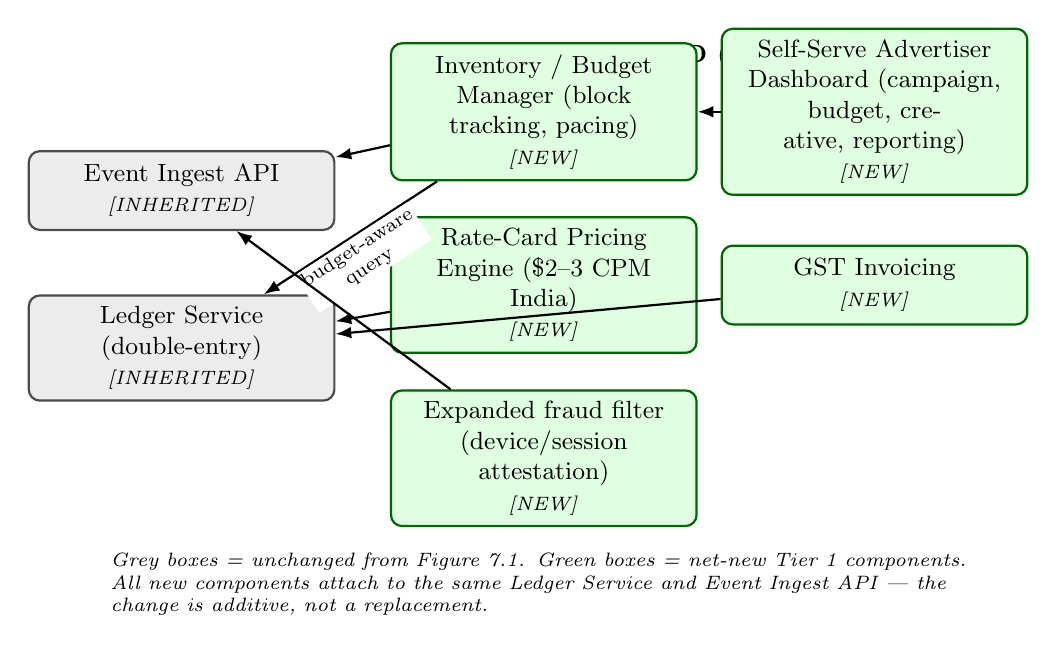
\begin{tikzpicture}[
    font=\small,
    inherited/.style={draw, thick, fill=gray!15, draw=gray!60!black, rounded corners, align=center, inner sep=4pt, text width=3.6cm, minimum height=1cm},
    newblock/.style={draw, thick, fill=green!12, draw=green!40!black, rounded corners, align=center, inner sep=4pt, text width=3.6cm, minimum height=1cm},
    arrlabel/.style={font=\scriptsize, align=center, fill=white, inner sep=1pt}
]

\node[font=\small\bfseries] (title) at (6.5,5.3) {Tier 1 --- BACKEND (rate-card serving)};

% Inherited boxes (greyed, from Figure 7.1)
\node[inherited] (ingest) at (0,3.6) {Event Ingest API\\\scriptsize\textit{[INHERITED]}};
\node[inherited] (ledger) at (0,1.6) {Ledger Service\\(double-entry)\\\scriptsize\textit{[INHERITED]}};

% New boxes (highlighted)
\node[newblock] (inventory) at (4.6,4.6) {Inventory / Budget\\Manager (block\\tracking, pacing)\\\scriptsize\textit{[NEW]}};
\node[newblock] (advdash) at (8.8,4.6) {Self-Serve Advertiser\\Dashboard (campaign,\\budget, creative, reporting)\\\scriptsize\textit{[NEW]}};
\node[newblock] (pricing) at (4.6,2.4) {Rate-Card Pricing\\Engine (\$2--3 CPM\\India)\\\scriptsize\textit{[NEW]}};
\node[newblock] (gst) at (8.8,2.4) {GST Invoicing\\\scriptsize\textit{[NEW]}};
\node[newblock] (fraud) at (4.6,0.2) {Expanded fraud filter\\(device/session\\attestation)\\\scriptsize\textit{[NEW]}};

% Connections: new boxes attach to inherited Ledger + Ingest
\draw[-{Latex[length=2mm]}, thick] (inventory) -- (ledger) node[midway, arrlabel, below, sloped] {budget-aware\\query};
\draw[-{Latex[length=2mm]}, thick] (advdash) -- (inventory);
\draw[-{Latex[length=2mm]}, thick] (pricing) -- (ledger);
\draw[-{Latex[length=2mm]}, thick] (gst) -- (ledger);
\draw[-{Latex[length=2mm]}, thick] (fraud) -- (ingest);
\draw[-{Latex[length=2mm]}, thick] (inventory) -- (ingest);

\node[font=\scriptsize\itshape, align=left, text width=11cm] at (4.6,-1.4) {Grey boxes = unchanged from Figure 7.1. Green boxes = net-new Tier 1 components. All new components attach to the same Ledger Service and Event Ingest API --- the change is additive, not a replacement.};

\end{tikzpicture}
\caption{Tier 1 component diagram: rate-card serving components (green, new) attach to the unchanged Ledger Service and Event Ingest API (grey, inherited from Figure~\ref{fig:v1-architecture}), demonstrating that Tier 1 bolts on without a rewrite.}
\label{fig:tier1-component}
\end{figure}

\subsection{Figure 7.4 --- Tier 2 future-state data-flow diagram}

\begin{figure}[htbp]
\centering
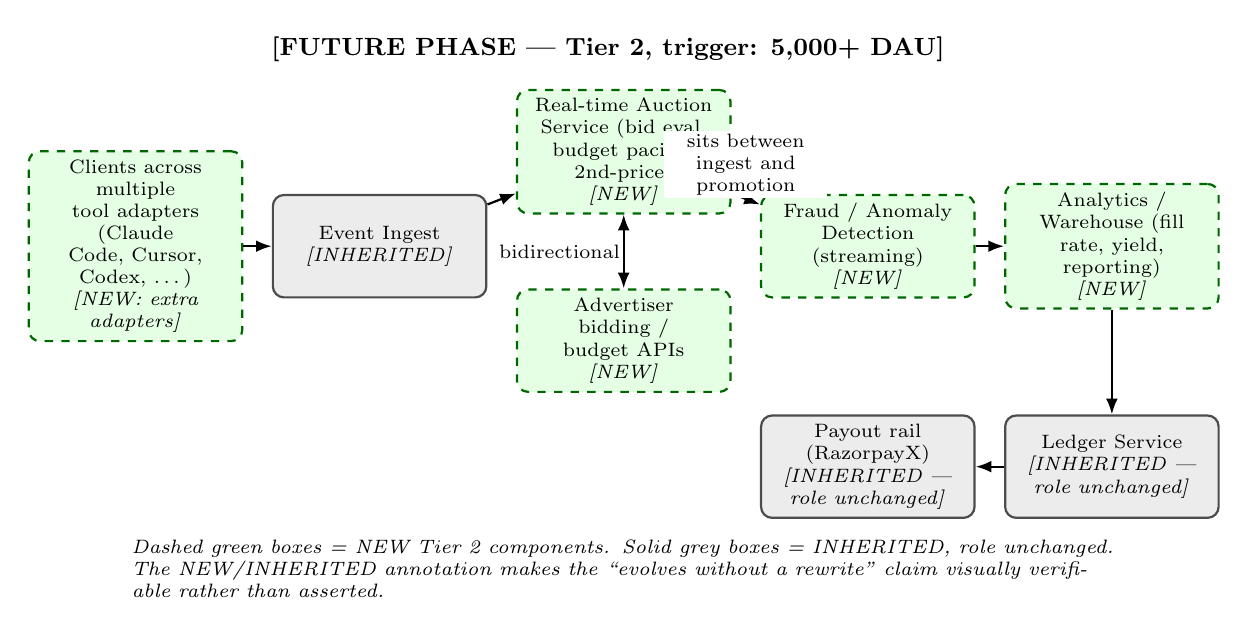
\begin{tikzpicture}[
    font=\scriptsize,
    inherited/.style={draw, thick, fill=gray!15, draw=gray!60!black, rounded corners, align=center, inner sep=3pt, text width=2.5cm, minimum height=1.3cm},
    newblock/.style={draw, thick, dashed, fill=green!10, draw=green!40!black, rounded corners, align=center, inner sep=3pt, text width=2.5cm, minimum height=1.3cm},
    arrlabel/.style={font=\scriptsize, align=center, fill=white, inner sep=1pt}
]

\node[font=\small\bfseries] (futuretag) at (6.0,4.0) {[FUTURE PHASE --- Tier 2, trigger: 5{,}000+ DAU]};

\node[newblock] (clients) at (0,1.5) {Clients across multiple\\tool adapters (Claude\\Code, Cursor, Codex, \ldots)\\\scriptsize\textit{[NEW: extra adapters]}};
\node[inherited] (ingest) at (3.1,1.5) {Event Ingest\\\scriptsize\textit{[INHERITED]}};
\node[newblock] (auction) at (6.2,2.7) {Real-time Auction\\Service (bid eval,\\budget pacing,\\2nd-price)\\\scriptsize\textit{[NEW]}};
\node[newblock] (bidapi) at (6.2,0.3) {Advertiser bidding /\\budget APIs\\\scriptsize\textit{[NEW]}};
\node[newblock] (fraud) at (9.3,1.5) {Fraud / Anomaly\\Detection\\(streaming)\\\scriptsize\textit{[NEW]}};
\node[newblock] (analytics) at (12.4,1.5) {Analytics /\\Warehouse (fill\\rate, yield, reporting)\\\scriptsize\textit{[NEW]}};
\node[inherited] (ledger) at (12.4,-1.3) {Ledger Service\\\scriptsize\textit{[INHERITED ---}\\\scriptsize\textit{role unchanged]}};
\node[inherited] (payout) at (9.3,-1.3) {Payout rail\\(RazorpayX)\\\scriptsize\textit{[INHERITED ---}\\\scriptsize\textit{role unchanged]}};

\draw[-{Latex[length=2mm]}, thick] (clients) -- (ingest);
\draw[-{Latex[length=2mm]}, thick] (ingest) -- (auction);
\draw[{Latex[length=2mm]}-{Latex[length=2mm]}, thick] (auction) -- (bidapi) node[midway, arrlabel, left] {bidirectional};
\draw[-{Latex[length=2mm]}, thick] (auction) -- (fraud) node[midway, arrlabel, above, text width=2.0cm] {sits between\\ingest and\\promotion};
\draw[-{Latex[length=2mm]}, thick] (fraud) -- (analytics);
\draw[-{Latex[length=2mm]}, thick] (analytics) -- (ledger);
\draw[-{Latex[length=2mm]}, thick] (ledger) -- (payout);

\node[font=\scriptsize\itshape, align=left, text width=12.5cm] at (6.2,-2.6) {Dashed green boxes = NEW Tier 2 components. Solid grey boxes = INHERITED, role unchanged. The NEW/INHERITED annotation makes the ``evolves without a rewrite'' claim visually verifiable rather than asserted.};

\end{tikzpicture}
\caption{Tier 2 future-state data-flow diagram [FUTURE PHASE]: real-time auction, streaming fraud detection, and an analytics warehouse are new peers sitting in front of the unchanged Ledger Service and payout rail.}
\label{fig:tier2-dataflow}
\end{figure}

\section{The honest read for the technical section}
\label{sec:honest-read}

The v1 architecture in \texttt{00-MVP-spec.md} is already correctly scoped for a solo founder, and the two external comps closest to this space --- Carbon Ads and EthicalAds --- validate it rather than challenge it. The temptation to resist is not under-building Tier 0; it is over-building toward Tier 2 too early, in engineering effort or in how the vision is presented. Every Tier 2 component (auction, fraud ML, analytics warehouse) is copyable technology once there is a reason to build it. The genuinely defensible technical claim is narrower and stronger: the \textbf{ledger and payout discipline --- double-entry, raw/billable separation, payable-not-wallet design, verified-webhook reconciliation --- built correctly at v1 is what lets Tier 1 and Tier 2 bolt on without a rewrite.} That discipline costs almost nothing extra now, and retrofitting it onto a live money system with real advertisers and real developer balances would be far more expensive and risky. That is the architecture's real moat --- not the spinner overlay, which was cloned across the category in 24 hours.

\chapter{Go-To-Market Strategy}
\label{chap:gtm}

\section{GTM Thesis}
\label{sec:gtm-overview}

The bottleneck for Devorix is demand, not supply (MASTER-PLAN \S4). Developers are not asking for this product; advertisers, meanwhile, have shockingly few high-trust placements for the agentic-coding moment. Devorix therefore seeds the \textbf{paying side first} -- cold advertiser outreach on Days 1--3 -- before building the developer-facing supply side on Days 3--10. This is a demand-led sequencing that matches documented best practice for B2B-leaning two-sided marketplaces, not a contrarian bet: demand-led seeding is the standard pattern where buyer economics justify joining a channel with thin existing supply \textbf{(Verified fact, marketplace cold-start literature)} \cite{internetmango_coldstart}.

The India-first, Ring-1-first plan is structurally an \emph{atomic network} strategy -- one dense niche conquered before broad expansion -- a recognized pattern from Andrew Chen's \textit{The Cold Start Problem}, not merely a founder preference \textbf{(Medium confidence -- framework applied to Devorix, not a quote about Devorix)} \cite{chen_coldstart_2021}.

\section{What the Comparable Launches Actually Prove}
\label{sec:gtm-comps}

These named comps are used here to temper and support specific claims, not to decorate the plan with borrowed credibility.

\begin{table}[htbp]
\centering
\caption{Comparable launch evidence and its limits}
\label{tab:gtm-comps}
\begin{tabular}{@{}p{2.0cm}p{4.6cm}p{4.6cm}p{1.6cm}@{}}
\toprule
\textbf{Comp} & \textbf{What it proves} & \textbf{What it does NOT prove for Devorix} & \textbf{Confidence} \\
\midrule
PostHog & A near-zero-budget HN+Twitter combo by a tiny team can reach real scale inbound-only: HN launch 4 weeks into building, \textasciitilde300 deployments in days, 1{,}000 users in \textasciitilde4 months, \$1M ARR by Oct 2020, \textasciitilde\$2{,}000 Twitter spend, no sales team. & That this works for an ad/rev-share product -- PostHog is a product developers actively wanted; Devorix monetizes a moment nobody asked to monetize. & Verified fact \\
Supabase & Product framing/timing can matter more than launch-day orchestration: HN launch posted by a third-party user, among the most-upvoted dev-tool launches ever (2nd to Stripe), with YC used as a credibility lever. & That Devorix's category gets the same organic pull -- this category's HN reception has been weak (see Kickbacks below). & Verified fact \\
T3 Chat / Theo Browne & Owned-audience-led growth converts faster than cold discovery: 60K+ users in months, 7-figure ARR on a pre-existing creator audience. & Not replicable -- the solo Devorix founder has no dev-influencer audience. & Verified fact \\
Permit.io & A sub-\$1{,}000 multi-channel launch push is in-budget for a \textasciitilde₹1-lakh (\textasciitilde\$1{,}150) constraint: \#1 Product of the Day on an \$800 total budget (Twitter Spaces micro-influencer + Instagram + YouTube). & That a Product Hunt ranking converts to durable installs or advertisers. & Verified fact \\
HN vs.\ PH head-to-head & HN converts visitors to installs far better than PH for dev tools, even when PH delivers more raw votes: same tool, HN \#2 front page (107 pts, 100+ installs) vs.\ PH \#14 (193 votes, \textasciitilde30 installs). & --- & Verified fact \\
Kickbacks (in-category) & In this exact category, Twitter/X -- not HN -- is the proven viral channel: Show HN got 2 points/0 comments, but the launch tweet hit 5.5M views in 24h. Single most important GTM data point for Devorix. & That virality converts to revenue -- it has not, for anyone in this category yet. & Verified fact \\
\bottomrule
\end{tabular}
\end{table}

\textbf{The hackathon-channel honesty flag (load-bearing).} No hard-numbers case study was found of any company whose \emph{primary} acquisition channel was hackathon sponsorship. Hackathon sponsorship is therefore labeled an \textbf{untested tactic} in this plan -- a plausible Month-2+ brand/awareness lever, not a proven Day 1--14 acquisition channel. The typical hackathon cold-sponsor conversion rate (\textasciitilde50 cold emails per sponsor closed -- \textbf{Industry estimate}) is structurally close to Devorix's own 12--15 pitches-per-yes assumption (Section~\ref{sec:gtm-launch-additions}), which suggests the advertiser-conversion assumption is realistic by category standards -- it says nothing, however, about hackathons as a \emph{user}-acquisition funnel.

\section{Concrete Additions to the Launch Motion}
\label{sec:gtm-launch-additions}

Building on the 14-day sprint structure (MASTER-PLAN \S8.2), three concrete additions sharpen the Days 10--14 launch motion:

\begin{enumerate}
  \item \textbf{Weight the launch tweet at least as heavily as the HN/PH submission.} This diverges from the general dev-tool pattern, where HN usually wins, because this specific category has already proven that Twitter is where it goes viral (the Kickbacks precedent, Section~\ref{sec:gtm-comps}).
  \item \textbf{Budget a tight \textasciitilde\$500--800 (\textasciitilde₹45,000--75,000) micro-influencer plus organic PH/HN push at launch}, mirroring Permit.io -- feasible only if scoped to one micro-influencer plus organic reach, not a paid campaign.
  \item \textbf{Make the client repository public.} This is a prerequisite for the GitHub Trending compounding effect: Trending ranks by star \emph{velocity}, so a small HN/Twitter spike can land a young repository on Trending for \textasciitilde48 hours \textbf{(Verified fact on the mechanism)}. \textit{(Medium confidence -- no named company with hard ``Trending $\rightarrow$ N installs'' numbers was found, so this is treated as a free secondary effect, not a planned channel.)} This also doubles as the trust/verification move described in Section~\ref{sec:self-critique} of Chapter~\ref{chap:business-strategy}.
\end{enumerate}

\section{Channel-by-Channel Honest Assessment}
\label{sec:gtm-channels}

\begin{table}[htbp]
\centering
\caption{Channel-by-channel honest assessment}
\label{tab:gtm-channel-assessment}
\begin{tabular}{@{}p{3.4cm}p{5.6cm}p{5.0cm}@{}}
\toprule
\textbf{Channel} & \textbf{Honest read} & \textbf{Role in plan} \\
\midrule
Hacker News / Show HN & High variance, out of our control; category precedent weak (Kickbacks: 2 points). & One-shot card, played only with a real payout/renewal story -- not the launch mechanism. \\
Product Hunt & Tool-collector audience, weak durable installs; good for backlinks/visibility. & Visibility, not retention. \\
Launch tweet / X & The proven in-category viral channel. & Primary launch-day lever. \\
GitHub (README / topic placement in Claude Code ecosystem repos) & Highest-leverage low-cost channel for this audience (27M India GitHub developers); earned, compounding, slow. & Core organic engine. \\
Hackathons / SIH / college fests & Untested as primary acquisition; conversion to active weekly user unproven, likely low. & Brand/awareness + ambassador recruiting, Month 2+. \\
Campus ambassadors & Cheapest real distribution (commission-only, paid via Devorix's own UPI rail -- eating its own dogfood). & Month 9--12 scale lever; hard ``don't oversell earnings'' rule required. \\
Cloud-provider India DevRel (AWS/GCP/Azure) & Plausible co-marketing, but not for a 2-week-old, zero-case-study product. & Month 12+ conversation only. \\
Enterprise (Infosys/TCS/Wipro) & Procurement cycles (3--6+ months) would burn the runway before revenue. & Deferred; cloud DevRel is the only ``enterprise-adjacent'' motion before Month 9. \\
\bottomrule
\end{tabular}
\end{table}

\section{Target List and Outreach Motion}
\label{sec:gtm-target-list}

The advertiser target list is organized into three concentric rings (MASTER-PLAN \S6.1), prioritized by how much persuasion each ring needs:

\begin{itemize}
  \item \textbf{Ring 1 -- AI-infra/dev-tool sellers to AI-building developers} (vector databases, observability, agent frameworks, scraping/data APIs such as Firecrawl, MCP tooling). Highest-probability first movers: both Kickbacks and IdleAds independently picked Firecrawl as their house placeholder, even as a fake placement -- they already believe this audience exists. Tactical targets: Razorpay DevTools, Sentry, PostHog, Hasura, DhiWise, Appsmith, Pabbly, 100ms, Supabase India, plus recently funded Indian startups filtered by India + SaaS + Seed/Series A + last 6 months.
  \item \textbf{Ring 2 -- India dev-economy sellers}: cloud/hosting resellers, EdTech/upskilling bootcamps (Scaler, Coding Ninjas, iNeuron, Newton School, Masai School), dev job boards, API/SaaS vendors with Indian GTM budgets. Budget and precedent exist -- they already buy Reddit and newsletter slots -- but they need more education on why this specific channel works.
  \item \textbf{Ring 3 -- Global dev-tool brands.} Explicit Phase 2 only, not a Month-1 target.
\end{itemize}

With zero warm advertiser intros confirmed at sprint start (MASTER-PLAN \S6.3), the sprint plan targets a list of 25--30 companies (not 20) and pitches 12--15 of them (not 5--10), to keep a realistic shot at the same close-rate bar used in earlier planning. The bar remains simple: \textbf{1 verbal yes = go; zero = stop and rethink.} Ring 1 is pitched first in every cohort, since it needs the least convincing.

\section{Roadmap Linkage}

The phase-by-phase channel sequencing summarized in Table~\ref{tab:gtm-channel-assessment} maps directly onto the 24-month roadmap phases described in Chapter~\ref{chap:roadmap}; channels are not deployed simultaneously but are unlocked as each phase's go/no-go gate clears.

\chapter{Financial Model: 12--24 Month Extension}
\label{ch:financial-model}

\section{Source map: every number traceable}

Three workbooks exist and disagree by design --- they are successive realism passes, not three live scenarios.

\begin{table}[htbp]
\centering
\caption{Source workbooks and their status}
\label{tab:source-workbooks}
\small
\begin{tabular}{p{3.4cm}p{5.6cm}p{4.0cm}}
\toprule
\textbf{Workbook} & \textbf{What it models} & \textbf{Status} \\
\midrule
\texttt{devorix-financial-\allowbreak model.xlsx} & Original aggressive ramp (500\(\to\)100,000 devs/12mo, fill 2\%\(\to\)55\%, \$2 eCPM) & \textbf{Superseded.} Stale \textrm{\textrupee}86 FX, CPM-only model that MASTER-PLAN \S 5 overrides. Kept only for the steady-state sensitivity table (Section~\ref{sec:unit-economics}). \\
\texttt{devorix-financial-\allowbreak model-REALISTIC.xlsx} & Grounded 4-month plan: \(\leq\) 500 installs, flat sponsorship deals, \textrm{\textrupee}94.5 FX & \textbf{Base case for Months 1--4.} Matches MASTER-PLAN \S 8.3 to the rupee. \\
\texttt{devorix-financial-\allowbreak model-v3-TIMEBASED.xlsx} & Same plan on a time-based (hours-coding \(\times\) \%-wait) impression count, plus a Global/Blended scenario & Used for impression mechanics, global sensitivity, and implied-eCPM cross-check. \\
\bottomrule
\end{tabular}
\end{table}

\textbf{Months 1--4 are not modeled here --- they are locked, audited inputs} that agree across MASTER-PLAN \S 8.3 and both current workbooks to the rupee \cite{masterplan_2026}.

\section{The honest stage framing}

Pre-launch, pre-revenue, 0 advertisers, 0 installs, solo founder, \textrm{\textrupee}1 lakh budget. \textbf{Founder salary is modeled at \textrm{\textrupee}0 (sweat equity)} --- these are not fully-loaded costs and exclude founder opportunity cost entirely; investors should read margins with that in mind. Everything past Month 4 is gated on MASTER-PLAN \S 8.3's go/no-go test (\(\geq\) 2 advertisers paid \emph{and} renewed, week-4 retention holds, founder still wants to run it). The 12--24 month curves are \textbf{planning scaffolding, not a funded forecast}.

\section{Months 1--4: locked base case}
\label{sec:months-1-4}

\begin{table}[htbp]
\centering
\caption{Months 1--4 locked base case (audited, not modeled)}
\label{tab:months-1-4}
\small
\begin{tabular}{lrrrrl}
\toprule
\textbf{Metric} & \textbf{M1} & \textbf{M2} & \textbf{M3} & \textbf{M4} & \textbf{Source / Label} \\
\midrule
Installs (cumulative) & 100 & 250 & 400 & 500 & \textit{Verified (locked input)} \\
Active devs (WAU 40\%) & 40 & 100 & 160 & 200 & Same \\
Advertisers (flat deals) & 1 & 2 & 2 & 3 & Same \\
Revenue (\textrm{\textrupee}) & 15,000 & 30,000 & 30,000 & 45,000 & Same \\
Dev payout pool (\textrm{\textrupee}, 50\%) & 7,500 & 15,000 & 15,000 & 22,500 & Same \\
Fixed costs (\textrm{\textrupee}) & 5,060 & 5,120 & 5,120 & 5,180 & infra \textrm{\textrupee}3,000 + misc \textrm{\textrupee}2,000 + payout txn \\
Net profit (\textrm{\textrupee}) & 2,440 & 9,880 & 9,880 & 17,320 & Same \\
\textbf{Cumulative net (\textrm{\textrupee})} & 2,440 & 12,320 & 22,200 & \textbf{39,520} & Matches MASTER-PLAN \S 8.3's ``\textasciitilde 39,500'' \\
Implied eCPM (\textrm{\textrupee}/1,000 views, v3) & 19.7 & 15.8 & 9.9 & 11.8 & Flat-fee underprices impressions as audience grows \\
\bottomrule
\end{tabular}
\end{table}

\begin{figure}[htbp]
\centering
\begin{tikzpicture}[
  every node/.style={font=\small},
  box/.style={draw, rectangle, minimum width=3.0cm, minimum height=1.0cm, align=center},
  neg/.style={draw, rectangle, minimum width=3.0cm, minimum height=1.0cm, align=center, fill=red!15},
  posbox/.style={draw, rectangle, minimum width=3.0cm, minimum height=1.0cm, align=center, fill=green!15}
]
\node[box, fill=blue!15] (rev) at (0,0) {Revenue\\ \textrm{\textrupee}45,000};
\node[neg, right=1.2cm of rev] (payout) {Dev payout\\ \(-\)\textrm{\textrupee}22,500};
\node[neg, right=1.2cm of payout] (fixed) {Fixed costs\\ \(-\)\textrm{\textrupee}5,180};
\node[posbox, right=1.2cm of fixed] (net) {Net\\ \textrm{\textrupee}17,320};

\draw[-{Stealth[length=3mm]}, thick] (rev) -- (payout);
\draw[-{Stealth[length=3mm]}, thick] (payout) -- (fixed);
\draw[-{Stealth[length=3mm]}, thick] (fixed) -- (net);

\node[font=\scriptsize\itshape, align=center] at (0,-1.3) {founder salary \textrm{\textrupee}0\\(sweat equity)};
\draw[-{Stealth[length=2mm]}, dashed] (0,-1.0) -- (rev.south);
\end{tikzpicture}
\caption{Tier-0 unit-economics waterfall, Month 4 (locked base case).}
\label{fig:waterfall-m4}
\end{figure}

\begin{figure}[htbp]
\centering
\begin{tikzpicture}
\begin{axis}[
  width=11cm, height=6.5cm,
  xlabel={Month}, ylabel={Implied eCPM (\textrm{\textrupee}/1,000 views)},
  xtick={1,2,3,4}, xticklabels={M1,M2,M3,M4},
  ymin=0, ymax=24,
  legend pos=north east,
  grid=major, grid style={dashed, gray!30},
]
\addplot[mark=*, thick, blue] coordinates {(1,19.7) (2,15.8) (3,9.9) (4,11.8)};
\legend{Implied eCPM, Tier 0}
\end{axis}
\node[font=\scriptsize\itshape, align=left] at (6.0,0.3) {Flat-fee underprices the audience as it grows --- the reason the};
\node[font=\scriptsize\itshape, align=left] at (6.05,-0.15) {pricing ladder moves to CPM at Tier 1.};
\end{tikzpicture}
\caption{Implied-eCPM decay under Tier-0 flat-fee pricing as the active-developer base grows.}
\label{fig:ecpm-decay}
\end{figure}

\section{Months 5--24: three scenarios}
\label{sec:scenarios}

No workbook models past Month 4. The extension below is new planner work --- Tier-0 flat-fee economics held until MASTER-PLAN \S 5.1's Tier-1 trigger (5--10 advertisers signed), then per-advertiser revenue converts to the Tier-1 rate card (\$2--3 CPM India, dev share \(\approx\) \$1--1.5/block \(\approx\) \textrm{\textrupee}94--141 at the locked \textrm{\textrupee}94 FX). The install curve is a planner-constructed S-curve consistent with the \emph{observed} M1--M4 growth rate, not a researched adoption curve. All figures past Month 4 are \textbf{\textit{[Internal assumption --- planner extrapolation]}}.

\begin{table}[htbp]
\centering
\caption{Worst-case scenario, M4--M24}
\label{tab:scenario-worst}
\small
\begin{tabular}{lrrrrrr}
\toprule
& \textbf{M4 (locked)} & \textbf{M6} & \textbf{M9} & \textbf{M12} & \textbf{M18} & \textbf{M24} \\
\midrule
Installs (cum.) & 500 & 550 & 600 & 650 & \textasciitilde 700 & \textasciitilde 700 \\
Advertisers & 3 & 2 (no renewal) & 1 & 1 & 1 & 1 \\
Revenue (\textrm{\textrupee}/mo) & 45,000 & 30,000 & 15,000 & 15,000 & 15,000 & 15,000 \\
Tier & 0 & 0 & 0 & 0 & 0 & 0 \\
Net profit (\textrm{\textrupee}/mo) & 17,320 & \textasciitilde 9,800 & \textasciitilde 5,000 & \textasciitilde 5,000 & \textasciitilde 5,000 & \textasciitilde 5,000 \\
\bottomrule
\end{tabular}
\end{table}

\begin{table}[htbp]
\centering
\caption{Likely-case scenario, M4--M24}
\label{tab:scenario-likely}
\small
\begin{tabular}{lrrrrrr}
\toprule
& \textbf{M4 (locked)} & \textbf{M6} & \textbf{M9} & \textbf{M12} & \textbf{M18} & \textbf{M24} \\
\midrule
Installs (cum.) & 500 & 900 & 1,600 & 2,800 & \textasciitilde 5,500 & \textasciitilde 9,000 \\
Advertisers & 3 & 4 & 6 (Tier 1 activates) & 8 & 8--10 & 10 \\
Revenue (\textrm{\textrupee}/mo) & 45,000 & 60,000 & \textasciitilde 95,000 & \textasciitilde 165,000 & \textasciitilde 150,000--250,000 & \textasciitilde 150,000--300,000 \\
Net profit (\textrm{\textrupee}/mo) & 17,320 & \textasciitilde 28,000 & \textasciitilde 42,000 & \textasciitilde 78,000 & \textasciitilde 150,000 & \textasciitilde 280,000 \\
Cumulative net (\textrm{\textrupee}) & 39,520 & \textasciitilde 110,000 & \textasciitilde 280,000 & \textasciitilde 650,000 & \textasciitilde 1,500,000 & \textasciitilde 3,200,000 \\
\bottomrule
\end{tabular}
\end{table}

\begin{table}[htbp]
\centering
\caption{Best-case scenario, M4--M24}
\label{tab:scenario-best}
\small
\begin{tabular}{lrrrrrr}
\toprule
& \textbf{M4 (locked)} & \textbf{M6} & \textbf{M9} & \textbf{M12} & \textbf{M18} & \textbf{M24} \\
\midrule
Installs (cum.) & 500 & 1,500 & 4,000 & 8,000 & \textasciitilde 16,000 & \textasciitilde 30,000 \\
Advertisers & 3 & 6 & 10 & 15 & 18 & 20+ \\
Revenue (\textrm{\textrupee}/mo) & 45,000 & 110,000 & \textasciitilde 300,000 & \textasciitilde 620,000 & \textasciitilde 850,000 & \textasciitilde 1,600,000 \\
Net profit (\textrm{\textrupee}/mo) & 17,320 & \textasciitilde 70,000 & \textasciitilde 210,000 & \textasciitilde 450,000 & \textasciitilde 850,000 & \textasciitilde 1,600,000 \\
Cumulative net (\textrm{\textrupee}) & 39,520 & \textasciitilde 230,000 & \textasciitilde 900,000 & \textasciitilde 2,500,000 & \textasciitilde 6,500,000 & \textasciitilde 14,000,000 \\
\bottomrule
\end{tabular}
\end{table}

\textbf{Reconciliation note on the two source models' M24 figures.} The TAM-research scenario table and the planner financial extension were built independently and converge closely for the \textbf{Likely} case (both land \textasciitilde \textrm{\textrupee}150k--300k/mo, \textasciitilde 5,000--9,000 installs at M24). They diverge on the \textbf{Best} case: the TAM research caps best-case M24 at \textasciitilde \textrm{\textrupee}500k--900k/mo (12,000--20,000 installs), while the planner extension runs to \textasciitilde \textrm{\textrupee}1.6M/mo (30,000 installs). We present the planner figures as the upper rail and the TAM-research figures as a more conservative best case, and treat the \emph{Likely} convergence as the load-bearing number. The Best-case divergence is two compounding layers of unverified assumption and should be read as a thought experiment, not diligence.

\begin{figure}[htbp]
\centering
\begin{tikzpicture}
\begin{axis}[
  width=12cm, height=7cm,
  xlabel={Month}, ylabel={Revenue (\textrm{\textrupee}/mo)},
  xtick={4,6,9,12,18,24},
  ymin=0, ymax=1700000,
  legend pos=north west,
  grid=major, grid style={dashed, gray!30},
  scaled y ticks=false,
  yticklabel style={/pgf/number format/.cd, fixed, fixed zerofill=false, 1000 sep={,}},
]
\addplot[mark=square*, thick, red!70!black] coordinates {(4,45000) (6,30000) (9,15000) (12,15000) (18,15000) (24,15000)};
\addplot[mark=*, thick, blue] coordinates {(4,45000) (6,60000) (9,95000) (12,165000) (18,200000) (24,280000)};
\addplot[mark=triangle*, thick, green!50!black] coordinates {(4,45000) (6,110000) (9,300000) (12,620000) (18,850000) (24,1600000)};
\draw[dashed, gray] (axis cs:9,0) -- (axis cs:9,1700000);
\node[font=\scriptsize, anchor=south west] at (axis cs:9,1620000) {Tier-1 activation (Likely, \textasciitilde M9)};
\legend{Worst, Likely, Best}
\end{axis}
\end{tikzpicture}
\caption{24-month revenue scenarios. Tier 2 (real-time auction, 5,000+ DAU threshold) is not reached in any scenario through M12.}
\label{fig:revenue-scenarios}
\end{figure}

\begin{figure}[htbp]
\centering
\begin{tikzpicture}
\begin{axis}[
  width=12cm, height=7cm,
  xlabel={Month}, ylabel={Cumulative net profit (\textrm{\textrupee})},
  xtick={4,12,24},
  ymin=0, ymax=14500000,
  legend pos=north west,
  grid=major, grid style={dashed, gray!30},
  scaled y ticks=false,
  yticklabel style={/pgf/number format/.cd, fixed, fixed zerofill=false, 1000 sep={,}},
]
\addplot[mark=square*, thick, red!70!black] coordinates {(4,39520) (12,99520) (24,159520)};
\addplot[mark=*, thick, blue] coordinates {(4,39520) (12,650000) (24,3200000)};
\addplot[mark=triangle*, thick, green!50!black] coordinates {(4,39520) (12,2500000) (24,14000000)};
\legend{Worst (flat \textasciitilde\textrm{\textrupee}5,000/mo accrual), Likely, Best}
\end{axis}
\node[font=\scriptsize\itshape, align=left] at (6.6,-0.4) {All post-M4 points: Internal assumption --- planner extrapolation.};
\end{tikzpicture}
\caption{Cumulative net profit by scenario, M4--M24.}
\label{fig:cumulative-net}
\end{figure}

\subsection*{Reading the scenarios}

\textbf{Worst case is not ``zero'' --- it is ``stuck at Tier 0 indefinitely,''} which is still cash-flow-positive against the \textasciitilde \textrm{\textrupee}5,000/mo cost base. This is precisely the ``stop and rethink'' branch MASTER-PLAN \S 8.3 defines: if \(\geq\) 2 advertisers don't renew, the plan says stop, not keep projecting. Shown for completeness, not as a target.

\textbf{Likely case} assumes the gate clears and at least one of the two structural bottlenecks (advertiser sales; retention past novelty) resolves favorably --- not both.

\textbf{Best case} requires both to resolve favorably \emph{and} requires IdleAds' 70\%/90\%-goal rev-share not to meaningfully erode Devorix's developer supply against the locked 50/50.

\textbf{The single most important caveat:} even the BEST case stays inside the Tier 0/Tier 1 hybrid pricing regime through Month 12 --- 8,000 installs is still well short of the 5,000+ DAU threshold for Tier 2 (real-time auction). Tier 2 is realistically an 18--24 month conversation under every scenario. Two real-world facts puncture any naive continuation of these curves: (1) IdleAds already offers a 70\% dev rev-share versus the locked 50\% --- dev-supply competition is a real risk to the install curve at this horizon, not a footnote (flagged for monitoring, \emph{not} a reopening of the locked 50/50 decision); (2) the category is 2.5 weeks old with zero proven advertiser retention anywhere --- a 24-month projection here is closer to a thought experiment than a forecast.

\section{Unit economics}
\label{sec:unit-economics}

\begin{table}[htbp]
\centering
\caption{Unit economics}
\label{tab:unit-economics}
\small
\begin{tabular}{p{4.0cm}p{3.4cm}p{2.6cm}p{3.0cm}}
\toprule
\textbf{Metric} & \textbf{Value} & \textbf{Source} & \textbf{Label / Note} \\
\midrule
Revenue / active dev / month (Tier 0, M4) & \textrm{\textrupee}225 gross (\textrm{\textrupee}45,000 \(\div\) 200) & REALISTIC \texttt{Plan\_4mo\_FlatDeals} & Dev share = \textrm{\textrupee}112.50 \\
Dev payout / active dev / month (Tier 0, M1--M4) & \textrm{\textrupee}93.75--\textrm{\textrupee}187.50 & Same & \textbf{Non-monotonic} --- drops M1\(\to\)M3 (\textrm{\textrupee}187.50\(\to\)\textrm{\textrupee}93.75) as installs outpace flat-fee advertiser revenue, recovers M4 \\
Revenue / advertiser / month (Tier 0) & \textrm{\textrupee}15,000 flat & MASTER-PLAN \S 5.1--5.2; all 3 workbooks & \textbf{Locked} --- the number to quote in pitches, not CPM-derived \\
Revenue / advertiser / month (Tier 1) & \$2--3 CPM-equiv.\ India; depends on audience at activation & MASTER-PLAN \S 5.4 & \textit{[Internal assumption -- revisit once Tier 1 has real fill data]} (founder's tag) \\
Contribution margin per \textrm{\textrupee} revenue & 50\% (= dev rev share), before fixed costs & Decision \#11; all workbooks & Payout txn cost (\textrm{\textrupee}3--4/txn, RazorpayX) \(\approx\) \textrm{\textrupee}180/mo at M4 = 0.4\% of revenue, rounds to \textasciitilde 0 \\
Fixed costs / month (Tier 0 era) & \textasciitilde \textrm{\textrupee}5,000--5,200 (infra \textrm{\textrupee}3,000 + misc \textrm{\textrupee}2,000 + payout fees) & REALISTIC & Founder salary = \textrm{\textrupee}0 (sweat equity) --- flag to investors: not fully-loaded \\
Tier 0 \(\to\) 1 step-change & From a share of flat \textrm{\textrupee}15,000 (no per-impression accounting) to \$1--1.5/block (\textrm{\textrupee}94--141) priced per filled impression & MASTER-PLAN \S 5.1, \S 5.4 & A pricing-\emph{model} change, not just volume; requires the block-serving engine to exist (\texttt{00-MVP-spec.md} \S 4, not yet built) \\
Steady-state per-dev ceiling (sanity check, NOT the plan) & \textrm{\textrupee}151.36/dev/month at \$2 eCPM, 100\% fill & \texttt{devorix-financial-model.xlsx} \texttt{Scenarios} & \textbf{Superseded model} --- upper-bound only; 100\% fill unrealistic at any modeled horizon \\
Reality-check floor (why CPM-only fails at small scale) & 500 installs / 200 active / 15\% fill \(\to\) gross \textrm{\textrupee}4,990/mo, dev share \textrm{\textrupee}2,495/mo total (\(\approx\) \textrm{\textrupee}12.47/active dev/mo) & REALISTIC \texttt{Reality\_Check\_CPM} & The workbook's own justification for why Tier 0 must be flat-fee --- load-bearing for MASTER-PLAN \S 5's whole pricing architecture \\
\bottomrule
\end{tabular}
\end{table}

\textbf{Headline unit-economics read:} at Tier 0, each advertiser is a clean \textrm{\textrupee}15,000/mo at 50\% contribution margin, and the business is cash-positive from Month 1 because costs are \textasciitilde \textrm{\textrupee}5,000/mo. The non-monotonic per-dev payout is the clearest single signal that flat-fee pricing is a deliberate early-stage choice (sellable at small scale) that underprices the audience as it grows --- which is exactly why the ladder moves to CPM at Tier 1.

\section{Sensitivity: which assumptions move the model most}
\label{sec:sensitivity}

Ranked by modeled swing, drawn from the workbooks' own sensitivity sheets plus the M4--M24 extension.

\begin{table}[htbp]
\centering
\caption{Sensitivity ranking}
\label{tab:sensitivity}
\small
\begin{tabular}{cp{3.2cm}p{2.6cm}p{4.4cm}p{2.4cm}}
\toprule
\textbf{Rank} & \textbf{Assumption} & \textbf{Range tested} & \textbf{Effect on monthly platform margin} & \textbf{Source} \\
\midrule
1 & \textbf{Fill rate} (\% of impressions sold to a paying advertiser) & 5\% \(\to\) 100\% & At 200 active devs: \textrm{\textrupee}9,029 \(\to\) \textrm{\textrupee}180,576 gross/mo --- a \textbf{20\(\times\)} swing from this variable alone & v3 \texttt{Platform\_Scale} --- called ``THE constraint'' \\
2 & \textbf{Active-developer count} (install\(\to\)WAU funnel) & 50 \(\to\) 500 devs & At fixed 30\% fill: \textrm{\textrupee}27,086 \(\to\) \textrm{\textrupee}270,864 gross/mo --- a \textbf{10\(\times\)} swing & v3 \texttt{Platform\_Scale} --- compounds multiplicatively with rank 1 \\
3 & \textbf{Pricing-model choice} (flat vs.\ CPM) at same audience & Flat \textrm{\textrupee}15,000/advertiser vs.\ CPM & Same 3.8M views/mo: flat = \textrm{\textrupee}30,000 (eCPM \textrm{\textrupee}7.89) vs.\ CPM = \textrm{\textrupee}108,346 (eCPM \textrm{\textrupee}28.50) --- a \textbf{3.6\(\times\)} difference for identical usage & v3 \texttt{CPM\_vs\_FlatDeal} \\
4 & \textbf{eCPM level} (secondary) & \$0.8 \(\to\) \$5.0 & At 10,000 devs, full fill: \textrm{\textrupee}6.05L \(\to\) \textrm{\textrupee}37.84L/mo --- \textbf{6.25\(\times\)} & \texttt{devorix-financial-model.xlsx} \texttt{Scenarios} --- superseded \textrm{\textrupee}86 FX/CPM-only; directionally valid \\
5 & \textbf{Going global} (\% foreign users, secondary) & 0\% \(\to\) 20\% foreign & Same 200 active base: India-only \textrm{\textrupee}108,346/mo vs.\ blended \textrm{\textrupee}194,338/mo --- a \textbf{1.79\(\times\)} uplift & v3 \texttt{Global\_Blended} --- gated behind MASTER-PLAN \S 8.1's ``Global = Phase 2'' \\
\bottomrule
\end{tabular}
\end{table}

\begin{figure}[htbp]
\centering
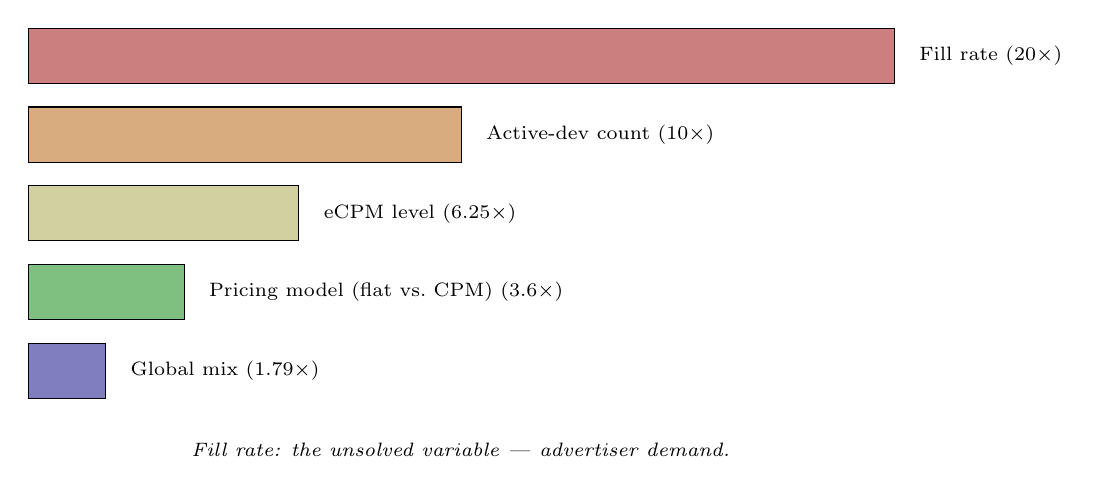
\begin{tikzpicture}[every node/.style={font=\small}]
\def\scl{0.55}
\foreach \rank/\lbl/\val/\col in {%
  1/{Fill rate}/20/red!60!black,%
  2/{Active-dev count}/10/orange!70!black,%
  3/{eCPM level}/6.25/yellow!60!black,%
  4/{Pricing model (flat vs.\ CPM)}/3.6/green!50!black,%
  5/{Global mix}/1.79/blue!50!black%
} {
  \pgfmathsetmacro{\ypos}{-(\rank-1)*1.0}
  \node[draw, fill=\col, fill opacity=0.5, draw opacity=1, minimum height=0.7cm, minimum width=\val*\scl cm, anchor=west] at (0,\ypos) {};
  \node[anchor=west, font=\scriptsize] at (\val*\scl+0.2,\ypos) {\lbl\ (\val\(\times\))};
}
\node[font=\scriptsize\itshape, align=left] at (5.5,-5.0) {Fill rate: the unsolved variable --- advertiser demand.};
\end{tikzpicture}
\caption{Sensitivity tornado: modeled swing in monthly platform margin by assumption.}
\label{fig:sensitivity-tornado}
\end{figure}

\textbf{Why this matters for the risk framing:} the top two levers --- fill rate and active-dev count --- are both downstream of the same root cause MASTER-PLAN names as the central risk: \textbf{advertiser demand, not developer supply, is the bottleneck}. Fill rate is literally ``can we find advertisers to buy inventory we already have.'' The model is far more sensitive to a variable nobody has solved yet (fill rate) than to a comparatively tractable one (install growth). The PRD's financial model should lead with this, not bury it. The CPM rate and 50/50 split are locked and not modeled as variables --- but for the risk section: IdleAds' 70\%/90\%-goal split is an advertiser-supply-indifferent lever a competitor can pull that Devorix has chosen not to. A competitive sensitivity worth flagging, not a reopening of the locked decision.

\section{Open numeric gaps for further research (financial)}

\begin{enumerate}
  \item Realistic \textbf{fill-rate trajectory} month-over-month once \(\geq\) 1 advertiser is signed --- rank \#1 sensitivity, currently a blue-cell assumption in every workbook (5\%\(\to\)100\% original, 15\% REALISTIC, 30\% v3) with no empirical basis. Highest-value number to replace with real data after the sprint.
  \item \textbf{Week-4 developer retention} --- a \S 8.3 go/no-go condition; no workbook models churn, only cumulative installs.
  \item \textbf{Ring 1 + Ring 2 total addressable ad budget} (the Tier-1/Tier-2 revenue ceiling) --- unsized anywhere.
  \item \textbf{India-specific dev-tool-marketer ad spend} --- all current comps (Carbon Ads, EthicalAds, Stack Overflow Ads) are US/global; Devorix is India-first.
\end{enumerate}

\bigskip
\noindent\textit{Near-term locked inputs (Months 1--4, Section~\ref{sec:months-1-4}) are audited and load-bearing for the funding ask. All 12--24 month figures (Section~\ref{sec:scenarios}, and rows 4--5 of Section~\ref{sec:sensitivity}) are labeled Internal assumption / vision-context and must not be presented to investors as derived from the workbooks --- only Months 1--4 are.}

\chapter{Risk Analysis}
\label{chap:risk-analysis}

\section{Consolidated Risk Register}
\label{sec:risk-register}

The register below consolidates risks surfaced across the original MASTER-PLAN risk discussion (\S10/\S11), the GTM research cluster, and the user-research cluster. Severity is rated on a four-point scale -- \textbf{Critical / High / Medium / Low} -- and status is rated as \textbf{Monitored} (watched at a defined trigger, no action required now) or \textbf{Needs-action} (a concrete near-term to-do exists).

\begin{longtable}{@{}p{0.6cm}p{3.6cm}p{4.6cm}p{1.5cm}p{1.7cm}p{3.6cm}@{}}
\caption{Consolidated risk register (R1--R12)}
\label{tab:risk-register} \\
\toprule
\textbf{\#} & \textbf{Risk} & \textbf{Detail \& source} & \textbf{Severity} & \textbf{Status} & \textbf{Trigger / action} \\
\midrule
\endfirsthead
\multicolumn{6}{c}{\tablename\ \thetable{} -- continued from previous page} \\
\toprule
\textbf{\#} & \textbf{Risk} & \textbf{Detail \& source} & \textbf{Severity} & \textbf{Status} & \textbf{Trigger / action} \\
\midrule
\endhead
R1 & Demand-side: zero verified paying advertisers exist anywhere in the category & Single biggest risk to the whole thesis; nobody has proven a brand will pay for a wait-state placement (MASTER-PLAN \S3, \S11). & Critical & Needs-action & The 14-day sprint exists to test this. Action: 1 verbal yes = go; 0 = stop. \\
R2 & IdleAds rev-share undercut (70\%, 90\% stated goal vs.\ Devorix's locked 50/50) & Direct competitor offers materially better dev economics; threatens Tier-1 dev-supply quality (MASTER-PLAN \S10/\S11). \textbf{The locked 50/50 split is final -- this is a risk to monitor, not a reason to revisit it.} & High & Monitored & Trigger: if Month 9--12 dev signups stall specifically on rev-share comparison (not novelty fatigue), revisit pricing levers other than the split itself (trust, UPI reliability, UX). \\
R3 & Anthropic anti-ads brand campaign -- ``Ads are coming to AI. But not to Claude'' (Super Bowl, Feb 2026) & Anthropic has publicly and prominently positioned Claude as the explicitly ad-free AI. Devorix puts a sponsor line on Claude Code's surface -- a direct narrative collision with the platform owner's public brand stance, sharpening the platform-sentiment/ToS-perception risk beyond the purely technical ToS line. & High & Needs-action & Action: tighten the ``we are a non-patching, opt-in developer revenue-share tool, not an ad injected into Claude's product'' framing; keep the compliance appendix (Section~\ref{sec:risk-compliance}) explicit; monitor Anthropic policy statements. Engineering discipline alone does not cover the brand-perception dimension. \\
R4 & IdleAds positioning collision -- already claims the same trust positioning Devorix plans to use & The trust/``clean, honest'' angle Devorix intended as a differentiator is already asserted by a competitor, weakening the best near-term moat candidate (Chapter~\ref{chap:business-strategy}, Section~\ref{sec:moats}). & Medium-High & Needs-action & Action: make trust verifiable, not asserted -- open-source the client or publish a data-flow doc (Chapter~\ref{chap:business-strategy}, Section~\ref{sec:self-critique}). Verifiability is the part IdleAds has not done, and is harder to copy than a claim. \\
R5 & Platform-policy / ToS (technical) & Anthropic's January 2026 enforcement blocked OAuth-token-reusing third-party clients; the CLI binary plus official API keys remain explicitly allowed. Devorix's non-patching, token-untouching client sits on the safe side of this line -- conditional on engineering discipline being maintained (MASTER-PLAN \S10/\S11). & Medium & Monitored & Trigger: any change in Anthropic's Consumer Terms; any drift toward patching. Maintain the ``we are not Kickbacks'' compliance appendix. \\
R6 & Regulatory -- RBI PPI rules actively in flux & RBI issued draft Master Directions revisiting PPI rules in April 2026. The accrue-then-payout ledger likely sits outside PPI scope, but the area is actively moving (MASTER-PLAN \S7.1/\S11). & Medium & Needs-action & Action: obtain CA/fintech-lawyer sign-off on ledger design before scaling past MVP, not after. \\
R7 & Trust environment -- category guilt-by-association & ``IDEsaster'' (30+ disclosed vulnerabilities across AI coding tools), plus a June 2026 Microsoft open-source supply-chain attack; developers are primed to distrust anything touching their dev environment. A scandal at Kickbacks or IdleAds could splash onto Devorix (MASTER-PLAN \S10/\S11). & Medium & Monitored & Trigger: any category-wide trust incident. Mitigation overlaps R4 (verifiable non-patching claim). \\
R8 & Solo-founder bandwidth & Plan assumes the founder runs sales, support, and product simultaneously through Month 4+; advertiser-relationship quality (the real differentiator) degrades if support load dominates (Chapter~\ref{chap:business-strategy}, Section~\ref{sec:self-critique}). & Medium & Needs-action & Action: add the Month-3 time-budget self-check gate described in Chapter~\ref{chap:business-strategy}. \\
R9 & Pricing power / panic-discount anchoring & At 1--3 advertisers, every deal is negotiated from need; the first deal can anchor all future deals low (Chapter~\ref{chap:business-strategy}, Section~\ref{sec:self-critique}). & Medium & Needs-action & Action: institute the ₹8,000/mo price floor rule before the first negotiation. \\
R10 & Compliance/tax timing (TDS/GST) & Section 194H TDS is effectively nil pre-₹1cr deductor turnover; GST is not required below ₹20L/yr; both re-verified (MASTER-PLAN \S7.1). Low risk now, attaches with scale. & Low & Monitored & Trigger: first deal requiring a GST invoice; turnover crossing the relevant thresholds. Collect PAN from advertisers regardless. \\
R11 & Rebrand (Async Returns $\rightarrow$ Devorix, 2026-06-28) untested & The name changed the day before this PRD work began; there has been no time to test resonance with developers or advertisers (Chapter~\ref{chap:business-strategy}, Section~\ref{sec:self-critique}). & Low & Monitored & Trigger: launch-cohort feedback. \\
R12 & Hackathon channel unproven as primary acquisition & No case study of hackathon-as-primary-channel was found (Chapter~\ref{chap:gtm}, Section~\ref{sec:gtm-comps}). & Low & Monitored & Action: budget as brand/awareness only; do not set a CAC target against it. \\
\bottomrule
\end{longtable}

\section{Narrative: The Top Risks}
\label{sec:risk-narrative}

\subsection{R1 --- Zero verified paying advertisers exist anywhere in the category (Critical, Needs-action)}

This is the single largest risk to the entire thesis, and it is a category-wide problem, not a Devorix-specific weakness. As of this writing, nobody -- not Devorix, not Kickbacks, not IdleAds -- has proven that a brand will pay for a wait-state placement at any price. Both Kickbacks and IdleAds independently used Firecrawl as a house placeholder advertiser, not a paying customer, which is itself the strongest signal in the space: AI-infra and dev-tool sellers are believed by everyone in this category to be the natural first buyer, yet nobody has closed one. The entire 14-day sprint (MASTER-PLAN \S8.2) exists specifically to test this risk directly, with a binary, pre-committed exit rule: one verbal yes from a real advertiser means continue; zero means stop and rethink before building anything further. No amount of product polish substitutes for this test.

\subsection{R2 --- IdleAds rev-share undercut: 70\%, 90\% stated goal, vs.\ Devorix's locked 50/50 (High, Monitored)}

IdleAds offers developers materially better headline economics than Devorix. This is a real, durable competitive gap, not a misunderstanding to be argued away. It is explicitly \emph{not} a reason to revisit the locked 50/50 split (MASTER-PLAN decision \#11, DECIDED FINAL) -- the split is final business-model architecture, and the right response is to compete on dimensions other than the split itself: India-native automated UPI payout reliability, verifiable non-patching trust, and advertiser placement quality. The monitoring trigger is specific and falsifiable: if developer signups stall in Month 9--12 \emph{specifically} because of rev-share comparison shopping -- not generic novelty fatigue -- that is the signal to revisit non-split pricing levers, not the percentage itself.

\subsection{R3 --- Anthropic's anti-ads brand campaign creates a narrative collision (High, Needs-action)}

Anthropic ran a prominent public campaign -- ``Ads are coming to AI. But not to Claude,'' timed to the Super Bowl in February 2026 -- explicitly positioning Claude as the ad-free AI assistant. Devorix's entire mechanic places a sponsor line on Claude Code's own surface. This is a genuine collision between Devorix's business model and the platform owner's public brand stance, and it is a sharper, more public-facing risk than the underlying technical ToS question (R5). Engineering discipline on the non-patching architecture does not, by itself, address this -- the risk lives at the level of brand perception and narrative framing, not code. The mitigating action is to consistently and explicitly frame Devorix as an opt-in developer revenue-share tool that the developer chooses to run, not an ad injected into Anthropic's product by Anthropic or without consent, and to keep monitoring Anthropic's public policy statements for further hardening of this stance.

\subsection{R4 --- IdleAds has already claimed the same trust positioning Devorix planned to use (Medium-High, Needs-action)}

Devorix's intended differentiator -- the ``clean, honest, non-patching'' trust angle -- turns out to already be asserted by IdleAds. This materially weakens what Chapter~\ref{chap:business-strategy} identifies as the best near-term moat candidate, because a claim that a competitor already makes is not a differentiator by itself. The only credible response is to convert the claim into something verifiable rather than merely asserted: open-sourcing the client (while keeping the backend ledger private) or publishing a one-page data-flow document. Verifiability is specifically the part of the claim that IdleAds has not done, and it is structurally harder for a competitor to copy quickly than a marketing claim is.

\section{Compliance Appendix Cross-Reference}
\label{sec:risk-compliance}

R3 and R5 together warrant an explicit ``we are not Kickbacks'' compliance posture in the PRD, stating: (a) the client is non-patching and never touches OAuth tokens or the rendering layer; (b) the model is an opt-in developer revenue-share arrangement, not an ad injected into Anthropic's product; (c) the architecture is verifiable via an open-source client or a published data-flow document, not merely asserted. This single posture addresses both the narrow technical ToS line (R5) and the broader brand-collision dimension introduced by Anthropic's anti-ads campaign (R3), and reinforces the verifiability fix required for R4.

\chapter{Product Roadmap}
\label{chap:roadmap}

\section{Framing: A Conditional Contingency Tree, Not a Forecast}
\label{sec:roadmap-framing}

Everything past Month 4 in this roadmap is gated on the go/no-go criteria in MASTER-PLAN \S8.3: at least two advertisers paid \emph{and} renewed, week-4 developer retention holds, and the founder still wants to run the business. Months 13--24 are speculative scaffolding shown to demonstrate that the team has thought through what ``working'' looks like -- they are not a budget. \textbf{The go/no-go gates between phases are the actual content of this roadmap; the tactics inside each phase are illustrative and replaceable.}

Comparable-launch evidence (Chapter~\ref{chap:gtm}, Section~\ref{sec:gtm-comps}) supports that the early phases are at least executable: PostHog reached 1,000 users and \$1M ARR inbound-only on a near-zero budget, so Phase 0--1 below are \emph{possible}, not guaranteed.

\section{Roadmap Table}
\label{sec:roadmap-table}

\begin{table}[htbp]
\centering
\caption{24-month roadmap: phases, milestones, and go/no-go gates}
\label{tab:roadmap}
\begin{tabular}{@{}p{1.8cm}p{1.6cm}p{2.0cm}p{2.0cm}p{3.6cm}@{}}
\toprule
\textbf{Phase} & \textbf{Timeframe} & \textbf{User milestone} & \textbf{Advertiser milestone} & \textbf{Go/no-go to proceed} \\
\midrule
0 -- Sprint & Days 1--14 & 50--100 installs & 1 verbal yes (flat) & 1 verbal yes $\rightarrow$ continue; 0 $\rightarrow$ stop (MASTER-PLAN \S8.2) \\
1 -- Prove the loop & Month 1--4 & 100 $\rightarrow$ 500 & 1 $\rightarrow$ 3 (flat, Tier 0) & \S8.3 gate: $\geq$2 paid and renewed; week-4 retention holds; founder still wants in. Any axis false $\rightarrow$ stop here. \\
2 -- Local traction & Month 5--8 & 500 $\rightarrow$ 2{,}500 & 3 $\rightarrow$ 6--8 (Tier-1 rate card published once 5--10 signed) & Tier-1 activates on its own 5--10-advertiser trigger. Re-check: has paid CAC crept in? Paid creep by 2{,}500 users = yellow flag. \\
3 -- Campus + community scale & Month 9--12 & 2{,}500 $\rightarrow$ 10{,}000 & 8--15; first 3-month commit & 10{,}000-user gate = Tier-2 (auction) trigger. Do not build RTB before this. Re-check IdleAds rev-share pressure (Risk R2). \\
4 -- Enterprise/partnership exploration & Month 10--15 (overlaps Phase 3) & (advertiser-side) & First outbound to cloud-provider India DevRel + 1--2 larger SaaS (Razorpay/Postman/Freshworks scale) & Do not lead with enterprise before Month 9. Gate: only if Tier-1 has $\geq$8 paying advertisers. \\
5 -- Global Phase 2 gate-check & Month 12 (checkpoint, not launch) & India 10{,}000+ stable & India Tier-2 live, 15+ advertisers & Global unlocks only if (a) India Tier-2 live \& liquid, (b) $\geq$1 India advertiser cohort renewed 2+ times, (c) product has standalone differentiation beyond UPI access. If (c) false, Global is premature. \\
6 -- Global Phase 2 build (conditional) & Month 13--18 & First non-India pilot (US/EU) & First 1--2 global advertisers at \$5--8 CPM-equivalent & Global pilot must hit India's Phase-1 bar (1+ paid-and-renewed advertiser + real retention) within 4 months or fold back. \\
7 -- Steady-state / Series A readiness & Month 18--24 & India 25K--50K; Global (if triggered) 5K--10K & Tier-2 auction handles majority; enterprise/partnership a real line item & Real seed/Series A conversation becomes plausible: multi-quarter renewal data, a tested auction, 2+ geos, or a clear reason not. \\
\bottomrule
\end{tabular}
\end{table}

\section{Gantt Chart: 24-Month Roadmap}
\label{sec:roadmap-gantt}

Figure~\ref{fig:roadmap-gantt} renders the roadmap above as a horizontal Gantt chart against a single 24-month axis. Solid bars denote India-committed work; hatched bars denote Global Phase 2 work that is conditional on the Month-12 gate-check (Phase 5) clearing. Vertical dashed lines mark the go/no-go gates, annotated with the condition that must hold for the roadmap to proceed past that point.

\begin{figure}[htbp]
\centering
\resizebox{\textwidth}{!}{%
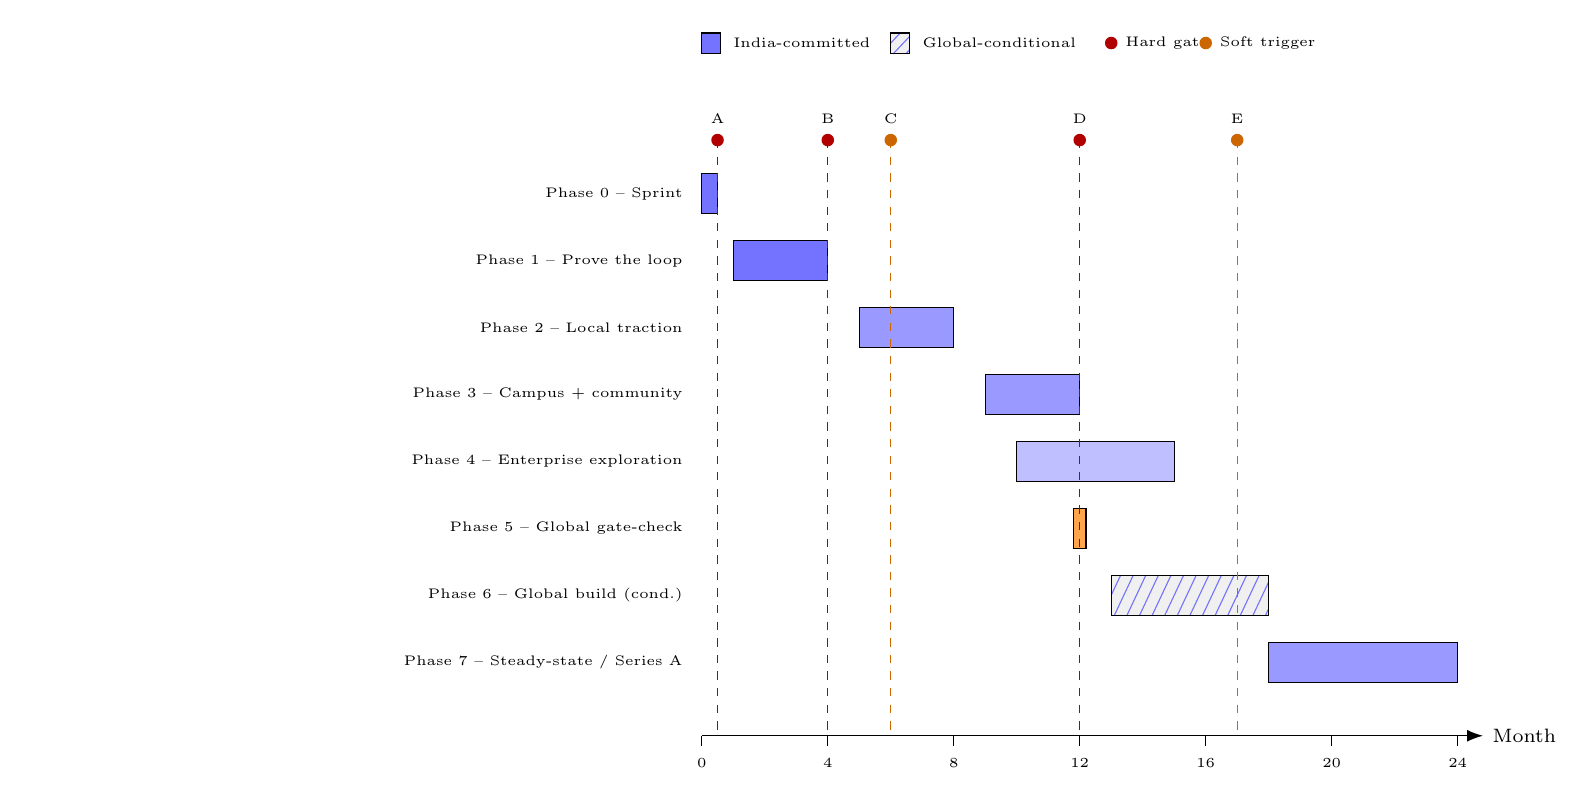
\begin{tikzpicture}[
  font=\scriptsize,
  x=0.40cm, y=0.85cm
]
% ---- Layout note ----
% Phase-name labels live in a fixed-width left margin (x = -8.6 to -0.2),
% right-aligned against x=0, so the timeline itself runs cleanly from
% month 0 to month 24 with no risk of labels overflowing the page on the right.
% Row y-coordinates (top = highest y)
\def\yZero{7.5}
\def\yOne{6.5}
\def\yTwo{5.5}
\def\yThree{4.5}
\def\yFour{3.5}
\def\yFive{2.5}
\def\ySix{1.5}
\def\ySeven{0.5}

% ---- Phase name labels (left margin, right-aligned) ----
\node[anchor=east, font=\tiny, text width=8.2cm, align=right] at (-0.3,\yZero) {Phase 0 -- Sprint};
\node[anchor=east, font=\tiny, text width=8.2cm, align=right] at (-0.3,\yOne) {Phase 1 -- Prove the loop};
\node[anchor=east, font=\tiny, text width=8.2cm, align=right] at (-0.3,\yTwo) {Phase 2 -- Local traction};
\node[anchor=east, font=\tiny, text width=8.2cm, align=right] at (-0.3,\yThree) {Phase 3 -- Campus + community};
\node[anchor=east, font=\tiny, text width=8.2cm, align=right] at (-0.3,\yFour) {Phase 4 -- Enterprise exploration};
\node[anchor=east, font=\tiny, text width=8.2cm, align=right] at (-0.3,\yFive) {Phase 5 -- Global gate-check};
\node[anchor=east, font=\tiny, text width=8.2cm, align=right] at (-0.3,\ySix) {Phase 6 -- Global build (cond.)};
\node[anchor=east, font=\tiny, text width=8.2cm, align=right] at (-0.3,\ySeven) {Phase 7 -- Steady-state / Series A};

% ---- Month axis (0..24), ticks every 4 months to keep node count low ----
\draw[-{Latex[length=2mm]}] (0,-0.6) -- (24.8,-0.6) node[right, font=\scriptsize] {Month};
\foreach \m in {0,4,8,12,16,20,24} {
  \draw (\m,-0.6) -- (\m,-0.75);
  \node[font=\tiny] at (\m,-1.0) {\m};
}

% ---- Phase bars ----
% Phase 0: Days 1-14 -- approximate as Month 0 to 0.5
\draw[fill=blue!55] (0,\yZero-0.3) rectangle (0.5,\yZero+0.3);

% Phase 1: Month 1-4
\draw[fill=blue!55] (1,\yOne-0.3) rectangle (4,\yOne+0.3);

% Phase 2: Month 5-8
\draw[fill=blue!40] (5,\yTwo-0.3) rectangle (8,\yTwo+0.3);

% Phase 3: Month 9-12
\draw[fill=blue!40] (9,\yThree-0.3) rectangle (12,\yThree+0.3);

% Phase 4: Month 10-15 (overlaps Phase 3)
\draw[fill=blue!25] (10,\yFour-0.3) rectangle (15,\yFour+0.3);

% Phase 5: Month 12 checkpoint (thin marker bar, not a duration)
\draw[fill=orange!70] (11.8,\yFive-0.3) rectangle (12.2,\yFive+0.3);

% Phase 6: Month 13-18, hatched (conditional Global) -- manual diagonal hatch, no extra TikZ library needed
\draw[fill=gray!12] (13,\ySix-0.3) rectangle (18,\ySix+0.3);
\begin{scope}
  \clip (13,\ySix-0.3) rectangle (18,\ySix+0.3);
  \foreach \k in {12.7,13.1,...,18.3} {
    \draw[blue!55, line width=0.4pt] (\k,\ySix-0.3) -- (\k+0.6,\ySix+0.3);
  }
\end{scope}
\draw (13,\ySix-0.3) rectangle (18,\ySix+0.3);

% Phase 7: Month 18-24 -- solid India portion (Global continuation implied, not separately hatched to keep node count low)
\draw[fill=blue!40] (18,\ySeven-0.3) rectangle (24,\ySeven+0.3);

% ---- Go/no-go gate markers (vertical dashed lines + circular gate markers, labeled A-E) ----
% Circles (a base TikZ shape) are used instead of the "diamond" shape so this figure
% compiles without the shapes.geometric library. Letters keyed to the gate list below.
\draw[dashed, red!70!black] (0.5,8.3) -- (0.5,-0.6);
\node[circle, fill=red!70!black, inner sep=1.6pt, label={[font=\tiny]above:A}] at (0.5,8.3) {};

\draw[dashed, red!70!black] (4,8.3) -- (4,-0.6);
\node[circle, fill=red!70!black, inner sep=1.6pt, label={[font=\tiny]above:B}] at (4,8.3) {};

\draw[dashed, orange!80!black] (6,8.3) -- (6,-0.6);
\node[circle, fill=orange!80!black, inner sep=1.6pt, label={[font=\tiny]above:C}] at (6,8.3) {};

\draw[dashed, red!70!black] (12,8.3) -- (12,-0.6);
\node[circle, fill=red!70!black, inner sep=1.6pt, label={[font=\tiny]above:D}] at (12,8.3) {};

\draw[dashed, orange!80!black] (17,8.3) -- (17,-0.6);
\node[circle, fill=orange!80!black, inner sep=1.6pt, label={[font=\tiny]above:E}] at (17,8.3) {};

% ---- Legend (compact, single row) ----
\draw[fill=blue!55] (0,9.6) rectangle (0.6,9.9);
\node[anchor=west, font=\tiny] at (0.7,9.75) {India-committed};
\draw[fill=gray!12] (6.0,9.6) rectangle (6.6,9.9);
\begin{scope}
  \clip (6.0,9.6) rectangle (6.6,9.9);
  \foreach \k in {5.7,6.1,...,6.9} {
    \draw[blue!55, line width=0.4pt] (\k,9.6) -- (\k+0.6,9.9);
  }
\end{scope}
\draw (6.0,9.6) rectangle (6.6,9.9);
\node[anchor=west, font=\tiny] at (6.7,9.75) {Global-conditional};
\node[circle, fill=red!70!black, inner sep=1.6pt] at (13.0,9.75) {};
\node[anchor=west, font=\tiny] at (13.15,9.75) {Hard gate};
\node[circle, fill=orange!80!black, inner sep=1.6pt] at (16.0,9.75) {};
\node[anchor=west, font=\tiny] at (16.15,9.75) {Soft trigger};

\end{tikzpicture}%
}
\caption{24-month Gantt-style roadmap with go/no-go gates. Bar shading: solid blue = India-committed work; hatched = Global Phase 2 work conditional on the Month-12 gate-check. Circular markers on the dashed vertical lines mark go/no-go gates -- red for hard stop/continue decisions, orange for softer triggers and checkpoints. Gate A: 1 verbal advertiser yes $\rightarrow$ go (Day 14). Gate B: MASTER-PLAN \S8.3 gate, Month 4 -- $\geq$2 advertisers paid and renewed, week-4 retention holds. Gate C: Tier-1 rate-card trigger, \textasciitilde Month 6 -- 5--10 advertisers signed. Gate D: Month 12 -- 10,000-user Tier-2 auction trigger and Global Phase 2 gate-check. Gate E: \textasciitilde Month 17 -- Global pilot fold-back check (must hit India's Phase-1 bar within 4 months or fold back). Full gate descriptions are given in Table~\ref{tab:roadmap} and Section~\ref{sec:roadmap-narrative}.}
\label{fig:roadmap-gantt}
\end{figure}

\section{Phase Narrative}
\label{sec:roadmap-narrative}

\textbf{Phase 0 (Days 1--14)} is the entire thesis compressed into two weeks: prove that one advertiser will say yes before writing more product code. \textbf{Phase 1 (Month 1--4)} is where the real go/no-go gate lives -- not a vanity-metrics checkpoint but a hard stop if advertisers do not renew or if developers churn once novelty fades. \textbf{Phases 2--4} (Month 5--15) layer on local scale, campus distribution, and an enterprise-adjacent motion, but every one of them is explicitly subordinate to the Phase-1 gate clearing first. \textbf{Phase 5} (Month 12) is deliberately drawn as a checkpoint, not a launch: Global Phase 2 is real optionality, not a commitment, and unlocks only if all three conditions in Table~\ref{tab:roadmap} hold simultaneously. \textbf{Phases 6--7} are the most speculative parts of this document and are included to show the team has thought about what success looks like at scale, not because they are funded or staffed today.

This roadmap should be read alongside the channel sequencing in Chapter~\ref{chap:gtm} (each phase activates new channels only as its predecessor's gate clears) and the risk register in Chapter~\ref{chap:risk-analysis} (notably R2's Tier-1 re-check on IdleAds rev-share pressure, which is explicitly re-triggered at the Phase 3 boundary above).

\chapter{Appendices}
\label{ch:appendices}

\section{Appendix A --- Glossary of Terms}
\label{app:glossary}

\begin{description}
  \item[Wait-state advertising] The category Devorix operates in: placing a
        sponsor message in the brief ``thinking'' / idle status moment of an AI
        coding tool, when the developer is waiting for the agent to respond.
        The defining feature is that the attention is captive and full ---
        unlike a sidebar the user scrolls past.

  \item[Status line / status-bar overlay] The thin text slot an AI coding tool
        renders during a thinking state (and the secondary VS~Code status-bar
        item). Devorix injects its sponsor line here via the configurable
        \texttt{statusLine} mechanism, \emph{non-patching} (see below).

  \item[Non-patching client] An integration that injects the sponsor line
        through a supported configuration hook and \emph{never} modifies the
        host tool's rendering layer, never reads code or prompts, and never
        touches the host tool's OAuth tokens. This is the basis of Devorix's
        platform-policy and ``we are not Kickbacks'' compliance posture.

  \item[Impression] A single billable display of a sponsor creative. A display
        counts as billable only when the creative has shown continuously for at
        least the billable impression length (5~seconds for v1) during an
        active session, and only after it passes server-side validity
        filtering.

  \item[Billable impression length] The minimum continuous display time before
        a display counts as a billable impression. Locked at \textbf{5~seconds}
        for the v1 build; 10~seconds retained as a documented, data-gated
        option.

  \item[Click] A counted event when a developer opens the optional click URL
        attached to a creative.

  \item[Fill rate] The percentage of available impression slots that are
        served a \emph{paid} (non-house) advertiser creative rather than a
        house ad. The single most sensitive variable in the financial model and
        a direct proxy for whether real advertiser demand exists; today
        $\sim$0\% (no advertisers).

  \item[House ad] A Devorix-controlled promotional creative served when no paid
        advertiser creative is available (e.g.\ at launch, before any
        advertiser exists). Generates a billable-shaped event at ₹0
        advertiser cost, used to validate the loop.

  \item[Tier 0 / Tier 1 / Tier 2] The three rungs of the locked hybrid pricing
        ladder. \textbf{Tier~0}: flat monthly sponsorships (₹10{,}000--
        15{,}000/mo) plus house ads, until $\sim$5 advertisers.
        \textbf{Tier~1}: a fixed-price CPM rate card (\$2--3 India / \$5--8
        Global), once 5--10 advertisers are signed. \textbf{Tier~2}: a
        real-time second-price auction, once 5{,}000+ DAU.

  \item[CPM] Cost per mille --- price per 1{,}000 impressions. The pricing
        basis for Tier~1 and above. The only independently audited real
        developer-advertising comp is Carbon Ads at \$1.60 CPM.

  \item[eCPM] Effective CPM --- revenue normalized to a per-1{,}000-impression
        figure, used to compare flat-fee Tier~0 deals against a CPM basis.

  \item[Block] A Tier~1 unit of inventory equal to 1{,}000 impressions; the
        unit an advertiser buys against the rate card.

  \item[DAU / WAU] Daily / Weekly Active Users --- developers with the client
        enabled and at least one session in the period. The 5{,}000+ \textbf{DAU}
        threshold triggers Tier~2.

  \item[Payout threshold] The accrued payable balance (locked at
        \textbf{₹300}) at which an automatic UPI payout is triggered.

  \item[Payable, not stored value] The regulatory framing of the developer's
        accrued balance: a debt Devorix owes, settled to a bank/UPI account on
        the threshold, with no load/spend/hold capability --- deliberately
        outside RBI's Prepaid Payment Instrument (PPI) definition.

  \item[UPI / VPA] Unified Payments Interface, India's real-time payment rail;
        a VPA (Virtual Payment Address, e.g.\ \texttt{name@bank}) is the
        UPI handle a payout is sent to.

  \item[RazorpayX] The payout provider; its Payouts API executes automated
        UPI/IMPS/NEFT/RTGS transfers with 24/7 instant UPI settlement.

  \item[Double-entry ledger] The money source of truth: every economic event
        posts as a balanced pair of entries, and a developer's visible balance
        is always a derived read (\,$\sum$ credits $-\,\sum$ debits\,), never a
        separately stored mutable field.

  \item[Raw / billable event separation] The architectural rule that raw
        impression events are stored separately from the fraud-filtered
        \texttt{billable\_events} that alone drive advertiser billing and
        developer payouts.

  \item[Atomic network] (Andrew Chen, \emph{The Cold Start Problem}) The
        smallest dense network that can stand on its own; Devorix's
        India-first, Ring-1-first plan is structurally an atomic-network
        strategy.

  \item[Three-ring niche] Devorix's advertiser targeting:
        \textbf{Ring~1} (AI-infra/dev-tool sellers to AI-building developers),
        \textbf{Ring~2} (India dev-economy sellers), \textbf{Ring~3} (global
        dev-tool brands, Phase~2 only).

  \item[Go/no-go gate] The locked month-4 test that governs continuation: at
        least two advertisers paid \emph{and} renewed, week-4 retention holds,
        and the founder still wants to run it.

  \item[Sweat equity] The founder's labour, modelled at ₹0 salary, so all
        margins are not fully loaded and exclude founder opportunity cost.
\end{description}

\section{Appendix B --- Locked Decisions (verbatim)}
\label{app:locked-decisions}

The table below reproduces \texttt{MASTER-PLAN.md} \S2 in full, with all
numbers verbatim. No decision in this table may be altered or hedged anywhere
in this document; they are stated as final facts.

{\small
\begin{longtable}{p{0.4cm} p{5.1cm} p{2.4cm} p{4.6cm}}
\caption{Locked decisions (\texttt{MASTER-PLAN.md} \S2, verbatim).}
\label{tab:locked-decisions} \\
\toprule
\textbf{\#} & \textbf{Decision} & \textbf{Status} & \textbf{Notes} \\
\midrule
\endfirsthead
\toprule
\textbf{\#} & \textbf{Decision} & \textbf{Status} & \textbf{Notes} \\
\midrule
\endhead
1 & Model = ads-to-devs (Kickbacks-style) & Decided & --- \\
\addlinespace
2 & First tool = Claude Code; client = non-patching/status-bar & Decided &
Enterprise-safe, avoids Kickbacks' ToS risk \\
\addlinespace
3 & Payout rail = RazorpayX UPI, accrue + batch & Decided & Re-verified
2026-06-28: RazorpayX Payouts API confirmed to support automated
UPI/IMPS/NEFT/RTGS, 24/7 instant settlement \\
\addlinespace
4 & Build = solo, founder-built MVP & Decided & --- \\
\addlinespace
5 & Public framing = ``sponsorship footer'' & Decided & From AI Studio
prototype \\
\addlinespace
6 & Adopt 3 Gemini prototype tools & Decided & Ad-Copy Generator (P1),
Wait-State Coach (P1), Workspace Analyzer (P2); core ad-serving/ledger must not
depend on Gemini \\
\addlinespace
7 & Entity/brand = ``Devorix'' / ``DEVORIX.'' & \textbf{DECIDED FINAL} & Renamed
from ``Async Returns'' / ``ASYNC.'' on 2026-06-28 per founder's explicit call.
Domain placeholder used across docs/code: devorix.ai --- not yet verified as
registered/available. \\
\addlinespace
8 & Budget/runway $\leq$ ₹1~lakh, low burn, solo & Founder constraint &
--- \\
\addlinespace
9 & Do NOT incorporate yet --- sole proprietor & Decided & Re-verified
2026-06-28, see \S7.1 \\
\addlinespace
10 & No GST registration yet (below ₹20L/yr threshold) & Decided &
Re-verified 2026-06-28, see \S7.1 \\
\addlinespace
11 & \textbf{Dev rev share = 50 / 50} & \textbf{DECIDED FINAL} & Closes the
50-vs-60-70\% open question. Overrides FINANCIAL\_MODEL's 40/60 and 01/03's
``60-70\% as install-war lever'' idea. \\
\addlinespace
12 & \textbf{Geographic sequencing: India first, Global = explicit Phase 2} &
\textbf{DECIDED FINAL} & Gated on the go/no-go criteria in \S8.3. PRD's
``non-India = non-goal'' is correct for now, not permanent. \\
\addlinespace
13 & \textbf{Payout threshold = ₹300} & \textbf{DECIDED FINAL} & Overrides
₹500 (05) and ₹250 (PRICING\_ARCHITECTURE) --- founder's call, splits
the difference \\
\addlinespace
14 & \textbf{Pricing model = hybrid ladder} --- Tier~0 (house ads +
opportunistic flat-fee deals, until $\sim$5 advertisers) $\rightarrow$ Tier~1
(real fixed-price CPM rate card, once 5--10 advertisers) $\rightarrow$ Tier~2
(real-time auction, once 5{,}000+ DAU) & \textbf{DECIDED FINAL} & Full detail
in \S5 \\
\addlinespace
15 & \textbf{Billable impression length = 5 seconds for v1 build}; 10 seconds
kept as a documented, data-gated option & \textbf{DECIDED FINAL for now} &
Founder asked to compare, not force a permanent choice --- see \S5.3 \\
\addlinespace
16 & \textbf{USD$\rightarrow$INR = ₹94} & \textbf{RE-VERIFIED 2026-06-28} &
Live mid-market $\sim$₹94.36--94.44. Replaces ₹86 (00), ₹83
(PRICING\_ARCHITECTURE, FINANCIAL\_MODEL); confirms ₹94.5 (05) was
right. \\
\addlinespace
17 & \textbf{Warm advertiser intros at sprint start = 0} (fully cold outreach) &
Founder constraint, newly confirmed & Adjusts sprint math, see \S6.3 \\
\addlinespace
18 & \textbf{Tier-1 rate-card CPM (once activated) = $\sim$\$2--3 India /
\$5--8 Global} & \textbf{DECIDED FINAL (planning number)} & Replaces \$8/\$15
(PRICING\_ARCHITECTURE) and \$5$\rightarrow$\$10-12 (FINANCIAL\_MODEL) ---
anchored to the one independently-audited real comp, not 4--10x it. Full
reasoning in \S5.4. Tagged \emph{Assumption} --- revisit with real fill
data. \\
\bottomrule
\end{longtable}
}

\section{Appendix C --- Methodology Note on Evidence Labelling}
\label{app:methodology}

Throughout this document, every non-trivial factual claim --- and especially
every number --- carries one of three labels, used consistently and never
blurred together through synthesis:

\begin{description}
  \item[Verified fact] Named, on-record, or independently multi-sourced. These
        are claims traceable to a primary source (e.g.\ a company's own
        disclosure, a regulator's documentation, or two or more independent
        reports). Example: ``India has 27~million developers on GitHub (2026)''
        --- attributed on record to GitHub's COO and corroborated across
        multiple outlets.

  \item[Industry estimate] Published by research firms or third parties,
        directionally consistent but without a single authoritative number, or
        self-reported. These are credible and useful as range/context but should
        not be treated as precise. Example: the AI code tools market at
        ``$\sim$\$9--9.5B (2026)'' across firms whose category boundaries
        disagree.

  \item[Internal assumption] Devorix's own model output, reasoning, or
        extrapolation --- not an externally researched fact. All figures past
        the locked, audited month-4 plan fall here. Example: the 12--24 month
        revenue scenarios, which are planner extrapolation, not workbook
        outputs.
\end{description}

Two conventions follow from this labelling. First, \textbf{the locked decisions
(Appendix~\ref{app:locked-decisions}) and the audited months-1--4 plan are the
only load-bearing inputs to the funding ask}; everything labelled Internal
assumption (the TAM ceiling, the 12--24 month curves, the agentic-economy
context) is optionality and direction, presented to explain \emph{why the bet
is worth taking if the near-term loop works}, never as something derived from
the financial workbooks. Second, where two source inputs disagreed, the
contradiction is \emph{resolved explicitly in the text} (e.g.\ the 18\%
workplace-usage vs.\ 28\%/24\% primary-tool-split adoption figures, reconciled
as measuring different populations) rather than silently dropped --- with the
more conservative, better-sourced figure adopted as the planning anchor and the
favourable figure carried forward only as a directional signal.

\section{Appendix D --- Note on the Multi-Agent Research Process}
\label{app:research-process}

In the interest of transparency about how this PRD was produced, this appendix
documents the research pipeline behind it.

The document was synthesized through a deliberate multi-agent workflow rather
than written in a single pass. The pipeline had three roles:

\begin{enumerate}
  \item \textbf{Explorer agents} performed broad, read-only fan-out research ---
        gathering named comparables, competitor launch mechanics, fund theses,
        regulatory specifics, and market figures from primary sources --- and
        returned findings with source attribution and confidence labels. Their
        job was to locate and verify evidence, not to draw conclusions.

  \item \textbf{Planner agents} structured that evidence into chapter-level
        synthesis: building the 24-month roadmap contingency tree, the moats
        verdict, the financial scenario extension, the persona set, and the
        risk register, while keeping the explorer's confidence labels intact and
        flagging open questions rather than papering over them.

  \item \textbf{An orchestrating synthesis pass} reconciled the planner outputs
        against the single source of truth (\texttt{MASTER-PLAN.md}), resolved
        every cross-document contradiction explicitly, enforced the locked
        decisions verbatim, and produced the final chapter text.
\end{enumerate}

The single source of truth throughout was \texttt{MASTER-PLAN.md}: where any
specialist input disagreed with it, the master plan won, and no locked decision
in Appendix~\ref{app:locked-decisions} was reopened at any stage. This process
is disclosed here so a reader can weigh the document's claims knowing how they
were assembled --- in particular, that the evidence labelling in
Appendix~\ref{app:methodology} was applied at the point of research collection
and preserved through synthesis, not retrofitted at the end.


% ---------------------------------------------------------------------------
\clearpage
\bibliographystyle{plainnat}
\bibliography{references}

\end{document}
